\chapter{The \textit{i}MGXS Spatial Homogenization Scheme}
\label{chap:unsupervised}

The preceding chapter illustrated the clustering of pin-wise \ac{MGXS} as a result of spatial self-shielding effects. It was shown that \ac{MGXS} clustering must be appropriately modeled to accurately resolve pin-wise U-238 capture rates. The \ac{LNS} spatial homogenization scheme was introduced to predict \ac{MGXS} clustering with a geometric template-like approach. The \ac{LNS} scheme was shown to achieve the same level of accuracy as degenerate homogenization while simultaneously accelerating the \ac{MC} tally convergence rate for simple benchmark problems. However, the \ac{LNS} scheme suffered from its inability to adapt to predict \ac{MGXS} clustering in geometries with water reflectors and steel baffles. In addition, the \ac{LNS} scheme did not scale well with the complexity of the core geometry, resulting in a large number of materials and thus an under-accelerated convergence rate. This chapter introduces an adaptable and scalable alternative to \ac{LNS} which uses unsupervised statistical learning methods to predict \ac{MGXS} clustering.

The novel homogenization methodology presented here -- referred to as \textit{inferential \ac{MGXS}} (\textit{i}\ac{MGXS}) spatial homogenization -- seeks to achieve the overarching goal of this thesis: to obtain Monte Carlo quality solutions with computationally efficient deterministic transport methods. The goal of \textit{i}\ac{MGXS} is to use algorithms developed by the machine learning community to infer \ac{MGXS} clusters directly from \ac{MC} tally data rather than predict clustering from an analysis of the core geometry. The \textit{i}\ac{MGXS} scheme is more generalizable and can flexibly accommodate arbitrary core heterogeneities better than \ac{LNS} or other geometric-based approaches which must be extensively customized for particular core geometries. In addition, the \textit{i}\ac{MGXS} scheme aims to greatly accelerate the convergence rate of \ac{MGXS} tallied with \ac{MC} with respect to the the degenerate and \ac{LNS} schemes as shown in Fig.~\ref{fig:chap10-flow-chart}.

\begin{figure}[h!]
\centering
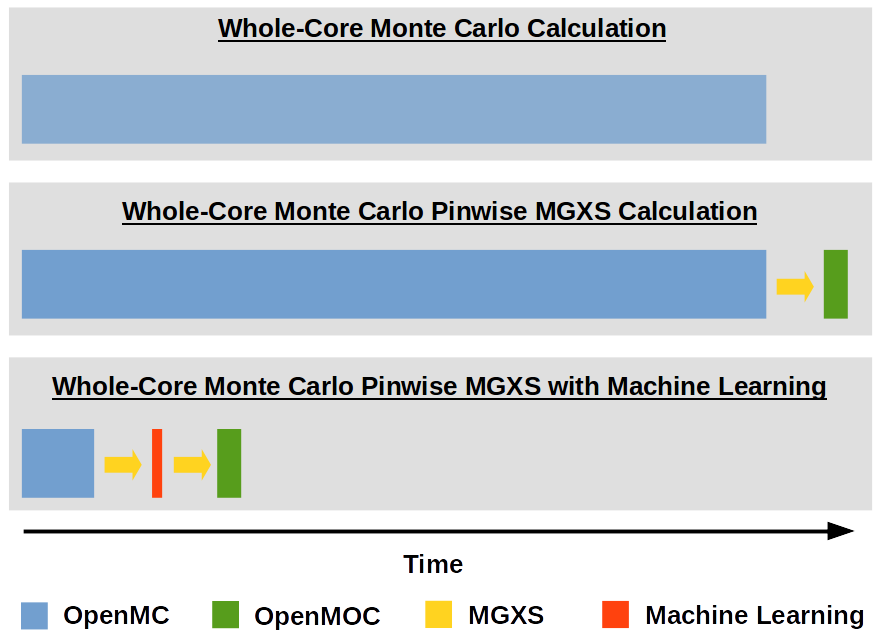
\includegraphics[width=0.6\linewidth]{figures/unsupervised/flow-chart}
\vspace{2mm}
\caption[Expected relative runtime for different homogenization schemes]{The expected relative runtime for the degenerate, \ac{LNS} and \textit{i}\ac{MGXS} spatial homogenization schemes with respect to a reference \ac{MC} calculation.}
\label{fig:chap10-flow-chart}
\end{figure}

This chapter begins by introducing a general latent variable model for \ac{MGXS} clustering which motivates \textit{i}\ac{MGXS} spatial homogenization in Sec.~\ref{sec:chap10-lsvm}. An overview of the \textit{i}\ac{MGXS} scheme is given in Sec.~\ref{sec:chap10-overview}, with in-depth presentations of the each stage of tally data pre-processing, including feature extraction (Sec.~\ref{sec:chap10-feature-extract}) and selection (Sec.~\ref{sec:chap10-feature-select}), and dimensionality reduction (Sec.~\ref{sec:chap10-dimension-reduce}). Sec.~\ref{subsec:chap10-train-predictor} highlights a few statistical clustering algorithms which may be interchangeably employed within the code framework for i\ac{MGXS} implemented for this thesis. A few heuristics for unsupervised cluster model selection are discussed in Sec.~\ref{sec:chap10-model-select}. Sec.~\ref{sec:chap10-imgxs-homogenization} discusses the track density-weighting used to spatially homogenize the pin-wise \ac{MGXS}. Finally, Sec.~\ref{sec:chap10-cluster-geometries} illustrates the material configurations produced by the \textit{i}\ac{MGXS} scheme for the heterogeneous \ac{PWR} benchmarks studied in this thesis. The eigenvalues and pin-wise fission and U-238 capture rates produced with the \textit{i}\ac{MGXS} scheme are evaluated in the following chapter.

%Finally, Sec.~\ref{sec:chap10-cluster} details two approaches used to evaluate the ideal and realized convergence rates of the \textit{i}\ac{MGXS} scheme. 



%%%%%%%%%%%%%%%%%%%%%%%%%%%%%%%%%%%%%%%%%%%%%%%%%%%%%%%%%%%%%%%%%%%%%%%%%%%%%%%%
\section{Latent Spectral Variable Model}
\label{sec:chap10-lsvm}

[REDACTED: to include or no??]

%
%This section postulates the existence of a probability distribution from which pin-wise \ac{MGXS} are drawn when generated from Monte Carlo tallies. In particular, this section introduces a \textit{latent variable model} -- termed the \ac{LSVM} -- which encapsulates the spatial self-shielding effects in heterogeneous geometries that leads to clustering of pin-wise \ac{MGXS}. \ac{LSVM} inspires the development of the unsupervised statistical clustering methodology for spatial homogenization that is the topic of this and the following chapter. Latent variable models are a widely used theoretical construct for representing \textit{hidden variables} which parameterize the probability distributions that are thought to have produced some observed dataset. This section loosely follows Bishop's presentation of probabilistic mixture models~\cite{bishop2006pattern}, including the mathematical notation frequently employed by discussions of latent variable models in the statistics and machine learning literature. Sec.~\ref{subsec:chap10-lsvm-math} introduces the concept of latent spectral variables which dictate a parametrization of a mixture distribution which generated the pin-wise \ac{MGXS}. Sec.~\ref{subsec:chap10-lsvm-graph} illustrates \ac{LSVM} with a few graphical models.
%
%%Sec.~\ref{subsec:chap10-lsvm-additive-noise} begins by decompose \ac{MC} estimates for \ac{MGXS} into a multi-component additive noise model. 
%
%%%%%%%%%%%%%%%%%%%%%%%%%%%%%%%%%%%
%\subsection{Latent Spectral Variables}
%\label{subsec:chap10-lsvm-math}
%
%
%
%As shown in Chap.~\ref{chap:spatial}, spatial self-shielding effects from geometric heteoregneities leads to clustering of pin-wise \ac{MGXS}. This may 
%
%The \ac{MGXS} clustering effects induced by spatial self-shielding from various core heterogeneities, 
%
%\begin{align}
%\label{eqn:chap10-mgxs-offsets}
%\sigma_{k} &= \pi_{k,1}\Delta_{1} + \pi_{k,2}\Delta_{2} + \cdots + \pi_{k,M}\Delta_{M} \\
%&= \displaystyle\sum\limits_{m=1}^{M}\pi_{k,m}\Delta_{m}
%\end{align}
%
%
%
%As discussed in Sec.~\ref{sec:chap3-mgxs-gen}, the \ac{MGXS} tallied by \ac{MC} are random variables each with an estimated sample mean and variance. \ac{LSVM} describes the probability distribution that produced the population of \ac{MGXS} random variables for a particular type of material zone. In this thesis, \ac{LSVM} is used to describe the population of pin-wise microscopic \ac{MGXS} for all instances of fuel pins of a particular enrichment in a core geometry. For example, the tallied pin-wise microscopic \ac{MGXS} $\hat{\sigma}_{x,i,k,g}$ for some reaction $x$, nuclide $i$, fuel pin instance $k$ and energy group $g$ constitute the dataset produced by some probability distribution. \ac{LSVM} hypothesizes that the statistical process which generated the \ac{MGXS} dataset is a \textit{mixture model distribution} with $M$ mixture components. Each component $m$ is a normalized distribution $p(\hat{\sigma}_{x,i,k,g}; \boldsymbol{\theta}_{m})$ parameterized by vector $\boldsymbol{\theta}_{m}$, where for simplicity is assumed that all components are from the same parametric family of distributions\footnote{This restriction may not accurately characterize the mixtures components which generates pin-wise \ac{MGXS}, but is useful to simplify the number of symbols needed to introduces \ac{LSVM}.}\textsuperscript{,}\footnote{If the components are normal then $p(\hat{\sigma}_{x,i,k,g}; \boldsymbol{\theta}_{m}) = \mathcal{N}(\boldsymbol{\theta}_{m})$ with parameter vector $\boldsymbol{\theta}_{m} = \left[\mu_{m} \;\; \sigma_{m}\right]^{T}$.}. The components are combined in a linear superposition with \textit{mixing coefficients} $\pi_{m}$ to produce the mixture model distribution $f(\hat{\sigma}_{x,i,k,g})$:
%
%\begin{equation}
%\label{eqn:chap10-mix-model}
%f(\hat{\sigma}_{x,i,k,g}) = \displaystyle\sum\limits_{m=1}^{M} \pi_{m} p(\Delta_{m}; \boldsymbol{\theta}_{m})
%\end{equation}
%
%%\begin{equation}
%%\label{eqn:chap10-mix-model}
%%f(\hat{\sigma}_{x,i,k,g}) = \displaystyle\sum\limits_{m=1}^{M} \pi_{m} p(\hat{\sigma}_{x,i,k,g}; \boldsymbol{\theta}_{m})
%%\end{equation}
%
%\noindent where the coefficients ${\pi_{m}}$ are defined to sum to unity such that the model is normalized:
%
%%If each mixture has $N$ parameters (\textit{e.g}, $|\boldsymbol{\theta}| = N$), then $\boldsymbol{\Theta}$ is the $K \times N$ matrix of mixture model parameters, and $\boldsymbol{\Lambda}$ is the $K$-dimensional vector $\boldsymbol{\lambda} = \left[\lambda_{1} \;\; \lambda_{2} \;\; \dots \;\; \lambda_{m}\right]^{T}$ of mixing weights. The weights are defined to sum to unity such that the mixture model is normalized:
%
%\begin{equation}
%\label{eqn:chap10-mix-weights-norm}
%0 \le \pi_{m} \le 1 \;\;\; , \;\;\; \displaystyle\sum\limits_{m=1}^{M} \pi_{m} = 1
%\end{equation}
%
%The statistical model in Eqn.~\ref{eqn:chap10-mix-model} is a complete prescription for how the dataset of $\hat{\sigma}_{x,i,k,g}$ are generated for the population of fuel pins. In particular, \ac{LSVM} hypothesizes the existence of a \textit{latent spectral variable} $z_{k}$ for each fuel pin instance. Furthermore, \ac{LSVM} posits that the latent spectral variable may assume $Z$ integral values such that $z_{k} \in \{1, 2, \dots, Z\}$. From a practical standpoint, the latent spectral variable corresonds to the shape of the flux across energy group $g$ in fuel pin instance $k$\footnote{The shape of the flux across energy group $g$ cannot be directly observed from energy-integrated \ac{MC} tally data, and hence the spectral variable is a latent or hidden variable.}. \ac{LSVM} prescribes a one-to-one mapping from each possible value of the latent variable $z_{k}$ to a corresponding vector of mixing coefficients $\boldsymbol{\pi}(z_{k})$:
%
%\begin{equation}
%\label{eqn:chap10-mix-coeffs}
%\boldsymbol{\pi}(z_{k}) = \boldsymbol{\pi}_{k} = \left[\lambda_{1,k} \;\; \lambda_{2,k} \;\; \cdots \;\; \lambda_{m,k}\right]^{T}
%\end{equation}
%
%\noindent used to generate the dataset of $\hat{\sigma}_{x,i,k,g}$ according to the following stochastic process:
%
%\begin{equation}
%\label{eqn:chap10-lsvm}
%\hat{\sigma}_{x,i,k,g} \;\; \sim \;\; f(\hat{\sigma}_{x,i,k,g})
%\end{equation}
%
%%\ell \;\; &\sim \;\; \text{Multinomial}(p_{1}, p_{2}, \dots, p_{M}) \\
%% \boldsymbol{\lambda} \;\; &\sim \;\; \text{Categorical}(p_{1}, p_{2}, \dots, p_{M}) \\
%
%%\footnote{The symbol $\phi$ is adopted from the widely used notation for latent variables in the machine learning literature and should not be confused for the neutron flux.}
%
%
%%%%%%%%%%%%%%%%%%%%%%%%%%%%%%%%%%%%%%%%%%%%
%\subsection{An Additive Noise Model for MGXS}
%\label{subsec:chap10-lsvm-additive-noise}
%
%Additive noise models are useful theoretical construct widely considered in information theory to model many stochastic processes found in nature. This section introduces an additive noise model for \ac{MC} estimates for \ac{MGXS}. Consider an arbitrary propbability distribution $f_{x,i,k,g}(\cdot)$ from which the estimated pin-wise \ac{MGXS} $\hat{\sigma}_{x,i,k,g}$ (Eqn.~\ref{eqn:chap3-general-micro}) for reaction $x$, nuclide $i$, spatial zone $k$ and energy group $g$ are drawn:
%
%\begin{equation}
%\label{eqn:chap10-mgxs-draw}
%\hat{\sigma}_{x,i,k,g} \;\; \sim \;\; f_{x,i,k,g}(\hat{\sigma})
%\end{equation}
%
%\noindent The reaction $x$, nuclide $i$ and energy group $g$ subscripts may dropped for brevity:
%
%\begin{equation}
%\label{eqn:chap10-mgxs-draw-brevity}
%\hat{\sigma}_{k} \;\; \sim \;\; f_{k}(\hat{\sigma})
%\end{equation}
%
%An additive noise model may treat the \ac{MC} estimate for the \ac{MGXS} $\hat{\sigma}_{k}$ as the composition of the ``true'' \ac{MGXS} $\sigma_{k}$ (\textit{i.e.}, the expectation of $f(\hat{\sigma}_{k})$, or $\mathbb{E}[\hat{\sigma}_{k}]$) and a random ``noise'' term $\epsilon_{k}$. The noise $\epsilon_{k}$ is a random variable drawn from an arbitrary distribution $p(\epsilon; \boldsymbol{\theta}_{k})$ parameterized by $\boldsymbol{\theta}_{k}$ which represents the statistical uncertainty of the \ac{MC} estimate\footnote{If the \ac{MC} realizations are i.i.d. then the noise variables are normally distributed.}. The additive noise model for $\hat{\sigma}_{k}$ is then simply the sum of the true \ac{MGXS} and the random noise terms:
%
%\begin{align}
%\label{eqn:chap10-add-noise}
%\epsilon_{k} \;\; &\sim \;\; p(\epsilon; \boldsymbol{\theta}_{k}) \\
%\hat{\sigma}_{k} &= \sigma_{k} + \epsilon_{k}
%\end{align}
%
%As shown in Chap.~\ref{}, spatial self-shielding effects from geometric heteoregneities leads to clustering of pin-wise \ac{MGXS}. This may 
%
%The \ac{MGXS} clustering effects induced by spatial self-shielding from various core heterogeneities, 
%
%\begin{align}
%\label{eqn:chap10-mgxs-offsets}
%\sigma_{k} &= \pi_{k,1}\Delta_{1} + \pi_{k,2}\Delta_{2} + \cdots + \pi_{k,M}\Delta_{M} \\
%&= \displaystyle\sum\limits_{m=1}^{M}\pi_{k,m}\Delta_{m}
%\end{align}
%
%
%\begin{align}
%\label{eqn:chap10-mgxs-noise}
%\epsilon_{m} \;\; &\sim \;\; p(\epsilon; \boldsymbol{\theta}_{m}) \\
%\hat{\Delta}_{m} &= \Delta_{m} + \epsilon_{m}
%\end{align}
%
%compose the noise into different spectral effects
%
%\begin{align}
%\label{eqn:chap10-sum-noise}
%\hat{\sigma}_{k} &= \pi_{k,1}\hat{\Delta}_{1} + \pi_{k,2}\hat{\Delta}_{2} + \cdots + \pi_{k,M}\hat{\Delta}_{M} \\
%&= \pi_{k,1}\left(\Delta_{1} + \epsilon_{1}\right) + \pi_{k,2}\left(\Delta_{2} + \epsilon_{m}\right) + \cdots + \pi_{k,M}\left(\Delta_{M} + \epsilon_{m}\right) \\
%&= \displaystyle\sum\limits_{m=1}^{M}\pi_{k,m}\left(\Delta_{m} + \epsilon_{m}\right) \\
%&= \displaystyle\sum\limits_{m=1}^{M}\pi_{k,m}\Delta_{m} + \displaystyle\sum\limits_{m=1}^{M}\pi_{k,m}\epsilon_{m} \\
%% &= \sigma_{k} + \displaystyle\sum\limits_{m=1}^{M}\pi_{k,m}\epsilon_{m}
%\end{align}
%
%
%%%%%%%%%%%%%%%%%%%%%%%%%%%%%
%\subsection{Graphical Plate Notation}
%\label{subsec:chap10-lsvm-graph}
%
%\begin{figure}
%\centering
%\begin{tikzpicture}
%\tikzstyle{main}=[circle, minimum size = 8mm, thick, draw =black!80, node distance = 16mm]
%\tikzstyle{param}=[regular polygon, regular polygon sides=4, minimum size = 8mm, thick, draw =black!80, node distance = 16mm]
%  \node[param] (zk) [label=above:$z_k$] { };
%  \node[param] (theta) [left=of zk,label=left:$\boldsymbol{\Theta}$] { };
%  \node[main, fill = black!20] (sigma) [below=of zk, label=below:$\hat{\sigma}_{x,i,k,g}$] { };
%  \node[param] (pi) [left=of sigma,label=left:$\boldsymbol{\pi}$] { };
%   \draw[dagconn] (zk) to (sigma);
%   \draw[dagconn] (theta) to (sigma);
%   \draw[dagconn] (pi) to (sigma);
%   \node[plate=K, inner sep=20pt, fit=(zk) (sigma)] (plate1) {};
%\end{tikzpicture}
%\vspace{4mm}
%\caption[Graphical model for LSVM for a specific reactor configuration]{A graphical model to describe \ac{LSVM} for a specific reactor configuration.}
%\label{fig:chap10-lsvm-plate}
%\end{figure}
%
%\begin{figure}
%\centering
%\begin{tikzpicture}
%\tikzstyle{main}=[circle, minimum size = 8mm, thick, draw =black!80, node distance = 16mm]
%\tikzstyle{param}=[regular polygon, regular polygon sides=4, minimum size = 8mm, thick, draw =black!80, node distance = 16mm]
%  \node[param] (alpha) [label=above:$\boldsymbol{\alpha}$] { };
%  \node[main] (theta) [below left=of alpha,label=above:$\theta_{m}$] { };
%  \node[main] (pi) [below right=of alpha,label=above:$\pi_{m}$] { };
%  \node[param] (zk) [below=of theta,label=below:$z_k$] { };
%  \node[main, fill = black!20] (sigma) [below=of pi, label=below:$\hat{\sigma}_{x,i,k,g}$] { };
%   \draw[dagconn] (alpha) to (theta);
%   \draw[dagconn] (alpha) to (pi);
%   \draw[dagconn] (zk) to (sigma);
%   \draw[dagconn] (theta) to (sigma);
%   \draw[dagconn] (pi) to (sigma);
%   \node[plate=M, inner sep=20pt, fit=(theta) (pi)] (plate1) {};
%   \node[plate=K, inner sep=20pt, fit=(zk) (sigma)] (plate2) {};
%\end{tikzpicture}
%\vspace{4mm}
%\caption[Graphical model for LSVM for an arbitrary reactor configuration]{A graphical model to describe \ac{LSVM} for an arbitrary reactor configuration.}
%\label{fig:chap10-lsvm-plate-general}
%\end{figure}
%
%
%-we need to infer the latent variables $z_{k}$ for each fuel pin instance!!!
%-mention covariance between samples - the could be correlated
%-three goals:
%  -infer number of points/pins in each set
%  -infer conditional probabilities?
%  -assign each region to the most likely set?
%-is this section needed???
%-mention possibility of a multi-level latent variable model
%-mention bayesian approach to solving this using maximum likelihood


%%%%%%%%%%%%%%%%%%%%%%%%%%%%%%%%%%%%%%%%%%%%%%%%%%%%%%%%%%%%%%%%%%%%%%%%%%%%%%%
\section{Overview of \textit{i}MGXS}
\label{sec:chap10-overview}

The \textit{i}\ac{MGXS} spatial homogenization scheme is a multi-stage data processing \textit{pipeline}. The objective of the scheme is to infer the optimal assignment of cluster labels to fuel pin instances directly from \ac{MC} tally data. The cluster labels output by \textit{i}\ac{MGXS} are then used to generate track density-weighted \ac{MGXS} (see Sec.~\ref{subsec:chap9-lns-math}) for each cluster of fuel pin instances using the same process as that employed by \ac{LNS} homogenization (Eqn.~\ref{eqn:chap9-lns-micro}). The \textit{i}\ac{MGXS} methodology differs from the \ac{LNS} scheme in that it makes no consideration of the geometry and materials configuration and only examines tallied \ac{MC} tally data when assigning cluster labels to fuel pin instances.

A high-level overview of the various stages of the \textit{i}\ac{MGXS} data processing pipeline is illustrated in Fig.~\ref{fig:chap10-pipeline}. The \textit{i}\ac{MGXS} pipeline may be configured in various ways and this thesis makes no presumption that the incarnation presented in Fig.~\ref{fig:chap10-pipeline} is the best or most reliable version. Future work may develop schemes which improve upon the particular formulation of \textit{i}\ac{MGXS} presented in this thesis. Irregardless of the particular configuration, the overarching concept is that the \textit{i}\ac{MGXS} pipeline provides a \textit{mapping} between \ac{MC} tally data and cluster labels for each fuel pin\footnote{Similarly, the \ac{LNS} scheme defines a mapping between the combinatorial geometry and the cluster labels.}. Each of the six stages in Fig.~\ref{fig:chap10-pipeline} is detailed in the following sections of this thesis.

\begin{figure}[h!]
\centering
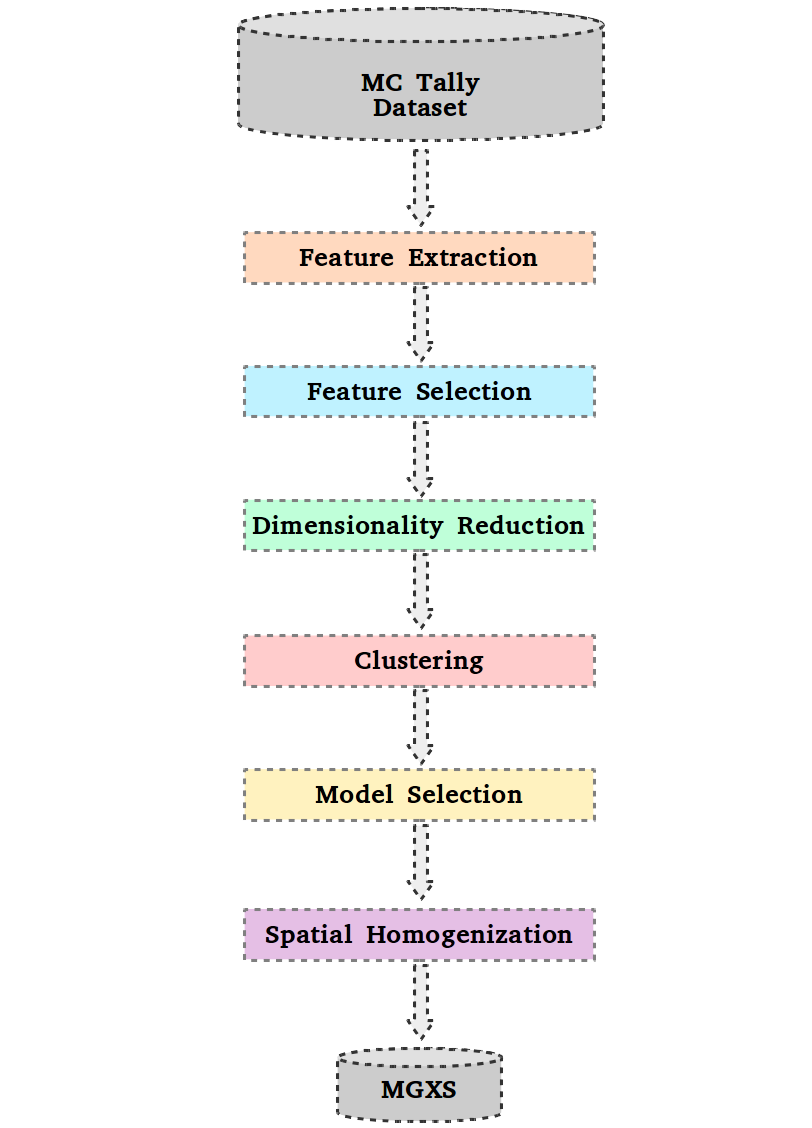
\includegraphics[width=0.655\linewidth]{figures/unsupervised/pipeline}
\vspace{2mm}
\caption[MGXS pipeline]{The multi-stage \textit{i}\ac{MGXS} data processing pipeline.}
\label{fig:chap10-pipeline}
\end{figure}


%%%%%%%%%%%%%%%%%%%%%%%%%%%%%%%%%%%%%%%%%%%%%%%%%%%%%%%%%%%%%%%%%%%%%%%%%%%%%%%
\section{Feature Extraction}
\label{sec:chap10-feature-extract}

The \textit{feature extraction} stage in the data processing pipeline in Fig.~\ref{fig:chap10-pipeline} builds \textit{features} from \ac{MC} tally data. In machine learning, features are simply variables which are used as inputs to a predictive model. Features may be engineered based upon prior domain knowledge or inferred from automated feature learning algorithms such as neural networks. In the context of \textit{i}\ac{MGXS}, features are restricted to tallies, or combinations of tallies, from \ac{MC} simulations which provide information about which fuel pin instances experience similar spatial self-shielding effects. For example, the pin-wise \ac{MGXS} $\hat{\sigma}_{x,i,k,g}$ themselves may be used as features since they exhibit the very clustering effect which \textit{i}\ac{MGXS} attempts to predict\footnote{Using the pin-wise \ac{MGXS} as the only feature(s) for unsupervised clustering would be equivalent to specifying boundaries between the samples illustrated in the rug plots in Sec.~\ref{subsec:chap9-histograms}.}. Other tallied quantities may also be used as features for predicting which fuel pin instances have similarly self-shielded \ac{MGXS}. The goal of extracting \textit{i}\ac{MGXS} features is to enable machine learning algorithms to identify \ac{MGXS} clusters as quickly as possible from ``noisy'' or unconverged tally data.

The \textit{i}\ac{MGXS} scheme splits the \ac{MC} tally dataset up into \textit{samples} for each particular instance $k$ of a fuel pin as illustrated in Fig.~\ref{fig:chap10-feature-extract}. A \textit{sample} is a random vector with $J$ entries for each feature $\hat{f}_{j,k}$ corresponding to a particular instance $k$ of a fuel pin. A sample may be comprised of features derived from \ac{MC} tally data for one or multiple nuclides, energy groups and/or reaction types. Ideally, the features should maximize the \textit{separation distance} in feature space $\{f_{1}, f_{2}, \dots, f_{J}\}$ between samples from the same cluster. Since features in \textit{i}\ac{MGXS} are tallied quantities from \ac{MC} simulations, some samples may include ``outlier'' feature realizations which take on values far removed from the ``true'' value of the feature\footnote{The ``true'' values are the expected values for each feature.}. Outliers may result in the incorrect assignment of cluster labels to fuel pin instances. The predictive models used in \textit{i}\ac{MGXS} are trained with the complete vector of features in order to mitigate the sensitivity of the models to outlier features and minimize the frequency of mis-labeled cluster assignments.

\begin{figure}[h!]
\centering
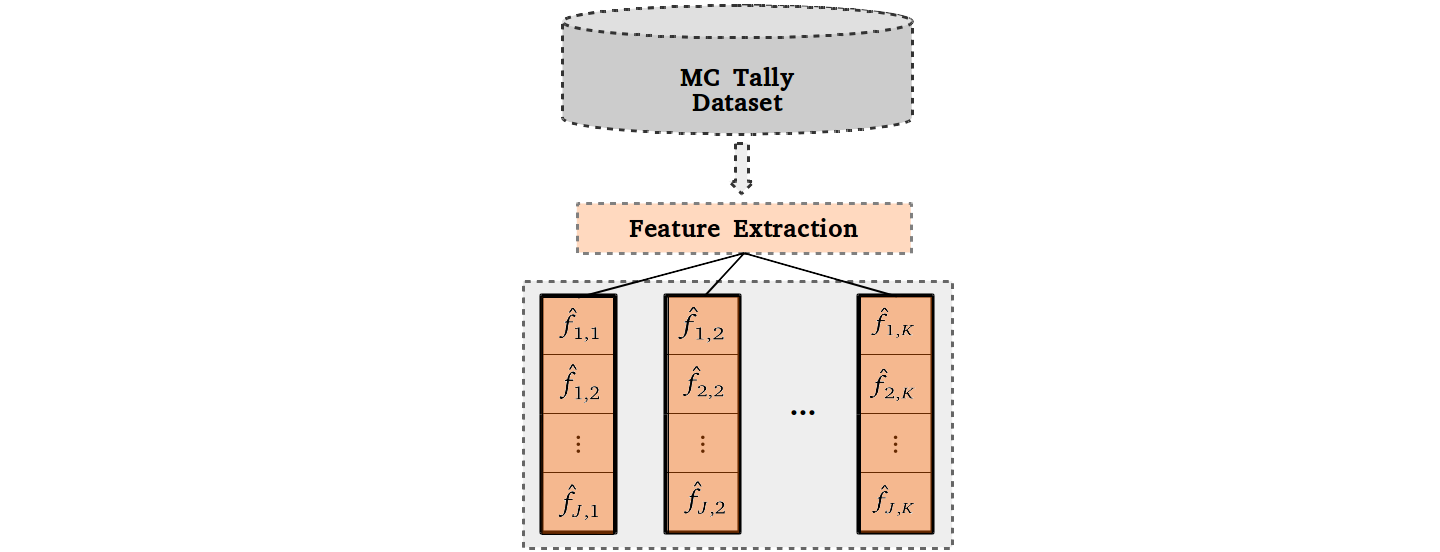
\includegraphics[width=0.9\linewidth]{figures/unsupervised/features/engineering/extract}
\vspace{2mm}
\caption[\textit{i}MGXS sample feature extraction]{\textit{i}\ac{MGXS} extracts feature vectors for each sample (fuel pin instance).}
\label{fig:chap10-feature-extract}
\end{figure}

In addition, it should be noted that features may not necessarily be defined for the same energy group structure as the \ac{MGXS} one wishes to cluster. For example, some or all features may be tallied on a relatively coarse energy group structure in order to minimize their \ac{MC} statistical uncertainties. It is in fact be beneficial to tally features in few groups in order to identify clusters with fewer \ac{MC} particle histories than would needed to distinguish structure from ``noisy'' fine group features.
These coarse group features may be input to a clustering algorithm for spatial homogenization of pin-wise \ac{MGXS} defined on a fine(r) energy group structure. For example, the following sections and chapters cluster features defined for a coarse 2-group structure in order to assign each fuel pin to a cluster for spatial homogenization of the ``fine'' 70-group pin-wise \ac{MGXS} data needed to minimize reaction rate errors to 1 -- 2\% or less.

The following sections introduce the features employed by \textit{i}\ac{MGXS} in this and the following chapter. These include the pin-wise \ac{MGXS} and their statistical uncertainties (Sec.~\ref{subsec:chap10-stat-uncertainty}), as well as features referred to as fractional reactivites (Sec.~\ref{subsec:chap10-frac-reactivity}), spectral indices (Sec.~\ref{subsec:chap10-spec-index}) and nuclide fractions (Sec.~\ref{subsec:chap10-nuclide-frac}). Each feature is specific to a fuel pin instance, and may further be distinguished for one or more nuclides, energy groups and/or reaction types. Each feature is presented with accompanying illustrations generated using a custom-built tool to visualize \textit{i}\ac{MGXS} features~\cite{abel2016bokeh}, and which correspond to the 1.6\% enriched fuel assembly benchmark.

%The clustering algoritms used in \textit{i}\ac{MGXS} may more easily identify clusters from the less ``noisy'' feature data, and the cluster labels used to spatially homogenize fine(r) group pin-wise \ac{MGXS}. 

%first paragraph: motivationa 
%  -could cluster multiple microscopic \ac{MGXS} simultaneously - nuclides, reactions, groups

%%%%%%%%%%%%%%%%%%%%%%%%%%%%%%%%%%%%%%%%%
\subsection{MGXS Statistical Uncertainty}
\label{subsec:chap10-stat-uncertainty}

The statistical uncertainty for each pin-wise \ac{MGXS} may be a useful feature to indicate clustering effects. In particular, the standard deviation of the sample mean is easily obtained from OpenMC tallies and can be incldued in the feature vector for each fuel pin instance. The intuition behind this is that the track densities -- and therefore, the statistical uncertainties -- in different fuel pins may reflect the spatial self-shielding effects experienced by different types of fuel pins. For example, the thermal flux track density will vary for fuel pins with differential moderation from \acp{CRGT}, reflectors, etc., which may present itself through a systematic clustering of the statistical uncertainties. Similarly, the track density will vary for fuel pins which experience varying degrees of spatial self-shielding in U-238 resonance groups -- which greatly impacts the resultant \ac{MGXS} in those groups -- and may be identifiable in the \ac{MGXS} uncertainties.

The statistical uncertainty feature is illustrated with scatter plots in Figs.~\ref{fig:chap10-fiss-mean-std} and~\ref{fig:chap10-capt-mean-std} for 2-group U-235 fission and U-238 capture \ac{MGXS} data, respectively. The scatter plots include a single data point for each of the 264 fuel pins in the 1.6\% enriched fuel assembly benchmark. The $x$ and $y$ coordinates correspond to the tallied \ac{MGXS} means $\hat{\sigma}_{x,i,k,g}$ and standard deviations $\sigma_{\hat{\sigma}_{x,i,k,g}}$ in units of barns, respectively. The complete datasets are illustrated in Figs.~\ref{fig:chap10-fiss-mean-std-mgxs} and~\ref{fig:chap10-capt-mean-std-mgxs}. The interactive \textit{i}\ac{MGXS} visualization tool was used to select clusters of \ac{MGXS} and plot the geometry to indicate the associated fuel pins, as displayed in Figs.~\Crefrange{fig:chap10-fiss-mean-std-geom-2}{fig:chap10-fiss-mean-std-mgxs-3} and~\Crefrange{fig:chap10-capt-mean-std-geom-2}{fig:chap10-capt-mean-std-mgxs-3} for the fission and capture \ac{MGXS}, respectively. The figures illustrate that the U-235 \ac{MGXS} uncertainties are smallest for the fuel pins with the most differential moderation (\textit{i.e.}, pin facially adjacent to \acp{CRGT}) and a relatively larger thermal flux track density. In contrast, the U-238 capture \ac{MGXS} uncertainties are largest for those pins with the most differential moderation due to the smaller fast-to-thermal flux ratio in these pins.

Notwithstanding the motivation to use the statistical uncertainties, there are also potential challenges associated with this approach. First, it would be possible for two different fuel pin instances to experience the same flux shape -- and therefore have the same \ac{MGXS} -- but very different flux magnitudes. Although the \ac{MGXS} uncertainties for the two pins would be very different, this would not accurately reflect the fact that the two pins should ideally be assigned to the same \ac{MGXS} cluster. Furthermore, error propagation theory only approximates the \ac{MGXS} uncertainties since it neglects the covariance between reaction rate and flux tallies. This approximation overestimates the \ac{MGXS} uncertainties since the reaction rate and flux tallies are highly correlated. As a result, the uncertainties may not exhibit systematic trends with poorly converged \ac{MC} data since the uncertainties will be larger than their ``true'' values. However, these are not reasons to eliminate the uncertainties as a possible feature; rather, it incites the need for robust feature selection as discussed in Sec.~\ref{sec:chap10-feature-select}.

%\begin{equation}
%\label{eqn:chap10-rel-err}
%\eta_{x,i,k,g} = \frac{\sigma_{\hat{\sigma}_{x,i,k,g}}}{\hat{\sigma}_{x,i,k,g}}
%\end{equation}

\begin{figure}[h!]
\centering
\begin{subfigure}{0.45\textwidth}
  \centering
  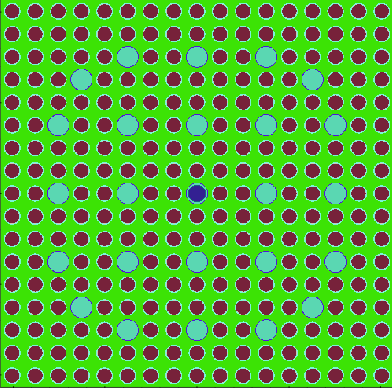
\includegraphics[width=0.9\linewidth]{figures/unsupervised/features/assm-16/geometry}
  \caption{}
  \label{fig:chap10-fiss-mean-std-geom}
\end{subfigure}%
\begin{subfigure}{0.45\textwidth}
  \centering
  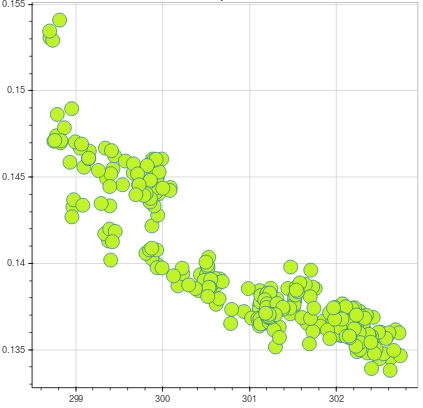
\includegraphics[width=0.9\linewidth]{figures/unsupervised/features/assm-16/u235-fiss/mean-std/mgxs}
  \caption{}
  \label{fig:chap10-fiss-mean-std-mgxs}
\end{subfigure}
\begin{subfigure}{0.45\textwidth}
  \centering
  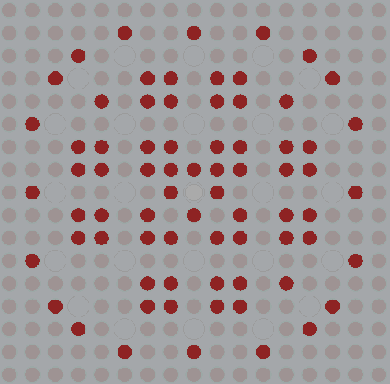
\includegraphics[width=0.9\linewidth]{figures/unsupervised/features/assm-16/u235-fiss/mean-std/geometry-2}
  \caption{}
  \label{fig:chap10-fiss-mean-std-geom-2}
\end{subfigure}%
\begin{subfigure}{0.45\textwidth}
  \centering
  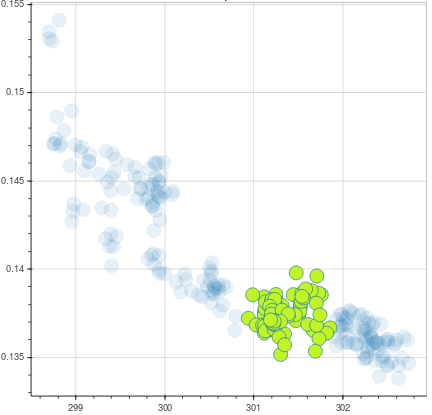
\includegraphics[width=0.9\linewidth]{figures/unsupervised/features/assm-16/u235-fiss/mean-std/mgxs-2}
  \caption{}
  \label{fig:chap10-fiss-mean-std-mgxs-2}
\end{subfigure}
\begin{subfigure}{0.45\textwidth}
  \centering
  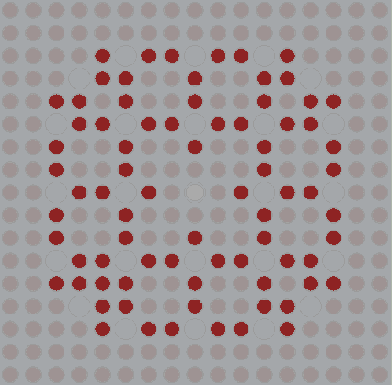
\includegraphics[width=0.9\linewidth]{figures/unsupervised/features/assm-16/u235-fiss/mean-std/geometry-3}
  \caption{}
  \label{fig:chap10-fiss-mean-std-geom-3}
\end{subfigure}%
\begin{subfigure}{0.45\textwidth}
  \centering
  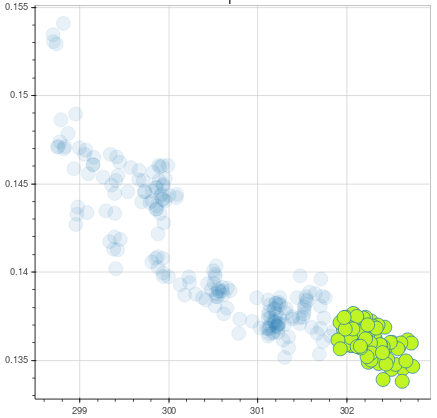
\includegraphics[width=0.9\linewidth]{figures/unsupervised/features/assm-16/u235-fiss/mean-std/mgxs-3}
  \caption{}
  \label{fig:chap10-fiss-mean-std-mgxs-3}
\end{subfigure}
\caption[Clustering of U-235 fission MGXS standard deviations]{Scatter plots of the pin-wise U-235 fission (group 2 of 2) \ac{MGXS} means ($x$) and standard deviations ($y$) for the 1.6\% enriched fuel assembly.}
\label{fig:chap10-fiss-mean-std}
\end{figure}

\clearpage

\begin{figure}[h!]
\centering
\begin{subfigure}{0.45\textwidth}
  \centering
  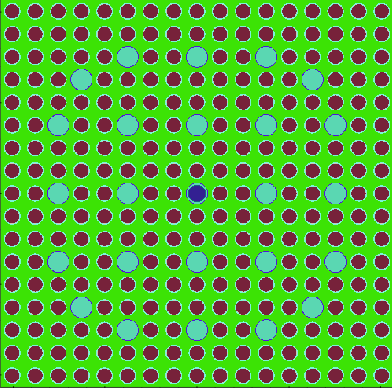
\includegraphics[width=0.9\linewidth]{figures/unsupervised/features/assm-16/geometry}
  \caption{}
  \label{fig:chap10-capt-mean-std-geom}
\end{subfigure}%
\begin{subfigure}{0.45\textwidth}
  \centering
  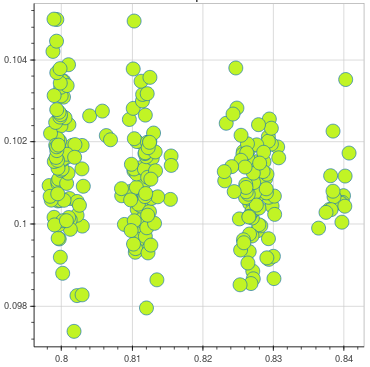
\includegraphics[width=0.9\linewidth]{figures/unsupervised/features/assm-16/u238-capt/mean-std/mgxs}
  \caption{}
  \label{fig:chap10-capt-mean-std-mgxs}
\end{subfigure}
\begin{subfigure}{0.45\textwidth}
  \centering
  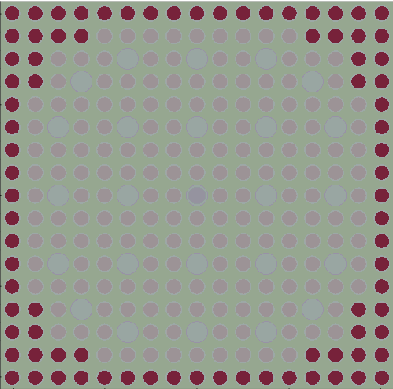
\includegraphics[width=0.9\linewidth]{figures/unsupervised/features/assm-16/u238-capt/mean-std/geometry-2}
  \caption{}
  \label{fig:chap10-capt-mean-std-geom-2}
\end{subfigure}%
\begin{subfigure}{0.45\textwidth}
  \centering
  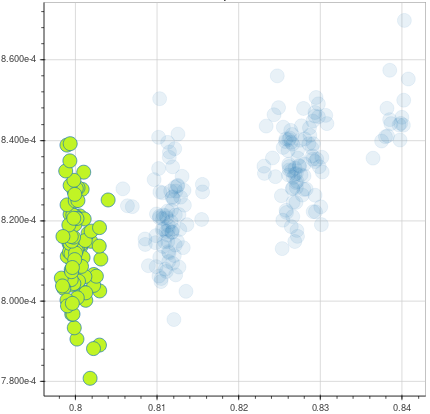
\includegraphics[width=0.9\linewidth]{figures/unsupervised/features/assm-16/u238-capt/mean-std/mgxs-2}
  \caption{}
  \label{fig:chap10-capt-mean-std-mgxs-2}
\end{subfigure}
\begin{subfigure}{0.45\textwidth}
  \centering
  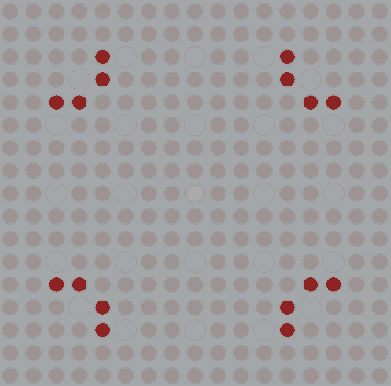
\includegraphics[width=0.9\linewidth]{figures/unsupervised/features/assm-16/u238-capt/mean-std/geometry-3}
  \caption{}
  \label{fig:chap10-capt-mean-std-geom-3}
\end{subfigure}%
\begin{subfigure}{0.45\textwidth}
  \centering
  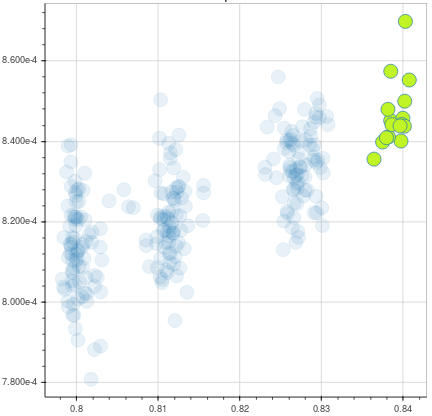
\includegraphics[width=0.9\linewidth]{figures/unsupervised/features/assm-16/u238-capt/mean-std/mgxs-3}
  \caption{}
  \label{fig:chap10-capt-mean-std-mgxs-3}
\end{subfigure}
\caption[Clustering of U-238 capture MGXS standard deviations]{Scatter plots of the pin-wise U-238 capture (group 1 of 2) \ac{MGXS} means ($x$) and standard deviations ($y$) for the 1.6\% enriched fuel assembly.}
\label{fig:chap10-capt-mean-std}
\end{figure}

\clearpage

%%%%%%%%%%%%%%%%%%%%%%%%%%%%%%%%%%
\subsection{Fractional Reactivity}
\label{subsec:chap10-frac-reactivity}

The \textit{fractional reactivity} compares the fission reaction rates for the population of fuel pins in a core geometry. This feature hypothesizes that fuel pins with similar spatial self-shielding effects have similar fission rates. This may be a valid assumption for simple geometries such as fuel assemblies and colorsets with all reflective/periodic \acp{BC}, but may not be true for benchmarks such as \ac{BEAVRS} with large globally-varying power tilts due to leakage. The fission rate statistical uncertainties will necessarily be smaller than those for the microscopic \ac{MGXS} since they are energy-integrated and summed across nuclides. As a result, clustering may emerge from ``noisy'' \ac{MC} fission rate tallies more quickly than is possible for tallies for single energy groups and/or nuclides.

Although the pin-wise fission rates may used directly as a feature, the \textit{i}\ac{MGXS} implementation in this thesis normalizes the pin-wise fission rates to the globally-integrated absorption rate in the fuel as follows:

\begin{equation}
\label{eqn:chap10-frac-reactivity}
\hat{\alpha}_{k} = \frac{\displaystyle\sum\limits_{g=1}^{G}\nu\hat{\Sigma}_{f,i,k,g}\hat{\phi}_{k,g}}{\displaystyle\sum\limits_{k=1}^{K}\displaystyle\sum\limits_{g=1}^{G}\hat{\Sigma}_{a,i,k,g}\hat{\phi}_{k,g}} \times 10^{5}
\end{equation}

\noindent The normalized fractional reactivity $\hat{\alpha}_{k}$  is multiplied by 10$^{5}$ so that it may be reported in the familiar reactivity units of per cent mille (pcm)\footnote{It might be preferable to equivalently normalize the fission rates to the mean. The normalization factor is a matter of analyst preference and does not impact the predictions made by statistical clustering algorithms if the features are standardized as discussed in Sec.~\ref{subsec:chap10-feature-standardize}.}. It is important to note that the denominator in Eqn.~\ref{eqn:chap10-frac-reactivity} encompasses all fuel pins of all compositions (\textit{e.g.}, enrichments) in the core geometry, but does not include absorption in the moderator, clad, \acp{BP}, etc. As a result, the fractional reactivity as defined by this thesis is not indicative of the global reactivity, but rather the reactivity restricted to the fuel.

The fractional reactivity feature is illustrated with scatter plots in Figs.~\ref{fig:chap10-fiss-mean-pcm} and~\ref{fig:chap10-capt-mean-pcm} for 2-group U-235 fission and U-238 capture \ac{MGXS} data, respectively. The scatter plots include a single data point for each of the 264 fuel pins in the 1.6\% enriched fuel assembly benchmark. The $x$ and $y$ coordinates correspond to the tallied \ac{MGXS} means $\hat{\sigma}_{x,i,k,g}$ and normalized fractional reactivities $\hat{\alpha}_{k}$ in units of barns and \ac{pcm}, respectively. The complete datasets are illustrated in Figs.~\ref{fig:chap10-fiss-mean-pcm-mgxs} and~\ref{fig:chap10-capt-mean-pcm-mgxs}. The interactive \textit{i}\ac{MGXS} visualization tool was used to select clusters of \ac{MGXS} and plot the geometry to indicate the associated fuel pins, as displayed in Figs.~\Crefrange{fig:chap10-fiss-mean-pcm-geom-2}{fig:chap10-fiss-mean-pcm-mgxs-3} and~\Crefrange{fig:chap10-capt-mean-pcm-geom-2}{fig:chap10-capt-mean-pcm-mgxs-3} for the fission and capture \ac{MGXS}, respectively. 

The scatter plots illustrate the highly linear relationship between the U-235 fission \ac{MGXS} and fractional reactivities; those pins facially and corner adjacent to distinct \acp{CRGT} have both the largest fission \ac{MGXS} and fission rates due to the differential moderation of the neighboring \acp{CRGT} (at least for this benchmark). The clustering of U-238 capture \ac{MGXS} generally indicates a similar proportional relationship with fractional reactivity. Perhaps more importantly, Fig.~\ref{fig:chap10-capt-mean-pcm} also makes it possible to distinguish ``sub-clusters'' within each of the four primary clusters of U-238 capture \ac{MGXS}. Although the sub-clusters within a primary cluster have similar \ac{MGXS}\footnote{The track density-weighted average \ac{MGXS} for the sub-clusters would be relatively similar.}, there is some variation due to subtle differences in the spatial self-shielding experienced by the pins in the primary cluster.

The visualizations highlight the \textit{hierarchical} nature of spatial self-shielding effects: some factors are most important and induce primary clusters (\textit{i.e.}, whether a fuel pin is adjacent to zero, one or two \acp{CRGT}), while other factors are less consequential yet still induce sub-clusters (\textit{i.e.}, the type adjacency of neighboring \acp{CRGT}). The hierarchy of spatial self-shielding effects will grow increasingly intricate with the size and complexity of the reactor configuration, further motivating the importance for an unsupervised methodology like \textit{i}\ac{MGXS} to identify \ac{MGXS} clustering for arbitrary core geometries.

\begin{figure}[h!]
\centering
\begin{subfigure}{0.45\textwidth}
  \centering
  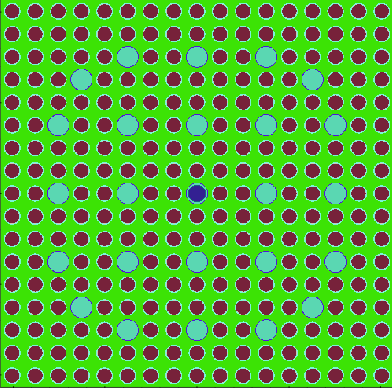
\includegraphics[width=0.9\linewidth]{figures/unsupervised/features/assm-16/geometry}
  \caption{}
  \label{fig:chap10-fiss-mean-pcm-geom}
\end{subfigure}%
\begin{subfigure}{0.45\textwidth}
  \centering
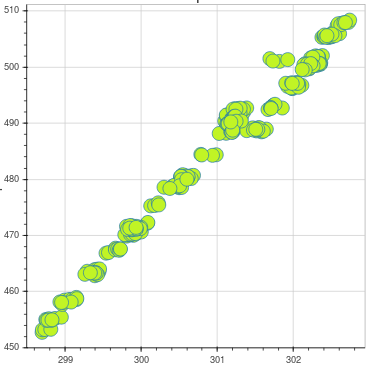
\includegraphics[width=0.9\linewidth]{figures/unsupervised/features/assm-16/u235-fiss/mean-pcm/mgxs}
  \caption{}
  \label{fig:chap10-fiss-mean-pcm-mgxs}
\end{subfigure}
\begin{subfigure}{0.45\textwidth}
  \centering
  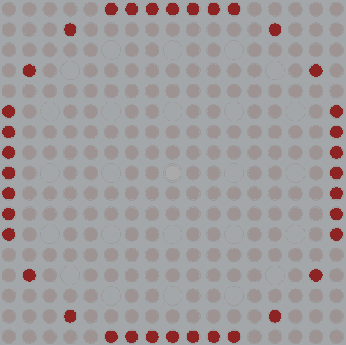
\includegraphics[width=0.9\linewidth]{figures/unsupervised/features/assm-16/u235-fiss/mean-pcm/geometry-2}
  \caption{}
  \label{fig:chap10-fiss-mean-pcm-geom-2}
\end{subfigure}%
\begin{subfigure}{0.45\textwidth}
  \centering
  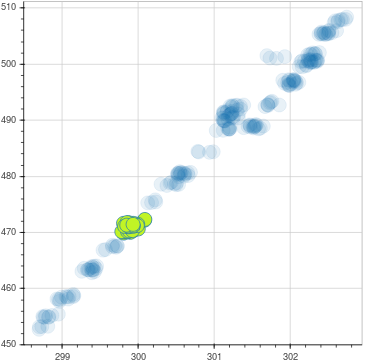
\includegraphics[width=0.9\linewidth]{figures/unsupervised/features/assm-16/u235-fiss/mean-pcm/mgxs-2}
  \caption{}
  \label{fig:chap10-fiss-mean-pcm-mgxs-2}
\end{subfigure}
\begin{subfigure}{0.45\textwidth}
  \centering
  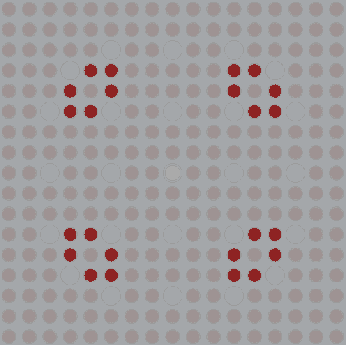
\includegraphics[width=0.9\linewidth]{figures/unsupervised/features/assm-16/u235-fiss/mean-pcm/geometry-3}
  \caption{}
  \label{fig:chap10-fiss-mean-pcm-geom-3}
\end{subfigure}%
\begin{subfigure}{0.45\textwidth}
  \centering
  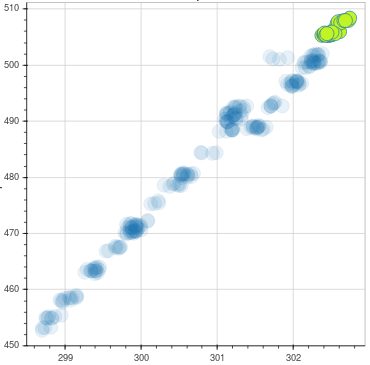
\includegraphics[width=0.9\linewidth]{figures/unsupervised/features/assm-16/u235-fiss/mean-pcm/mgxs-3}
  \caption{}
  \label{fig:chap10-fiss-mean-pcm-mgxs-3}
\end{subfigure}
\caption[Clustering of U-235 fission MGXS fractional reactivities]{Scatter plots of the pin-wise U-235 fission (group 2 of 2) \ac{MGXS} means ($x$) and fractional reactivities ($y$) for the 1.6\% enriched fuel assembly.}
\label{fig:chap10-fiss-mean-pcm}
\end{figure}

\clearpage

\begin{figure}[h!]
\centering
\begin{subfigure}{0.45\textwidth}
  \centering
  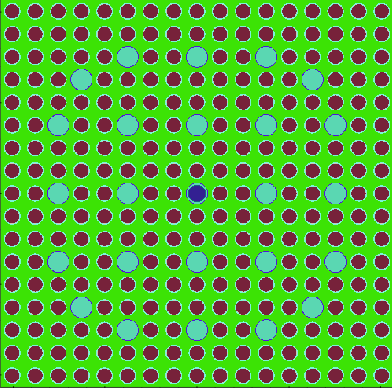
\includegraphics[width=0.9\linewidth]{figures/unsupervised/features/assm-16/geometry}
  \caption{}
  \label{fig:chap10-capt-mean-pcm-geom}
\end{subfigure}%
\begin{subfigure}{0.45\textwidth}
  \centering
  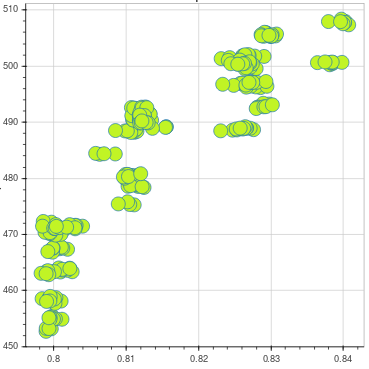
\includegraphics[width=0.9\linewidth]{figures/unsupervised/features/assm-16/u238-capt/mean-pcm/mgxs}
  \caption{}
  \label{fig:chap10-capt-mean-pcm-mgxs}
\end{subfigure}
\begin{subfigure}{0.45\textwidth}
  \centering
  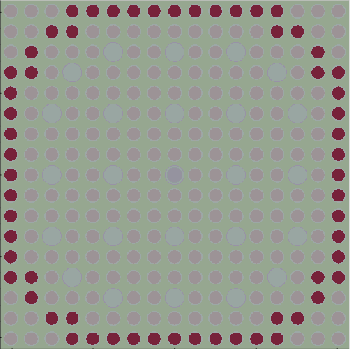
\includegraphics[width=0.9\linewidth]{figures/unsupervised/features/assm-16/u238-capt/mean-pcm/geometry-2}
  \caption{}
  \label{fig:chap10-capt-mean-pcm-geom-2}
\end{subfigure}%
\begin{subfigure}{0.45\textwidth}
  \centering
  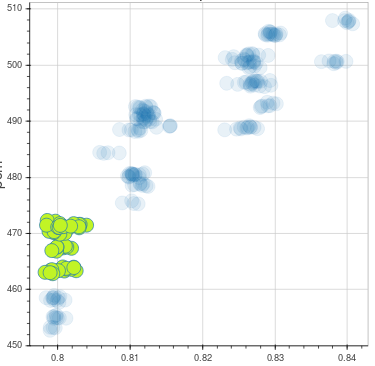
\includegraphics[width=0.9\linewidth]{figures/unsupervised/features/assm-16/u238-capt/mean-pcm/mgxs-2}
  \caption{}
  \label{fig:chap10-capt-mean-pcm-mgxs-2}
\end{subfigure}
\begin{subfigure}{0.45\textwidth}
  \centering
  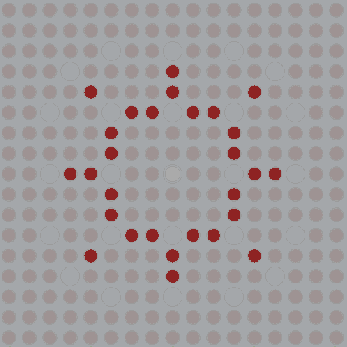
\includegraphics[width=0.9\linewidth]{figures/unsupervised/features/assm-16/u238-capt/mean-pcm/geometry-3}
  \caption{}
  \label{fig:chap10-capt-mean-pcm-geom-3}
\end{subfigure}%
\begin{subfigure}{0.45\textwidth}
  \centering
  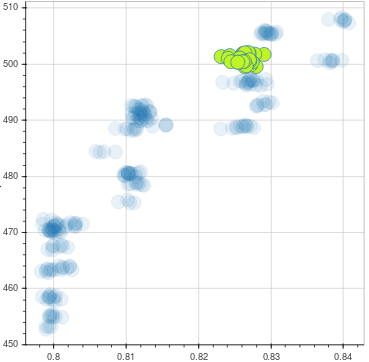
\includegraphics[width=0.9\linewidth]{figures/unsupervised/features/assm-16/u238-capt/mean-pcm/mgxs-3}
  \caption{}
  \label{fig:chap10-capt-mean-pcm-mgxs-3}
\end{subfigure}
\caption[Clustering of U-238 capture MGXS fractional reactivities]{Scatter plots of the pin-wise U-238 capture (group 1 of 2) \ac{MGXS} means ($x$) and fractional reactivities ($y$) for the 1.6\% enriched fuel assembly.}
\label{fig:chap10-capt-mean-pcm}
\end{figure}

\clearpage

%%%%%%%%%%%%%%%%%%%%%%%%%%%	
\subsection{Spectral Index}
\label{subsec:chap10-spec-index}

The \textit{spectral index} compares the ratio of energy-integrated U-238 capture to U-235 fission reaction rates in each fuel pin. The \textit{i}\ac{MGXS} implementation in this thesis computes spectral indices as follows:

\begin{equation}
\label{eqn:chap10-spec-index-u238-capt}
\hat{\beta}_{k} = \frac{\displaystyle\sum\limits_{g=1}^{G}\hat{\sigma}_{\gamma,k,g}^{238}\hat{\phi}_{k,g}}{\displaystyle\sum\limits_{g=1}^{G}\hat{\sigma}_{f,k,g}^{235}\hat{\phi}_{k,g}}
\end{equation}

\noindent where $\hat{\sigma}_{\gamma,k,g}^{238}$ and $\hat{\sigma}_{f,k,g}^{235}$ are the microscopic U-238 radiative capture and U-235 fission production \ac{MGXS} for fuel pin instance $k$ and energy group $g$, respectively\footnote{The U-235 fission and fission production \ac{MGXS} may be used interchangeably in Eqn.~\ref{eqn:chap10-spec-index-u238-capt} with no impact on the predictions made by unsupervised statistical clustering algorithms.}. This feature postulates that the capture-to-fission ratio will significantly vary for fuel pins and energy groups with different spatial self-shielding effects. The spectral index is especially relevant since it accounts for relative differences in the U-238 capture rates, which previous chapters showed can only be accurately computed if an appropriate pin-wise spatial homogenization scheme is used. Unlike the fractional reactivity, the spectral index may identify pins with similar flux shapes but very different flux magnitudes since it is the ratio of two pin-wise reaction rates.

The spectral index feature is illustrated with scatter plots in Figs.~\ref{fig:chap10-fiss-mean-spect-ind} and~\ref{fig:chap10-capt-mean-spect-ind} for 2-group U-235 fission and U-238 capture \ac{MGXS} data, respectively. The scatter plots include a single data point for each of the 264 fuel pins in the 1.6\% enriched fuel assembly benchmark. The $x$ and $y$ coordinates correspond to the tallied \ac{MGXS} means $\hat{\sigma}_{x,i,k,g}$ and spectral indices $\hat{\beta}_{k}$, respectively. The complete datasets are illustrated in Figs.~\ref{fig:chap10-fiss-mean-spect-ind-mgxs} and~\ref{fig:chap10-capt-mean-spect-ind-mgxs}. The interactive \textit{i}\ac{MGXS} visualization tool was used to select clusters of \ac{MGXS} and plot the geometry to indicate the associated fuel pins, as displayed in Figs.~\Crefrange{fig:chap10-fiss-mean-spect-ind-geom-2}{fig:chap10-fiss-mean-spect-ind-mgxs-3} and~\Crefrange{fig:chap10-capt-mean-spect-ind-geom-2}{fig:chap10-capt-mean-spect-ind-mgxs-3} for the fission and capture \ac{MGXS}, respectively. 

\begin{figure}[h!]
\centering
\begin{subfigure}{0.42\textwidth}
  \centering
  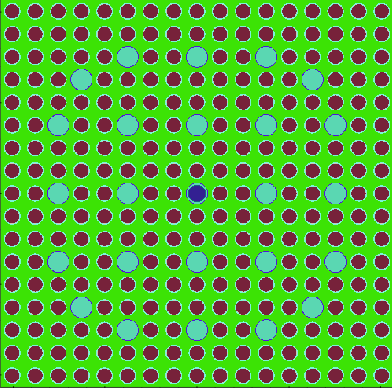
\includegraphics[width=0.8\linewidth]{figures/unsupervised/features/assm-16/geometry}
  \caption{}
  \label{fig:chap10-fiss-mean-spect-ind-geom}
\end{subfigure}%
\begin{subfigure}{0.45\textwidth}
  \centering
  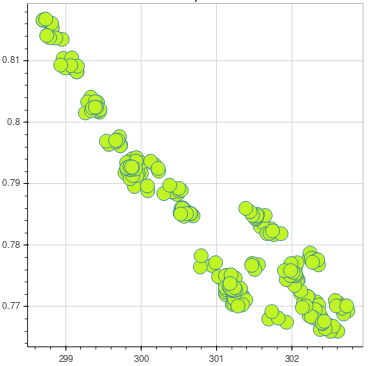
\includegraphics[width=0.9\linewidth]{figures/unsupervised/features/assm-16/u235-fiss/mean-spect-ind-sum/mgxs}
  \caption{}
  \label{fig:chap10-fiss-mean-spect-ind-mgxs}
\end{subfigure}
\begin{subfigure}{0.45\textwidth}
  \centering
  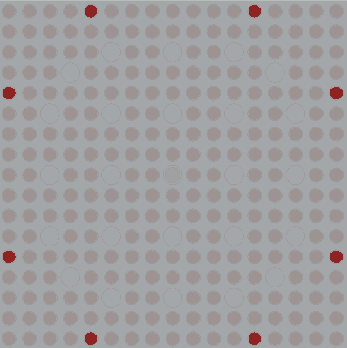
\includegraphics[width=0.9\linewidth]{figures/unsupervised/features/assm-16/u235-fiss/mean-spect-ind-sum/geometry-2}
  \caption{}
  \label{fig:chap10-fiss-mean-spect-ind-geom-2}
\end{subfigure}%
\begin{subfigure}{0.45\textwidth}
  \centering
  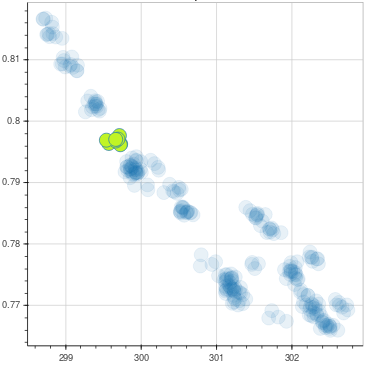
\includegraphics[width=0.9\linewidth]{figures/unsupervised/features/assm-16/u235-fiss/mean-spect-ind-sum/mgxs-2}
  \caption{}
  \label{fig:chap10-fiss-mean-spect-ind-mgxs-2}
\end{subfigure}
\begin{subfigure}{0.45\textwidth}
  \centering
  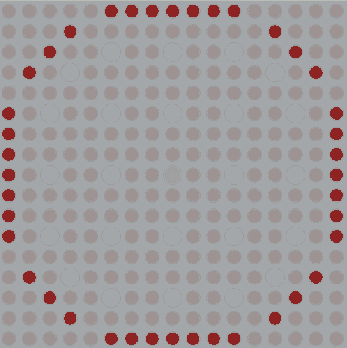
\includegraphics[width=0.9\linewidth]{figures/unsupervised/features/assm-16/u235-fiss/mean-spect-ind-sum/geometry-3}
  \caption{}
  \label{fig:chap10-fiss-mean-spect-ind-geom-3}
\end{subfigure}%
\begin{subfigure}{0.45\textwidth}
  \centering
  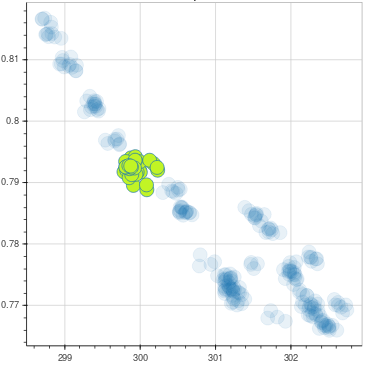
\includegraphics[width=0.9\linewidth]{figures/unsupervised/features/assm-16/u235-fiss/mean-spect-ind-sum/mgxs-3}
  \caption{}
  \label{fig:chap10-fiss-mean-spect-ind-mgxs-3}
\end{subfigure}
\caption[Clustering of U-235 fission MGXS spectral indices]{Scatter plots of the pin-wise U-235 fission (group 2 of 2) \ac{MGXS} means ($x$) and spectral indices ($y$) for the 1.6\% enriched fuel assembly.}
\label{fig:chap10-fiss-mean-spect-ind}
\end{figure}

%\clearpage

\begin{figure}[h!]
\centering
\begin{subfigure}{0.45\textwidth}
  \centering
  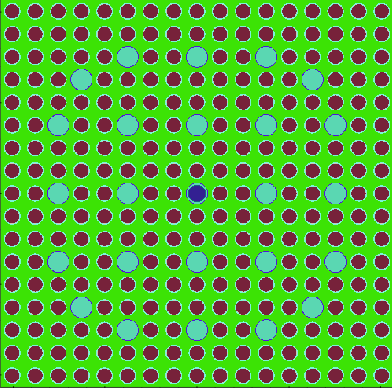
\includegraphics[width=0.9\linewidth]{figures/unsupervised/features/assm-16/geometry}
  \caption{}
  \label{fig:chap10-capt-mean-spect-ind-geom}
\end{subfigure}%
\begin{subfigure}{0.45\textwidth}
  \centering
  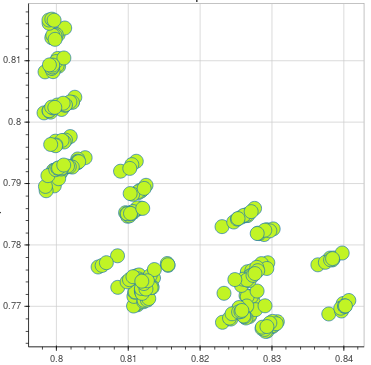
\includegraphics[width=0.9\linewidth]{figures/unsupervised/features/assm-16/u238-capt/mean-spect-ind-sum/mgxs}
  \caption{}
  \label{fig:chap10-capt-mean-spect-ind-mgxs}
\end{subfigure}
\begin{subfigure}{0.45\textwidth}
  \centering
  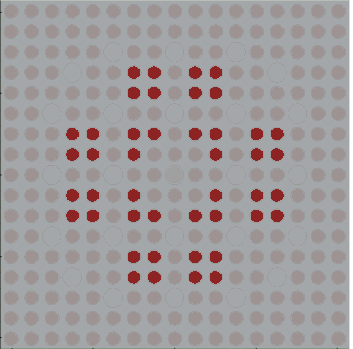
\includegraphics[width=0.9\linewidth]{figures/unsupervised/features/assm-16/u238-capt/mean-spect-ind-sum/geometry-2}
  \caption{}
  \label{fig:chap10-capt-mean-spect-ind-geom-2}
\end{subfigure}%
\begin{subfigure}{0.45\textwidth}
  \centering
  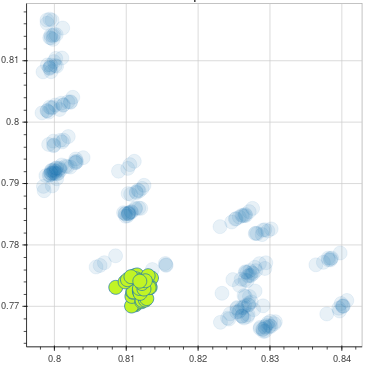
\includegraphics[width=0.9\linewidth]{figures/unsupervised/features/assm-16/u238-capt/mean-spect-ind-sum/mgxs-2}
  \caption{}
  \label{fig:chap10-capt-mean-spect-ind-mgxs-2}
\end{subfigure}
\begin{subfigure}{0.45\textwidth}
  \centering
  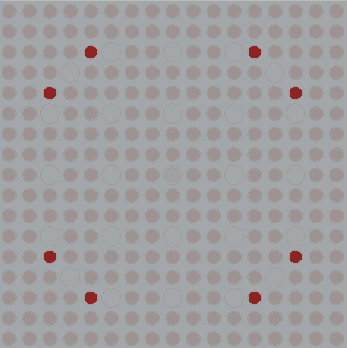
\includegraphics[width=0.9\linewidth]{figures/unsupervised/features/assm-16/u238-capt/mean-spect-ind-sum/geometry-3}
  \caption{}
  \label{fig:chap10-capt-mean-spect-ind-geom-3}
\end{subfigure}%
\begin{subfigure}{0.45\textwidth}
  \centering
  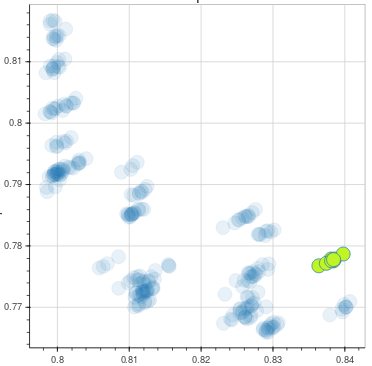
\includegraphics[width=0.9\linewidth]{figures/unsupervised/features/assm-16/u238-capt/mean-spect-ind-sum/mgxs-3}
  \caption{}
  \label{fig:chap10-capt-mean-spect-ind-mgxs-3}
\end{subfigure}
\caption[Clustering of U-238 capture MGXS spectral indices]{Scatter plots of the pin-wise U-238 capture (group 1 of 2) \ac{MGXS} means ($x$) and spectral indices ($y$) for the 1.6\% enriched fuel assembly.}
\label{fig:chap10-capt-mean-spect-ind}
\end{figure}

%\clearpage

The figures illustrate a complex relationship between the U-235 fission \ac{MGXS} and the spectral indices. In contrast to the fractional reactivity, both the fission and capture \ac{MGXS} are negatively correlated with the spectral index. In particular, the more differential moderation from neighboring \acp{CRGT}, the smaller the spectral index. Although the capture and fission rates both increase with differential moderation, these scatter plots indicate that U-235 fission increases \textit{faster} than U-238 capture. In addition, the clusters are more spread out than the more linear trends observed for the fractional reactivities. The scatter plots indicate that the spectral index is potentially more effective at separating sub-clusters within each primary cluster than fractional reactivity.

%(at least for this benchmark). 


%%%%%%%%%%%%%%%%%%%%%%%%%%%%%
\subsection{Nuclide Fraction}
\label{subsec:chap10-nuclide-frac}

The fractional reactivity and spectral index are both energy-integrated features, the \textit{nuclide fraction} feature is specific to each energy group. The nuclide fraction is defined as the ratio of each pin-wise microscopic \ac{MGXS} $\hat{\sigma}_{x,i,k,g}$ for reaction $x$, nuclide $i$ and energy group $k$ to the total \ac{MGXS} for the $\hat{\sigma}_{t,i,k,g}$ corresponding nuclide and energy group:

\begin{equation}
\label{eqn:chap10-nuclide-frac}
\hat{\tau}_{x,i,k,g} = \frac{\hat{\sigma}_{x,i,k,g}}{\hat{\sigma}_{t,i,k,g}}
\end{equation}

The nuclide fraction feature $\hat{\tau}_{x,i,k,g}$ is motivated by the hypothesis that spatial self-shielding effects may disproportionately impact certain reaction types (\textit{e.g.}, U-238 capture) more than the total \ac{MGXS}. Since the nuclide fraction is computed for each energy group, it may be more challenging to identify clusters with this feature with ``noisy'' \ac{MC} tally data than may be the case for the energy-integrated fractional reactivity and spectral index features. Like the spectral index, the nuclide fraction may identify pins with similar flux shapes but very different flux magnitudes since it is the ratio of two pin-wise reaction rates.

\begin{figure}[h!]
\centering
\begin{subfigure}{0.45\textwidth}
  \centering
  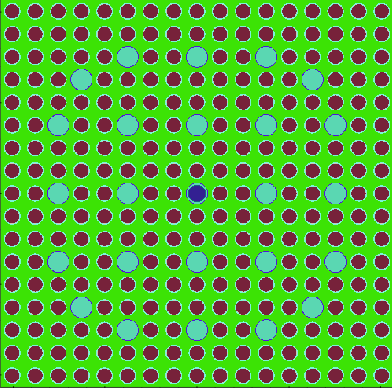
\includegraphics[width=0.9\linewidth]{figures/unsupervised/features/assm-16/geometry}
  \caption{}
  \label{fig:chap10-fiss-mean-nuc-frac-geom}
\end{subfigure}%
\begin{subfigure}{0.45\textwidth}
  \centering
  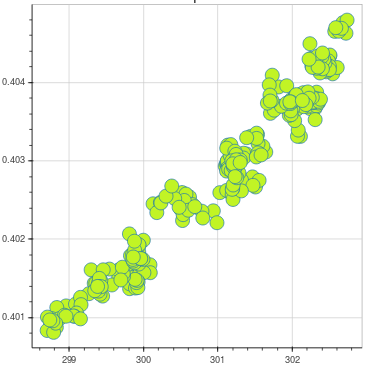
\includegraphics[width=0.9\linewidth]{figures/unsupervised/features/assm-16/u235-fiss/mean-nuc-frac/mgxs}
  \caption{}
  \label{fig:chap10-fiss-mean-nuc-frac-mgxs}
\end{subfigure}
\begin{subfigure}{0.45\textwidth}
  \centering
  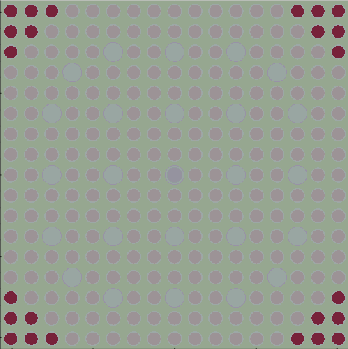
\includegraphics[width=0.9\linewidth]{figures/unsupervised/features/assm-16/u235-fiss/mean-nuc-frac/geometry-2}
  \caption{}
  \label{fig:chap10-fiss-mean-nuc-frac-geom-2}
\end{subfigure}%
\begin{subfigure}{0.45\textwidth}
  \centering
  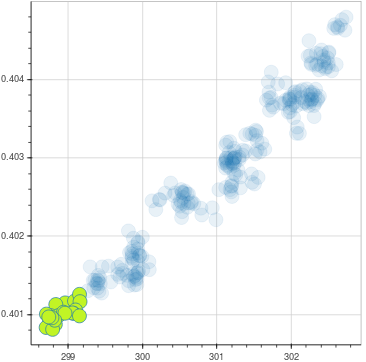
\includegraphics[width=0.9\linewidth]{figures/unsupervised/features/assm-16/u235-fiss/mean-nuc-frac/mgxs-2}
  \caption{}
  \label{fig:chap10-fiss-mean-nuc-frac-mgxs-2}
\end{subfigure}
\begin{subfigure}{0.45\textwidth}
  \centering
  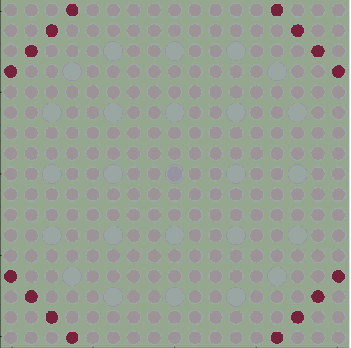
\includegraphics[width=0.9\linewidth]{figures/unsupervised/features/assm-16/u235-fiss/mean-nuc-frac/geometry-3}
  \caption{}
  \label{fig:chap10-fiss-mean-nuc-frac-geom-3}
\end{subfigure}%
\begin{subfigure}{0.45\textwidth}
  \centering
  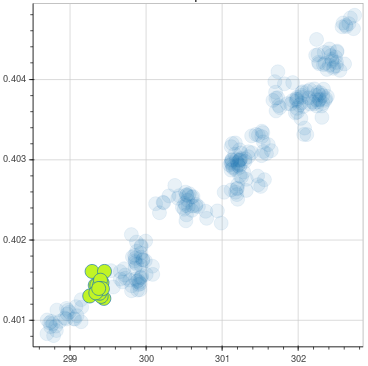
\includegraphics[width=0.9\linewidth]{figures/unsupervised/features/assm-16/u235-fiss/mean-nuc-frac/mgxs-3}
  \caption{}
  \label{fig:chap10-fiss-mean-nuc-frac-mgxs-3}
\end{subfigure}
\caption[Clustering of U-235 fission MGXS nuclide fractions]{Scatter plots of the pin-wise U-235 fission (group 2 of 2) \ac{MGXS} means ($x$) and nuclide fractions ($y$) for the 1.6\% enriched fuel assembly.}
\label{fig:chap10-fiss-mean-nuc-frac}
\end{figure}

%\clearpage

\begin{figure}[h!]
\centering
\begin{subfigure}{0.45\textwidth}
  \centering
  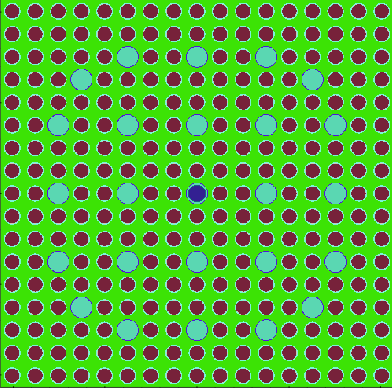
\includegraphics[width=0.9\linewidth]{figures/unsupervised/features/assm-16/geometry}
  \caption{}
  \label{fig:chap10-capt-mean-nuc-frac-geom}
\end{subfigure}%
\begin{subfigure}{0.45\textwidth}
  \centering
  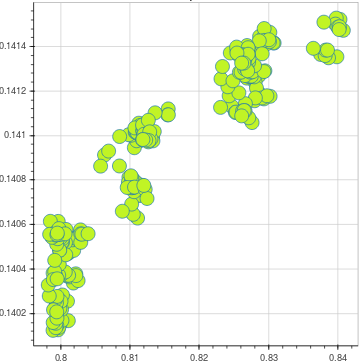
\includegraphics[width=0.9\linewidth]{figures/unsupervised/features/assm-16/u238-capt/mean-nuc-frac/mgxs}
  \caption{}
  \label{fig:chap10-capt-mean-nuc-frac-mgxs}
\end{subfigure}
\begin{subfigure}{0.45\textwidth}
  \centering
  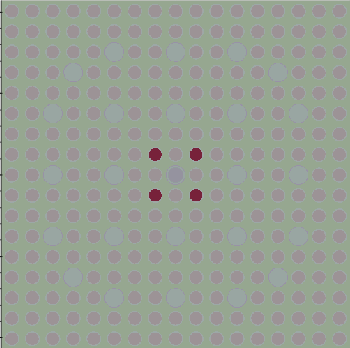
\includegraphics[width=0.9\linewidth]{figures/unsupervised/features/assm-16/u238-capt/mean-nuc-frac/geometry-2}
  \caption{}
  \label{fig:chap10-capt-mean-nuc-frac-geom-2}
\end{subfigure}%
\begin{subfigure}{0.45\textwidth}
  \centering
  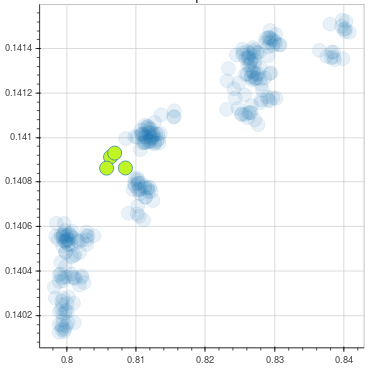
\includegraphics[width=0.9\linewidth]{figures/unsupervised/features/assm-16/u238-capt/mean-nuc-frac/mgxs-2}
  \caption{}
  \label{fig:chap10-capt-mean-nuc-frac-mgxs-2}
\end{subfigure}
\begin{subfigure}{0.45\textwidth}
  \centering
  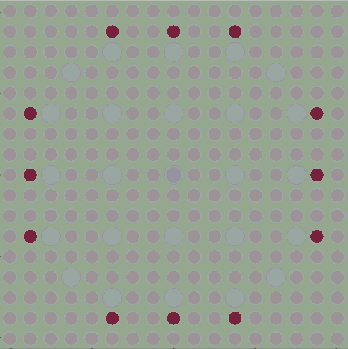
\includegraphics[width=0.9\linewidth]{figures/unsupervised/features/assm-16/u238-capt/mean-nuc-frac/geometry-3}
  \caption{}
  \label{fig:chap10-capt-mean-nuc-frac-geom-3}
\end{subfigure}%
\begin{subfigure}{0.45\textwidth}
  \centering
  \includegraphics[width=0.9\linewidth]{figures/unsupervised/features/assm-16/u238-capt/mean-nuc-frac/mgxs-3}
  \caption{}
  \label{fig:chap10-capt-mean-nuc-frac-mgxs-3}
\end{subfigure}
\caption[Clustering of U-238 capture MGXS nuclide fractions]{Scatter plots of the pin-wise U-238 capture (group 1 of 2) \ac{MGXS} means ($x$) and nuclide fractions ($y$) for the 1.6\% enriched fuel assembly.}
\label{fig:chap10-capt-mean-nuc-frac}
\end{figure}

%\clearpage

The nuclide fraction feature is illustrated with scatter plots in Figs.~\ref{fig:chap10-fiss-mean-nuc-frac} and~\ref{fig:chap10-capt-mean-nuc-frac} for 2-group U-235 fission and U-238 capture \ac{MGXS} data, respectively. The scatter plots include a single data point for each of the 264 fuel pins in the 1.6\% enriched fuel assembly benchmark. The $x$ and $y$ coordinates correspond to the tallied \ac{MGXS} means $\hat{\sigma}_{x,i,k,g}$ and nuclide fractions $\beta_{k}$, respectively. The complete datasets are illustrated in Figs.~\ref{fig:chap10-fiss-mean-nuc-frac-mgxs} and~\ref{fig:chap10-capt-mean-nuc-frac-mgxs}. The interactive \textit{i}\ac{MGXS} visualization tool was used to select clusters of \ac{MGXS} and plot the geometry to indicate the associated fuel pins, as displayed in Figs.~\Crefrange{fig:chap10-fiss-mean-nuc-frac-geom-2}{fig:chap10-fiss-mean-nuc-frac-mgxs-3} and~\Crefrange{fig:chap10-capt-mean-nuc-frac-geom-2}{fig:chap10-capt-mean-nuc-frac-mgxs-3} for the fission and capture \ac{MGXS}, respectively. 

The figures illustrate a positive correlation between both the U-235 fission and U-238 capture \ac{MGXS} and the nuclide fractions (at least for this benchmark). In particular, the more differential moderation from neighboring \acp{CRGT}, the smaller the larger the nuclide fraction. Although the fission, capture and total rates all increase with differential moderation, these scatter plots indicate that U-235 fission and U-238 capture increases \textit{faster} than the corresponding total reaction rates with U-235 and U-238. The clusters are more spread out than the more linear trends observed for the fractional reactivities, but this is likely due to the relatively larger statistical uncertainty for the energy-specific nuclide fractions than the energy-integrated fractional reactivities.

%%%%%%%%%%%%%%%%%%%%%%%%%%%%
%\subsection{Total Fraction}
%\label{subsec:chap10-tot-frac}
%
%first paragraph: explain what it is
%-divide pin-wise micro \ac{MGXS} for each nuclide/reaction/group by the corresponding total \ac{MGXS} for that nuclide/reaction/group trio
%-Eqn.~\ref{eqn:chap10-tot-frac}
%-explain what it indicates...???
%-note that $I$ designates the total number of nuclides in a fuel pin
%
%\begin{equation}
%\label{eqn:chap10-tot-frac}
%\omega_{x,i,k,g} = \frac{\hat{\sigma}_{x,i,k,g}}{\displaystyle\sum\limits_{i=1}^{I}\hat{\sigma}_{t,i,k,g}}
%\end{equation}

%%%%%%%%%%%%%%%%%%%%%%%%%%%%%%%%%%%%
\subsection{Feature Standardization}
\label{subsec:chap10-feature-standardize}

Each of the features described in the preceding sections is assembled into feature vectors for each sample as illustrated in Fig.~\ref{fig:chap10-features-example}. From a practical standpoint, the \textit{i}\ac{MGXS} implementation in this thesis represents the sample feature vectors with a 2D \texttt{DataFrame} object from the Pandas module~\cite{mckinney2010pandas} for data processing in Python. Each column in the \texttt{DataFrame} corresponds to a feature, and each row corresponds to a sample. This \texttt{DataFrame} is the input to the feature selection stage of the \textit{i}\ac{MGXS} pipeline. However, each feature must first be \textit{standardized} before used as an input to a predictive model.

\begin{figure}[h!]
\centering
\includegraphics[width=0.95\linewidth]{figures/unsupervised/features/engineering/features}
\vspace{2mm}
\caption[Example \textit{i}MGXS sample feature vectors]{\textit{i}\ac{MGXS} feature extraction computes fractional reactivities $\hat{\alpha}_{k}$, spectral indices $\hat{\beta}_{k}$, nuclide fractions $\hat{\tau}_{x,i,k,g}$, \ac{MGXS} means $\hat{\sigma}_{x,i,k,g}$ and standard deviations $\sigma_{\hat{\sigma}_{x,i,k,g}}$.}
\label{fig:chap10-features-example}
\end{figure}

Feature standardization -- also known as \textit{mean removal} and/or \textit{variance scaling} -- is commonly needed since many machine learning estimators assume that all features are centered about zero with near unit variance. In the context of \textit{i}\ac{MGXS}, the distance between samples (or clusters) in feature space will be skewed if the features are not standardized. In particular, the distance will be dominated by features with the largest magnitudes (\textit{e.g.}, thermal U-235 fission \ac{MGXS}), and conversely, insensitive to features with small magnitudes (\textit{e.g.}, \ac{MGXS} standard deviations). The canonical form of standardization \textit{translates} each sample by subtracting the mean $\overline{\hat{f}_{j}}$, and \textit{scales} each sample by dividing by the standard deviation $\sigma_{\hat{f}_{j}}$ of feature $j$:

\begin{equation}
\label{eqn:chap10-standard-standardize}
\hat{f}_{j,k}^{*} = \frac{\hat{f}_{j,k} - \overline{\hat{f}_{j}}}{\sigma_{\hat{f}_{j}}}
\end{equation}

\noindent where $\hat{f}_{j,k}^{*}$ is the standardized feature $j$ for fuel pin instance $k$. Several standardization schemes are provided by the \texttt{sklearn.preprocessing} module of the \texttt{scikit-learn} Python package for machine learning~\cite{pedregosa2011sklearn}. The \textit{i}\ac{MGXS} implementation in this thesis uses the \texttt{RobustScaler} to subtract the median and divide by the interquartile range (IQR)\footnote{The interquartile range is the difference between the first and third quartiles: $\mathrm{IQR} = Q_{3} - Q_{1}$.} to diminish the influence of outliers on the standardization process:

\begin{equation}
\label{eqn:chap10-robust-standardize}
\hat{f}_{j,k}^{*} = \frac{\hat{f}_{j,k} - \mathrm{median}\left\{\hat{f}_{j,1}, \hat{f}_{j,2}, \dots, \hat{f}_{j,K}\right\}}{\mathrm{IQR}_{\hat{f}_{j}}}
\end{equation}

\begin{emphbox}
\textbf{Features are random variables derived from \ac{MC} tally data which may provide information about \ac{MGXS} clustering. Feature vectors are constructed for each fuel pin instance and used as inputs for predictive clustering models.}
\end{emphbox}


%%%%%%%%%%%%%%%%%%%%%%%%%%%%%%%%%%%%%%%%%%%%%%%%%%%%%%%%%%%%%%%%%%%%%%%%%%%%%%%
\section{Feature Selection}
\label{sec:chap10-feature-select}

The \textit{feature selection} stage in the data processing pipeline in Fig.~\ref{fig:chap10-pipeline} determines which features to use when training\footnote{In machine learning, \textit{training} a model refers to the process of assigning numerical values to the parameters of the model to best fit an empirical dataset.} a clustering model. The feature extraction stage provides many different features, some of which may be poor predictors of \ac{MGXS} clusters. In addition, some features may be highly correlated and redundant as input variables to a predictive model. Feature selection attempts to identify the smallest possible subset of features necessary to achieve the desired predictive accuracy. Feature selection plays an important role in balancing the canonical \textit{bias--variance tradeoff} in statistics and machine learning by reducing model variance, while potentially increasing model bias. In particular, feature selection is used to train simple(r) machine learning models for the following three reasons:

\begin{itemize}[noitemsep]
\item \textbf{Reduce Model Complexity} -- Simpler models are easier to intuit and explain
\item \textbf{Reduce Generalization Error} -- Simpler models reduce the risk of over-fitting
\item \textbf{Reduce Training Time} -- Simpler models are computationally efficient to train
\end{itemize}

Automated feature selection methods are often classified into three main categories: \textit{filter}, \textit{wrapper}, and \textit{embedded} methods. \textit{Filter methods} are agnostic to the family of predictive models one wishes to train and selects features which provide the most information about a target variable. Correlation Feature Selection~\cite{hall1999correlation} is an example of a filter method which searches for the smallest subset of features which are highly correlated with the target variable, but uncorrelated with each other. In contrast to filter methods, \textit{wrapper methods} evaluate subsets of features to determine their collective ability to minimize the generalization error of some specific family of predictive models. Wrapper methods may be computationally expensive since it entails a search of the space of possible feature subsets. In addition, wrapper methods may be at greater risk of over-fitting than filter methods since the feature selection criteria is based on model accuracy. Finally, \textit{embedded methods} select features as an integral part of the model training procedure. Some examples of embedded methods include $\ell_{1}$-regularization techniques and Recursive Feature Elimination~\cite{guyon2002rfe}. The interested reader is referred to~\cite{guyon2003select} or the plethora of other sources in the literature for more detailed information about automated feature selection methods.

This thesis makes a fairly limited use of feature selection techniques in its implementation of \textit{i}\ac{MGXS}. In particular, a number of relatively simple filter and wrapper methods are presented in the following sections as options to select the best features. This process is illustrated as part of the \textit{i}\ac{MGXS} data processing pipeline in Fig.~\ref{fig:chap10-select}. Sec.~\ref{subsec:chap10-litmus} presents \textit{litmus tests} to filter the features and choose those pairings of nuclides and reaction types which are most likely to exhibit clustering. Sec.~\ref{subsec:chap10-var-threshold} introduces variance thresholding, while Sec.~\ref{subsec:chap10-univariate-selection} highlights a collection of filter methods which select the highest scoring features. Sec.~\ref{subsec:chap10-select-from-model} discusses a wrapper method which selects features based on their importances for decision tree or ensemble regressors. Finally, while domain knowledge is not an automated approach to feature downselection, it is employed by the case studies in the following chapter and is discussed in Sec.~\ref{subsec:chap10-pinch-selection}.

%Sec.~\ref{subsec:chap10-litmus-tot-frac} introduces a threshold-based method to downselect those nuclides with the most relevant data to cluster for a given energy group. Similarly, Sec.~\ref{subsec:chap10-litmus-nuc-frac} presents a threshold for the nuclide fraction to choose the ``best'' reaction type to cluster for a given nuclide and energy group.

\begin{figure}[h!]
\centering
\includegraphics[width=0.95\linewidth]{figures/unsupervised/features/engineering/select}
\vspace{2mm}
\caption[\textit{i}MGXS feature selection]{Feature selection chooses the features used to train a clustering model.}
\label{fig:chap10-select}
\end{figure}

It is important to note that the methods and metrics highlighted here should be considered an exhaustive list of options for feature selection for \textit{i}\ac{MGXS}. Furthermore, while all of the options discussed are supported in the \textit{i}\ac{MGXS} for this thesis, out of practical necessity only a few of the methods are evaluated by the empirical cases studies in this and the following chapter. Future work may aim to provide a more systematic appraisal of various feature selection methods for the \textit{i}\ac{MGXS} pipeline.

%%%%%%%%%%%%%%%%%%%%%%%%%%%%%%%%%%%%%%%%
\subsection{Litmus Tests}
\label{subsec:chap10-litmus}

\textit{Litmus tests} are filter methods specifically designed to select data for particular nuclides and reaction types for clustering. The litmus tests presented here are used to downselect the \ac{MGXS} mean and standard deviation features by predicting which nuclides and reaction types are most likely to exhibit clustering effects. The litmus tests are independently applied to each nuclide / energy group / reaction type grouping. Sec.~\ref{subsubsec:chap10-litmus-tot-frac} introduces total fraction thresholding to select a nuclide for a given energy group, while Sec.~\ref{subsubsec:chap10-litmus-nuc-frac} introduces nuclide fraction thresholding to select a reaction type for a given nuclide and energy group. Sec.~\ref{subsubsec:chap10-litmus-nuc-frac} discusses how normality tests can be used to reject features which may have been drawn from a normal distribution.

%%%%%%%%%%%%%%%%%%%%%%%%%%%%%%%%%%%%%%%%
\subsubsection{Total Fraction Thresholding}
\label{subsubsec:chap10-litmus-tot-frac}

\textit{Total fraction thresholding} is a filter method used to select \ac{MGXS}-based features\footnote{\ac{MGXS}-based features include the microscopic \ac{MGXS} means $\hat{\sigma}_{x,i,k,g}$ and standard deviations $\sigma_{\hat{\sigma}_{x,i,k,g}}$, as well as the nuclide fraction $\hat{\tau}_{x,i,k,g}$.} for one or more nuclides for a particular energy group $g$ and reaction type $x$.
The total fraction gives an indication of how much a particular nuclide contributes to the total \ac{MGXS}. 
The \textit{total fraction} $\hat{\omega}_{x,i,k,g}$ is defined as the ratio of a macroscopic \ac{MGXS} $\hat{\Sigma}_{x,i,k,g}$ for nuclide $i$ and fuel pin instance $k$ to the total macroscopic \ac{MGXS} for all nuclides:

\begin{equation}
\label{eqn:chap10-tot-frac}
\hat{\omega}_{x,i,k,g} = \frac{\hat{\Sigma}_{x,i,k,g}}{\displaystyle\sum\limits_{i=1}^{I}\hat{\Sigma}_{t,i,k,g}}
\end{equation}

The \textit{i}\ac{MGXS} implementation in this thesis simply chooses \ac{MGXS}-based features for nuclide $i$ if the mean $\overline{\hat{\omega}}_{x,i,g}$ across fuel pins is greater than some user-defined threshold. This litmus test assumes that nuclide(s) which contribute little to the total \ac{MGXS} are not important to cluster. This assumption may not always be valid if some small \ac{MGXS} disproportionately reflect spatial self-shielding effects. For example, if the flux is appreciably depressed in narrow resonance groups for nuclides and reaction types which are especially sensitive to spatial self-shielding (\textit{e.g.}, U-238 capture), then the \ac{MGXS} may likewise be depressed such that the total fraction drops below the threshold and the feature(s) are neglected. The case studies explored in the following chapter use a relatively conservative value of 0.1 for the threshold such that \ac{MGXS}-based features for trace nuclides (\textit{e.g.}, O-17, U-234) are neglected while those for U-235 and U-238 are always selected.

%This is unlikely, however, since spatial self-shielding effects are only manifested as clusters in pin-wise \ac{MGXS} if the continuous energy data varies over a relatively large range for a given energy group. A widely varying cross section, such as those in the resonance regime, will most likely result in a relatively large microscopic \ac{MGXS} and total fraction for the nuclide.

%%%%%%%%%%%%%%%%%%%%%%%%%%%%%%%%%%%%%%%%%%
\subsubsection{Nuclide Fraction Thresholding}
\label{subsubsec:chap10-litmus-nuc-frac}

\textit{Nuclide fraction thresholding} is a filter method used to select \ac{MGXS}-based features for one or more reaction types for a particular nuclide $i$ and energy group  $g$ pairing. The nuclide fraction $\hat{\tau}_{x,i,k,g}$ (Eqn.~\ref{eqn:chap10-nuclide-frac}) gives an indication of how much a particular reaction contributes to a nuclide's total \ac{MGXS}. This litmus test is employed in a similar fashion to total fraction thresholding. In particular, the \textit{i}\ac{MGXS} implementation in this thesis simply chooses \ac{MGXS}-based features for nuclide $i$ and reaction $x$ if the mean $\overline{\hat{\tau}}_{x,i,g}$ across fuel pins is greater than some user-defined threshold.

The nuclide fraction thresholding litmus test assumes that reaction(s) which contribute little to a nuclide's total \ac{MGXS} are not important to cluster. As was noted for total fraction thresholding, this assumption may not always be valid if some small \ac{MGXS} disproportionately reflect spatial self-shielding effects. For example, if the flux is appreciably depressed in narrow resonance groups for nuclides and reaction types which are especially sensitive to spatial self-shielding (\textit{e.g.}, U-238 capture), then the \ac{MGXS} may likewise be depressed such that the total fraction drops below the threshold and the feature(s) are neglected. The case studies explored in the following chapter use a relatively conservative value of 0.3 for the threshold such that \ac{MGXS}-based features for U-235 fission and U-238 capture are always selected for thermal energy groups.

%%%%%%%%%%%%%%%%%%%%%%%%%%%%%%%
\subsubsection{Normality Tests}
\label{subsubsec:chap10-litmus-normality}

\textit{Normality tests} select features which fail to satisfy the null hypothesis that the data is drawn from a normal distribution. Normality tests are a filter method for feature selection motivated by the thought experiment posed in Chap.~\ref{chap:spatial} and investigated in Sec.~\ref{subsec:chap9-qq-plots} with \ac{Q-Q} plots. This litmus test assumes that the realizations of a given feature are normally distributed if they do not reflect spatial self-shielding effects. If this assumption is valid, then those features which pass a normality test do not provide any useful information about \ac{MGXS} clustering and can be neglected.

The \textit{i}\ac{MGXS} implementation in this thesis uses the Shapiro-Wilk test of normality~\cite{shapiro1965analysis} computed using the Python \texttt{scipy.stats} package~\cite{jones2011scipy}. The Shapiro-Wilk test is applied to all samples for a given feature to compute a $p$-value to quantify the null hypothesis that the population came from a normal distribution. A user-defined significance level $\alpha$ is chosen (\textit{e.g.}, 0.001) and compared with the Shapiro-Wilk $p$-value. If $p > \alpha$ then the null hypothesis that the feature is normally distributed is accepted and the feature is dropped from the dataset. Alternatively, if $p < \alpha$, then the null hypothesis is rejected and the feature is selected as a potentially good candidate to indicate \ac{MGXS} clustering.

%%%%%%%%%%%%%%%%%%%%%%%%%%%%%%%%%%
\subsection{Variance Thresholding}
\label{subsec:chap10-var-threshold}

\textit{Variance thresholding} is a filter method which removes low variance features. The \textit{i}\ac{MGXS} implementation in this thesis uses the \texttt{VarianceThreshold} class from the \texttt{sklearn.feature_selection} module to administer variance thresholding. It is important to note that variance thresholding must be applied to the features \textit{prior} to standardization (see Sec.~\ref{subsec:chap10-feature-standardize}).

Variance thresholding presents an opportunity for a user to guide the \textit{i}\ac{MGXS} feature selection process. A user may define specialized variance thresholds for one or more features based on some prior understanding of the reactor physics relevant to the problem at hand. For example, a user may know that it is only important to model \ac{MGXS} clustering if the variance of one, some or all features is greater than some collection of corresponding thresholds. If the feature variances are below the threshold, the features will be rejected and the data may be treated with a ``coarse'' clustering model with more data points assigned to fewer clusters, and improved statistics for the resultant track density-weighted \ac{MGXS} (see Sec.~\ref{subsubsec:chap9-relative-uncertainties}).

%%%%%%%%%%%%%%%%%%%%%%%%%%%%%%%%%%%%%%%%%
\subsection{Univariate Feature Selection}
\label{subsec:chap10-univariate-selection}

\textit{Univariate feature selection} is a filter method which selects features based on univariate statistical tests. This thesis uses the \texttt{GenericUnivariateSelect} class from the \texttt{sklearn.feature_selection} module to administer univariate feature selection. This method individually ranks each feature according to some metric and selects some user-specified number or percentage of the highest scoring features. Univariate feature selection does not consider correlations between features, and as a result, may choose a collection of highly redundant features.

The typical statistical tests used for univariate feature selection quantify a mapping between the features and some target variable(s). The \textit{i}\ac{MGXS} implementation in this thesis uses the \ac{MGXS} means $\hat{\sigma}_{x,i,k,g}$ as the target variables and builds a sequence of linear regression models based on the non-\ac{MGXS} features (\textit{e.g.}, fractional reactivities, spectral indices, etc.). Each linear regressor is scored with a $p$-value from an $F$-test which assesses the strength of the linear dependence between the non-\ac{MGXS} feature and \ac{MGXS} target variable(s). An alternative but equally valid approach would use the mutal information between the non-\ac{MGXS} features and \ac{MGXS} target variable(s) to individually score each feature. 

%%%%%%%%%%%%%%%%%%%%%%%%%%%%%%%%%%%%%%%%%%%%%%%%%%%%%%%%%
\subsection{Select-from-Model Feature Importance Ranking}
\label{subsec:chap10-select-from-model}

The \textit{select-from-model} approach is a wrapper method for feature selection. This thesis uses the \texttt{SelectFromModel} class from the \texttt{sklearn.feature_selection} module to administer select-from-model feature selection. This approach uses a \textit{meta-transformer} to select features based on a ranking of their importance weights. Similar to univariate feature selection, the meta-transformer defines a mapping between the features and some target variable(s). The \textit{i}\ac{MGXS} implementation in this thesis uses the \ac{MGXS} means $\hat{\sigma}_{x,i,k,g}$ as the target variables, and trains multi-dimensional piece-wise constant regression models from the non-\ac{MGXS} features (\textit{e.g.}, fractional reactivities, spectral indices, etc.). For example, the \texttt{DecisionTreeRegressor} from the \texttt{sklearn.tree} module may be used to train a decision tree~\cite{breiman1984tree} and the best features selected by identifying the decision tree nodes which provide the greatest reduction in variance of the target variables. Alternatively, the \texttt{RandomForestRegressor} from \texttt{sklearn.ensemble} module may be used to train a random forest~\cite{ho1998forest} of multiple decision tree regressors on subsets of the dataset. The random forest regressor better controls over-fitting than a single decision tree, and improves the generalization of the select-from-model feature selection method.

%%%%%%%%%%%%%%%%%%%%%%%%%%%%%%%%%%%%
\subsection{Pinch Feature Selection}
\label{subsec:chap10-pinch-selection}

Each of the preceding feature selection techniques automatically selects or rejects features based on some test criterion. An obvious alternative is to base feature selection entirely on user domain knowledge. The \textit{i}\ac{MGXS} implementation in this thesis allows users to employ \textit{pinch feature selection} to specify a single nuclide / energy group / reaction type grouping from which to derive features. For example, the case studies in the following chapter employ the pinch method to select only those features derived from U-238 capture \ac{MGXS} in group 1 of 2. This is based on the knowledge acquired from Chaps.~\ref{chap:quantify} and~\ref{chap:spatial} that a detailed model of \ac{MGXS} clustering is necessary for accurate predictions of pin-wise U-238 capture reaction rates. Alternatively, a user may specify a nuclide, energy group, and reaction type grouping which indicates the clustering of other \ac{MGXS} which may be more important to cluster for accurate reaction rate predictions. For example, clustering of U-235 fission \ac{MGXS} may be a good (\textit{e.g.}, low uncertainty) signal of U-238 capture \ac{MGXS} clustering, even if pin-wise fission rates are less sensitive to \ac{MGXS} clustering than U-238 capture rates.

%-could foreseeably mean multiple specific nuclides, reactions and energy groups

\begin{emphbox}
\textbf{Feature selection is used to reduce the feature space to minimize clustering model complexity. \textit{i}\ac{MGXS} uses custom \textit{litmus tests} to select the most promising candidate nuclides and reaction types, as well as generic techniques such as variance thresholding and select-from-model feature importance ranking.}
\end{emphbox}


%%%%%%%%%%%%%%%%%%%%%%%%%%%%%%%%%%%%%%%%%%%%%%%%%%%%%%%%%%%%%%%%%%%%%%%%%%%%%%%
\section{Dimensionality Reduction}
\label{sec:chap10-dimension-reduce}

The \textit{dimemsionality reduction} stage in the data processing pipeline in Fig.~\ref{fig:chap10-pipeline} aims to reduce the number of random variables used to train a machine learning model, and is closely related to feature selection\footnote{Feature transformation can be used in place of \textit{or} in conjunction with feature selection techniques.}. A dimensionality reduction method is a transformation $P: \mathbb{R}^{J} \rightarrow \mathbb{R}^{T}$ from the original $J$-dimensional feature space to a $T$-dimensional space with an equivalent descriptive power of the structure, or the relationships between samples, in the dataset. In general, dimensionality reduction is used in statistical clustering analysis for the following reasons:

\begin{itemize}[noitemsep]
\item Reduce dataset storage requirements and model training time
\item Improve model performance and reduce sensitivity to outliers
\item Make dataset and models easier to visualize in 2D or 3D
\end{itemize}

\noindent Many common dimemsionality reduction techniques perform a decomposition of the dataset matrix. These methods attempt to identify \textit{latent} or hidden variables which adequately represent the variation of and correlation between features in a lower-dimensional vector space than the original feature space. The mapping can be represented as a basis of $T$ functions $g_{t}$ of the feature vectors $\boldsymbol{\hat{f}}_{k}$ as illustrated in Fig.~\ref{fig:chap10-agglomerate}.

\begin{figure}[h!]
\centering
\includegraphics[width=0.95\linewidth]{figures/unsupervised/features/engineering/reduce}
\vspace{2mm}
\caption[\textit{i}MGXS dimensionality reduction]{Dimensionality reduction maps the features into a new vector space.}
\label{fig:chap10-agglomerate}
\end{figure}

Three matrix decomposition dimensionality reduction methods were implemented as optional elements of the \textit{i}\ac{MGXS} data processing pipeline used in this thesis and are briefly discussed here. The Principal Component Analysis and Independent Component Analysis methods are highlighted in Sec.~\ref{subsec:chap10-pca} and~\ref{subsec:chap10-ica}, respectively. The Factor Analysis method is summarized in Sec.~\ref{subsec:chap10-factor-analysis}. None of these methods are employed in the case studies of the \textit{i}\ac{MGXS} scheme applied to heterogeneous \ac{PWR} benchmarks in the following chapter. Nonetheless, they are mentioned here since it is the author's opinion that they present opportunities to improve the predictive accuracy and training time of the \textit{i}\ac{MGXS} scheme.

%%%%%%%%%%%%%%%%%%%%%%%%%%%%%%%%%%%%%%%%%
\subsection{Principal Component Analysis}
\label{subsec:chap10-pca}

\textit{Principal Component Analysis} (PCA)~\cite{jolliffe2002pca} is a matrix decomposition of the dataset that is perhaps the most common technique for dimensionality reduction. PCA is a \textit{variance-centric} approach which seeks to reproduce the total variable variance in a dataset with an orthogonal linear transformation of the feature space. In particular, PCA projects the features -- which may or may not be correlated -- onto a linearly uncorrelated basis set of \textit{principal components}. The principal components are linear combinations of the features that are rank-ordered by the amount of variance they account for in the original dataset. The first few principal components may be selected as the new feature space to reduce the dimensionality of the dataset while preserving most of the variance.

There are many methods to decompose a dataset into its principal components, but the most common is known as the Singular-Value Decomposition (SVD)~\cite{golub1970svd}. The SVD decomposes the $K \times J$ dataset matrix $\boldsymbol{F} = \left[\boldsymbol{\hat{f}}_{1}, \boldsymbol{\hat{f}}_{2}, \dots, \boldsymbol{\hat{f}}_{K}\right]^{T} $ of feature vectors as follows:

%  -as compared to factor analysis which is a correlation-focused approach
%original feature space, with each component orthogonal to all the rest
%    -data MUST be standardized or the principal components will be sensitive to the mean of each feature
%-data matrix is a $K \times J$ matrix
%  -each row is a sample!!!

\begin{equation}
\label{eqn:chap10-svd}
\boldsymbol{\hat{F}} = \boldsymbol{U}\boldsymbol{\Sigma}\boldsymbol{W}^{T}
\end{equation}

\noindent The $\boldsymbol{U}$ and $\boldsymbol{W}$ matrices are $K \times K$ unitary matrices composed of orthogonal vectors called the \text{left singular vectors} and \textit{right singular vectors}, respectively. PCA designates the right singular vectors as the principal components. The $\boldsymbol{\Sigma}$ matrix is a $K \times J$ rectangular diagonal matrix of the positive \textit{singular values} (square roots of the eigenvalues of $\boldsymbol{\hat{F}}$) whose magnitudes are proportional to the amount of variance explained by the corresponding singular vector. Each sample $\boldsymbol{\hat{f}}_{k}$ in the original feature space is mapped to $\boldsymbol{t}_{k}$ in the vector space defined by the principal components as follows:

\begin{equation}
\label{eqn:chap10-svd-transform-sample}
\boldsymbol{t}_{k} = \boldsymbol{\hat{f}}_{k}^{T}\boldsymbol{W} \approx \boldsymbol{\hat{f}}_{k}^{T}\boldsymbol{W}_{L}
\end{equation}

\noindent The SVD defines a loss-less transformation of the dataset. However, dimensionality reduction selects the $L$ largest singular values and their respective singular vectors and uses the truncated $K \times L$ matrix $\boldsymbol{W}_{L}$ to map the data into a lower-dimensional feature space.

This thesis implemented an option to use the \texttt{PCA} class in the \texttt{sklearn.decomposition} Python module for dimensionality reduction in the \textit{i}\ac{MGXS} scheme. This option was motivated by the potential for PCA to increase the signal-to-noise ratio -- the effects from spatial self-shielding convolved with \ac{MC} tally uncertainties -- hidden within \ac{MGXS} datasets by concentrating the sample variance within only a few principal components, with the remaining components dominated by the noise from \ac{MC}\footnote{PCA increases the signal-to-noise ratio if the features are distributed with i.i.d. white Gaussian noise.}. A variant of PCA known as \textit{kernel PCA}~\cite{scholkopf1997kernelpca} applies the ``kernel trick'' with radial basis functions (RBF) or other kernels to define a non-linear projection to the principal component space. Kernel PCA may improve the performance of clustering algorithms if the clusters are defined on complex (\textit{e.g.}, non-convex) manifolds, such as those observed in some \ac{MGXS} datasets. Although the use of PCA is not further explored in this thesis, kernel PCA was shown to induce significantly different clustering model predictions than those models which were trained on datasets in the original feature space.

%-requires fitting all of data in main memory, though out-of-core variants with batch processing do exist
%-refer reader to the literature for more information :-)

%\begin{equation}
%\label{eqn:chap10-rbf-kernel}
%K\left(\boldsymbol{\hat{f}}_{k_{2}}, \boldsymbol{\hat{f}}_{k_{2}}\right) = exp\left(-gamma\|\boldsymbol{\hat{f}}_{k_{2}} - \boldsymbol{\hat{f}}_{k_{2}}\|^{2}\right)
%\end{equation}
  
%%%%%%%%%%%%%%%%%%%%%%%%%%%%%%%%%%%%%%%%%%%
\subsection{Independent Component Analysis}
\label{subsec:chap10-ica}

\textit{Independent Component Analysis} (ICA)~\cite{hyvarinen2000ica} is a matrix decomposition method inspired by signal processing and commonly employed in machine learning applications. ICA attempts to find \textit{maximally independent} subcomponents to represent the relationships between samples within feature space. In particular, ICA assumes that the data can be represented using non-Gaussian and statistically independent additive subcomponents. In contrast to PCA which maximizes the remaining sample variance explained by each subsequent principal component, ICA maximizes the statistical independence of the independent components. Though ICA is designed to separate superimposed signals, the independent components may be selected as the new feature space to reduce the dimensionality of a dataset.

%The independence of components may be measured by various functions, including the Kullback-Leibler divergence, maximum entropy and kurtosis.

ICA represents the observed feature vector $\boldsymbol{\hat{f}}_{k}$ as a linear superposition of a $J^{*}$-dimensional independent component vector $\boldsymbol{s}_{k}$ plus some additive white Gaussian noise:

\begin{equation}
\label{eqn:chap10-ica-project}
\boldsymbol{\hat{f}}_{k} = \boldsymbol{W}^{-1}\boldsymbol{s}_{k} + \boldsymbol{\epsilon}
\end{equation}

\noindent where it is assumed that $J^{*} < K$ for dimensionality reduction (\textit{i.e.}, there are fewer components than samples). The $K \times J^{*}$ matrix $\boldsymbol{W}^{-1}$ is referred to as the \textit{mixing matrix}, and $\boldsymbol{\epsilon}$ is assumed to be a zero-mean and uncorrelated Gaussian noise vector. Each sample is projected into the vector space defined by the indendent components as follows:

\begin{equation}
\label{eqn:chap10-ica-inverse}
\boldsymbol{s}_{k} \approx \boldsymbol{W}\boldsymbol{\hat{f}}_{k}
\end{equation}

The problem of ICA is to estimate both the constant mixing matrix and the random component vectors for each sample by maximizing the mutual indepdence of each component. There are a variety of methods to solve for the ICA transformation, such as ``Fast ICA''~\cite{hyvarinen1999fastica} which uses a fixed-point iteration scheme to optimize the kurtosis as the cost function that measures component independence. This thesis implemented an option to use the \texttt{FastICA} class in the \texttt{sklearn.decomposition} Python module for dimensionality reduction in the \textit{i}\ac{MGXS} scheme. This option was motivated by the potential for ICA to identify spatial self-shielding effects (\textit{e.g.}, adjacency to \acp{CRGT}, neighboring assembly, or baffle/reflector) as ``signals'' or the independent components in a linear model of the clustering of pin-wise \ac{MGXS}. Like PCA, the use of ICA is not further explored in this thesis, though it was shown to induce significantly different clustering model predictions than those models which were trained on datasets in the original feature space.

%%%%%%%%%%%%%%%%%%%%%%%%%%%%
\subsection{Factor Analysis}
\label{subsec:chap10-factor-analysis}

\textit{Factor Analysis} (FA)~\cite{harman1960factor} is a matrix decomposition method that uses a probabilistic model to describe variability among correlated features in terms of \textit{latent} or hidden ``factor'' variables. The observed feature vectors are modeled as a linear combination of the latent factors along with some error or noise term(s). FA often produces factors similar to the principal components identified by PCA. However, FA can be advantageous since it does not assume that the variance within each feature is equal across the range of values taken on by other features (\textit{i.e.}, heteroscedastic noise), which is likely not the case for \ac{MGXS} clustering. Like PCA and ICA, the factors found by FA may be selected as the new feature space to reduce the dimensionality of a dataset.

FA introduces the continuous, random $K$-dimensional factor vectors $\boldsymbol{h}_{k}$ for each sample, and a \textit{factor loading matrix} $\boldsymbol{W}$, to represent each feature vector $\boldsymbol{\hat{f}}_{k}$ as follows:

\begin{equation}
\label{eqn:chap10-fa-project}
\boldsymbol{\hat{f}}_{k} = \boldsymbol{W}\boldsymbol{h}_{k} + \boldsymbol{\mu} + \boldsymbol{\epsilon}
\end{equation}

\noindent where the vector $\boldsymbol{\mu} = \left[\overline{\boldsymbol{\hat{f}}}_{1}, \overline{\boldsymbol{\hat{f}}}_{2}, \dots, \overline{\boldsymbol{\hat{f}}}_{K}\right]^{T} $ is comprised of the feature means. The noise term $\boldsymbol{\epsilon}$ is normally distributed with zero mean and a diagonal covariance matrix $\boldsymbol{\Sigma}$ such that the conditional probability of observing the feature vector $\boldsymbol{\hat{f}}_{k}$ is given by:

\begin{equation}
\label{eqn:chap10-fa-prob}
p\left(\boldsymbol{\hat{f}}_{k}|\boldsymbol{h}_{k}\right) = \mathcal{N}\left(\boldsymbol{W}\boldsymbol{h}_{k} + \boldsymbol{\mu}, \boldsymbol{\Sigma}\right)
\end{equation}

\noindent Each sample is projected into the vector space defined by the latent factors as follows:

\begin{equation}
\label{eqn:chap10-fa-inverse}
\boldsymbol{h}_{k} = \boldsymbol{W}^{-1}\left(\boldsymbol{\hat{f}}_{k} - \boldsymbol{\mu}\right)
\end{equation}

A variety of algorithms may be employed to estimate the factor loading matrix, including the Expectation-Maximization (EM) algorithm~\cite{dempster1977em} (see Sec.~\ref{subsec:chap10-gmms}) which finds the maximum likelihood estimators of the multi-variate Gaussian distribution in Eqn.~\ref{eqn:chap10-fa-prob}. This thesis implemented an option to use the \texttt{FactorAnalysis} class in the \texttt{sklearn.decomposition} Python module for dimensionality reduction in the \textit{i}\ac{MGXS} scheme. Similar to ICA, this option was motivated by the potential for FA to identify spatial self-shielding effects (\textit{e.g.}, adjacency to \acp{CRGT}, neighboring assembly, or baffle/reflector) as factors in a linear model of the clustering of pin-wise \ac{MGXS}. Like PCA and ICA, the use of FA is not further explored in this thesis, though it was shown to induce significantly different clustering model predictions than those models which were trained on datasets in the original feature space.

\clearpage

\begin{emphbox}
\textbf{Dimensionality reduction represents samples in a lower-dimensional vector space with the same descriptive power as the original features to reduce training time and dataset storage requirements, and improve clustering model performance. Three matrix decomposition methods for dimensionality reduction -- PCA, ICA and FA -- are presented for optional (future) use in the \textit{i}\ac{MGXS} scheme, but are not employed in any of the case studies in this thesis.}
\end{emphbox}

%%%%%%%%%%%%%%%%%%%%%%%%%%%%%%%%%%%%%%%%
%\subsubsection{Decision Tree Regression}
%\label{subsubsec:chap10-decision-trees}

%-custom to this application
%-use tree to predict the MGXS
%-use a ``smoother'' 

%%%%%%%%%%%%%%%%%%%%%%%%%%%%%%%%%%%%%%%%%%%%%%%%%%%%%%%%%%%%%%%%%%%%%%%%%%%%%%%
\section{Training a Predictor}
\label{sec:chap10-train-predictor}

The \textit{predictor training} stage in the data processing pipeline in Fig.~\ref{fig:chap10-pipeline} builds a predictive model and assigns cluster labels $\ell_{k}$ to each fuel pin instance. The cluster labels are employed for track density-weighted spatial homogenization in the same way the identifiers produced by OpenCG's Local Neighbor Symmetry algorithm were used by the \ac{LNS} spatial homogenization scheme (see Sec.~\ref{subsec:chap9-lns-math}). An unsupervised clustering algorithm is used to infer structure from the dataset of feature vectors generated by the feature extraction, selection and transform stages. This process attempts to identify which fuel pin instances should be grouped together with the same \ac{MGXS} in order to best predict reaction rate spatial distributions.

Although machine learning researchers have developed many different clustering algorithms over the last few decades, only one thing is agreed upon by the community: ``clustering is in the eye of the beholder''~\cite{castro2002clustering}. Perhaps the best way to differentiate between algorithms for cluster analysis is their implicit or explicit assumption(s) of what constitutes a ``cluster.'' In general, all clustering algorithms aim to group samples such that those within one cluster are more similar than they are to the samples in other clusters. Beyond that, no precise definition of what makes a ``cluster'' is broadly agreed upon. Instead, each clustering algorithm is designed to solve an optimization problem which may minimize the distances between samples within each cluster, identify high density regions of feature space, fit a statistical distribution to a given dataset, among other strategies. For practical reasons, only a select few clustering algorithms are evaluated within the \textit{i}\ac{MGXS} implementation developed for this thesis.

Clustering algorithms are often categorized according to the \textit{(multi-)objective function} they seek to minimize and the \textit{assumptions} they make. This thesis evaluates four different clustering algorithms within the \textit{i}\ac{MGXS} data processing pipeline. These four algorithms are associated within one of the following three categories of clustering algorithms:
 
\begin{itemize}[noitemsep]
\item \textbf{Centroid models} partition feature space using cluster central vectors
\item \textbf{Connectivity models} build dendrograms to relate neighboring samples
\item \textbf{Distribution models} build probability distributions to fit the data
\end{itemize}

\noindent \textit{Centroid models} make assumptions about the size and convexity of each cluster and optimize the choice of central vectors used to represent the center of each cluster. \textit{Connectivity models} assume that the similarity between samples is inversely related to the distance separating them and build hierarchical models to locally optimize sample connectivity. \textit{Distribution models} assume that the observed dataset was generated from a well-defined probability distribution and optimally select parameters to fit a distribution model to best predict the data. It is important to note that the various algorithms within each category may differ according to how they associate each sample with a cluster. Some algorithms use \textit{hard assignments} which designate each sample to one particular cluster, while other algorithms use \textit{soft assignments} to indicate the likelihood of each sample belonging to each cluster.

Depending on the clustering algorithm, many different predictors may be built for different model parameters -- including the number of clusters to find, a sample distance or similarity function, a density threshold, etc. -- as is illustrated in the context of \textit{i}\ac{MGXS} pipeline in Fig.~\ref{fig:chap10-cluster}. The ``best'' predictor is identified using model selection techniques as discussed in Sec.~\ref{sec:chap10-model-select}. The following sections provide synopses of the four clustering algorithms evaluated in this thesis, including the assumptions they make and the objective functions they optimize. Sec.~\ref{subsec:chap10-kmeans} describes the $k$-means algorithm, a commonly used centroid model which is fast and scalable for large datasets. Sec.~\ref{subsec:chap10-agglomerative} outlines the algorithm for agglomerative clustering and Sec.~\ref{subsec:chap10-birch} presents the BIRCH algorithm -- two connectivity models which are widely used to model data that may lie on manifolds with with irregular (\textit{i.e.}, non-convex) shapes. Sec.~\ref{subsec:chap10-gmms} highlights the Gaussian Mixture Model (GMM), a distribution model which fits the data to a mixture of one or more Gaussian probability distributions. Each of these algorithms is implemented in the \texttt{scikit-learn} Python package and employed as needed in the \textit{i}\ac{MGXS} data processing pipeline.

\begin{figure}[h!]
\centering
\includegraphics[width=0.95\linewidth]{figures/unsupervised/features/engineering/cluster}
\vspace{2mm}
\caption[\textit{i}MGXS clustering]{Each clustering model assigns labels to each sample.}
\label{fig:chap10-cluster}
\end{figure}

%third paragraph: types of clustering algorithms
%  -Distribution Models: e.g., GMMs, generative models
%    -good theoretical foundation (i.e., analytical expressions for likelihood)
%    -suffer from over-fitting without constaints on model complexity
%    -can capture correlation between features
%    -makes strong assumption that real world data came from some concisely defined mathematical model
%    -elegantly models overlapping clusters with soft weights

%%%%%%%%%%%%%%%%%%%%%%%%%%%%%%%%%
\subsection{$k$-means Clustering}
\label{subsec:chap10-kmeans}

The $k$-means algorithm~\cite{macqueen1967kmeans, lloyd1982kmeans} constructs a Voronoi tesselation of feature space composed of $k$ Voronoi cells\footnote{It should be noted that the ``$k$'' in $k$-means should not be confused for the $k$ commonly used throughout this thesis to index fuel pin instances.}. A Voronoi tesselation is a partitioning of feature space into convex regions based on the distance to a discrete set of ``seed'' points. In the context of the $k$-means, each seed is the centroid of a cluster. Each sample is assigned a cluster label according to the Voronoi cell that contains it. The $k$-means algorithm attempts to minimize the within-cluster sum-of-squares, also known as the \textit{inertia}:

\begin{equation}
\label{eqn:chap10-kmeans-inertia}
\displaystyle\sum\limits_{k=0}^{K} \min_{\boldsymbol{\mu}_{m} \in \mathbb{C}} \|\boldsymbol{\hat{f}}_{k} - \boldsymbol{\mu}_{m}\|^{2}
\end{equation}

\noindent where $\boldsymbol{\mu}_{m}$ and $\boldsymbol{\hat{f}}_{k}$ are the $J$-dimensional centroid of cluster $m$ and feature vector for fuel pin instance $k$ in feature space, respectively. Each of the cluster centroids is stored in set $\mathbb{C} = \left\{ \boldsymbol{\mu}_{1}, \boldsymbol{\mu}_{2}, \dots, \boldsymbol{\mu}_{M} \right\}$, where $M$ is used in place of $k$ to denote the total number of clusters to avoid confusion with the $k$ used to index the fuel pin instances.

The key steps of the $k$-means algorithm are summarized in Alg.~\ref{alg:chap10-kmeans}. The first step initializes $M$ cluster centroids in feature space. A variety of techniques exist to initialize the centroids, including random selection of $M$ samples as centroids, or the $k$-means++ method~\cite{arthur2007kmeans++} which uniformly disperses the centroids across high density regions of feature space. The algorithm then iterates over \textit{assignment} and \textit{update} steps. The assignment step loops over each sample and assigns it to the nearest cluster centroid:

\begin{equation}
\label{eqn:chap10-kmeans-assign}
\mathbb{S}_{m}^{(t)} = \left\{ \boldsymbol{\hat{f}}_{k} \;\; : \;\; \| \boldsymbol{\hat{f}}_{k} - \boldsymbol{\mu}_{m}^{(t)} \|^{2} \;\; \le \;\; \| \boldsymbol{\hat{f}}_{k} - \boldsymbol{\mu}_{m}^{(t)} \|^{2} \;\;\;\;\;\;\; \forall n, \; 1 \; \le n \le M \right\}
\end{equation}

\noindent where $\mathbb{S}_{m}^{(t)}$ represents cluster $m$ at iteration $t$ as the set of nearby samples. The update step moves each cluster centroid to the mean of those samples assigned to it:

\begin{equation}
\label{eqn:chap10-kmeans-update}
\boldsymbol{\mu}_{m}^{(t+1)} = \frac{1}{|\mathbb{S}_{m}^{(t)}|} \displaystyle\sum\limits_{\boldsymbol{\hat{f}}_{k} \in \mathbb{S}_{m}^{(t)}} \boldsymbol{\hat{f}}_{k}
\end{equation}

The $k$-means iteration proceeds until the cluster centroids stop moving as defined by some criterion, such as the maximum square distance between successive cluster centroids:

\begin{equation}
\label{eqn:chap10-kmeans-residuals}
res = \max_{1 \le m \le M} \|\boldsymbol{\mu}_{m}^{(t+1)} - \boldsymbol{\mu}_{m}^{(t)}\|^{2}
\end{equation}

\begin{algorithm}[ht!]
\caption[$k$-means Clustering Algorithm]{$k$-means Clustering Algorithm}
\label{alg:chap10-kmeans}
\begin{algorithmic}[1]
  \State Initialize $M$ centroids $\left\{ \boldsymbol{\mu}_{1}, \boldsymbol{\mu}_{2}, \dots, \boldsymbol{\mu}_{M} \right\}$
  \While{centroid residual is not converged}
    \State Assign each sample $\boldsymbol{\hat{f}}_{k}$ to nearest centroid $\boldsymbol{\mu}_{m}$ \Comment{Eqn.~\ref{eqn:chap10-kmeans-assign}}
    \State Update centroids to mean of samples assigned to each centroid \Comment{Eqn.~\ref{eqn:chap10-kmeans-update}}
    \State Compute centroid residuals \Comment{Eqn.~\ref{eqn:chap10-kmeans-residuals}}
  \EndWhile
\end{algorithmic}
\end{algorithm}

This thesis employs the $k$-means algorithm implemented in the \texttt{KMeans} class of the \texttt{sklearn.cluster} module in the \texttt{scikit-learn} Python package. The Euclidean distance metric is used to compare the similarity of samples in feature space, and the $k$-means++ algorithm is used to initialize cluster centroids. Two attractive features of $k$-means are its simplicity and speed. It has a linear computational complexity of $\mathcal{O}(KJMT)$ for $K$ fuel pin instances, $J$ features, $M$ clusters and $T$ iterations. The algorithm is relatively easy to parallelize since is primarily consists of by independent calculations of the distances between each sample and cluster centroid. In addition, out-of-core variants of the algorithm exist for very big datasets such as those that might be realized if the \textit{i}\ac{MGXS} scheme were used to model a full core \ac{PWR} in 3D. For example, mini-batch $k$-means~\cite{sculley2010minibatchkmeans} is an out-of-core version of the algorithm and is implemented as \texttt{MiniBatchKMeans} in the \texttt{sklearn.cluster} package.

The $k$-means algorithm makes a number of assumptions about what constitutes a ``cluster'' that have consequences for the types of cluster models that it finds. In particular, $k$-means optimizes the inertia which implicitly assumes that clusters are convex and isotropic, and in particular, that clusters are spherical and of similar size in feature space. As a result, $k$-means is not well-suited to identify clusters with irregular shapes without special distance metrics and/or feature agglomeration techniques. Another complication is that while $k$-means is provably guaranteed to converge\footnote{This is only true if the Euclidean distance metric is used.}, it only finds local minima of the inertia. Furthermore, the performance is especially sensitive to the placement of the initial centroids. The $k$-means++ algorithm is designed to mitigate this by ensuring that the centroids are uniformly and randomly dispersed across the important regions of feature space. Nonetheless, since the algorithm is fast, it is common to run $k$-means many times with different initial cluster centroids and choose the solution with the smallest inertia. Finally, $k$-means requires a user to define the number of clusters $M$ to find within the dataset. In practice, the optimal value of $M$ is unknown \textit{a priori}, and model selection techniques must be used to select from a sequence of cluster models trained for different values of $M$, as discussed in Sec.~\ref{sec:chap10-model-select}.

%-a variant to the expecation-mazimization algorithm 
% -assignment step is the expectation step
% -update step is the maximization step

%%%%%%%%%%%%%%%%%%%%%%%%%%%%%%%%%%%%%
\subsection{Agglomerative Clustering}
\label{subsec:chap10-agglomerative}

The agglomerative clustering algorithm~\cite{johnson1967hierarchical} constructs a dendrogram\footnote{A tree-like diagram used to represent hierarchical relationships between objects.} representing the similarities between samples. Agglomerative clustering is a bottom-up method from the more general class of \textit{hierarchical clustering} algorithms, which also includes the top-down \textit{divisive} clustering method. In contrast to $k$-means which attempts to optimize the global inertia metric, agglomerative clustering is a greedy algorithm which seeks to \textit{locally} minimize a linkage criterion between pairs of samples at each step. In particular, agglomerative clustering builds a dendrogram to represent a dataset  by successively \textit{merging} pairs of data points into clusters.

The key steps of the agglomerative clustering algorithm are summarized in Alg.~\ref{alg:chap10-agglomerative}. The first step initializes a collection $\mathbb{C}$ of clusters $\mathbb{S}_{k}$, where each sample constitutes a singleton cluster. The algorithm then iterates to construct a dendrogram representing $M$ clusters. On each iteration, the \textit{affinities} or \textit{linkage criteria} between each pair of clusters is computed. A large variety of metrics for cluster affinities exist, including the \textit{Ward linkage criterion}~\cite{ward1963hierarchical} given by $d_{a,b}$:

\begin{equation}
\label{eqn:chap10-agglomerative-ward}
d_{a,b} = d\left(\mathbb{S}_{a}, \mathbb{S}_{b}\right) = \displaystyle\sum\limits_{\boldsymbol{\hat{f}}_{k} \in \mathbb{S}_{a+b}} \|\boldsymbol{\hat{f}}_{k} - \boldsymbol{\mu}_{a+b}\|^{2}
\end{equation}

\begin{algorithm}[h!]
\caption[Agglomerative Clustering Algorithm]{Agglomerative Clustering Algorithm}
\label{alg:chap10-agglomerative}
\begin{algorithmic}[1]
  \State Initialize collection $\mathbb{C}$ of $K$ singleton clusters: $\mathbb{S}_{k} = \left\{ \boldsymbol{\hat{f}}_{k} \right\}$
  \While{there are too many clusters: $|\mathbb{C}| > M$}
    \State Compute pairwise affinities between clusters \Comment{Eqn.~\ref{eqn:chap10-agglomerative-ward}}
    \State Find pair of clusters $\mathbb{S}_{a}$ and $\mathbb{S}_{b}$ that are closest %$\operatornamewithlimits{argmin}\limits_{k_{1},k_{2}} d_{k_{1}k_{2}}$
    \State Merge clusters $\mathbb{S}_{a}$ and $\mathbb{S}_{b}$ into new cluster $\mathbb{S}_{a+b}$
    \State Remove $\mathbb{S}_{a}$ and $\mathbb{S}_{b}$ from $\mathbb{C}$
    \State Add $\mathbb{S}_{a+b}$ to $\mathbb{C}$
  \EndWhile
\end{algorithmic}
\end{algorithm}

\noindent The Ward criterion in Eqn.~\ref{eqn:chap10-agglomerative-ward} measures the similarity between clusters $a$ and $b$ by considering the cluster $\mathbb{S}_{a+b}$ that would be formed if clusters $\mathbb{S}_{a}$ and $\mathbb{S}_{b}$ were combined. In particular, the Ward criterion computes the variance of the samples $\boldsymbol{\hat{f}}_{k}$ in the combined cluster about its centroid $\boldsymbol{\mu}_{a+b}$:

\begin{equation}
\label{eqn:chap10-agglomerative-mean}
\boldsymbol{\mu}_{a+b} = \frac{1}{|\mathbb{S}_{a+b}|} \displaystyle\sum\limits_{\boldsymbol{\hat{f}}_{k} \in \mathbb{S}_{a+b}}  \boldsymbol{\hat{f}}_{k}
\end{equation}

The Ward criterion minimizes the sum-of-squared differences within all clusters, similar to the variance minimization performed by the $k$-means algorithm. Other common linkage criteria include the \textit{complete-linkage}, \textit{single-linkage}, and \textit{average-linkage} criteria. The distance metric used to compare the separation between clusters is specified independent of the linkage criterion and may include the Manhattan distance ($\ell_{1} $norm), Euclidean distance ($\ell_{2}$ norm), among others. This thesis employs the agglomerative clustering algorithm implemented in the \texttt{AgglomerativeClustering} class of the \texttt{sklearn.cluster} module in the \texttt{scikit-learn} Python package. The Ward linkage criterion and Euclidean distance metric are used to evaluate cluster affinities at each step of the algorithm.

The agglomerative clustering algorithm makes no explicit assumption about the shape or size of clusters. As a result, it may out-perform $k$-means for datasets with clusters with non-convex shapes. The linkage criterion as well as the distance metric have a large impact on the shapes of clusters found by the algorithm\footnote{Agglomerative clustering is known to exhibit a ``rich get richer'' behavior with highly uneven cluster sizes, which may be exacerbated for certain linkage criteria.}. In contrast to $k$-means, agglomerative clustering does not depend on any starting conditions. However, these advantages come at a cost since the computational complexity of the algorithm is $\mathcal{O}(K^{2}\log(K))$ which is too slow for large datasets. \textit{Connectivity constraints} may be employed to improve the performance given some domain knowledge about the local structure, such as a nearest neighbors graph. Finally, similar to the $k$-means algorithm, agglomerative clustering requires a user to define the number of clusters $M$ to find within the dataset. In practice, the optimal value of $M$ is unknown \textit{a priori}, and model selection techniques must be used to select from a sequence of cluster models trained for different values of $M$, as discussed in Sec.~\ref{sec:chap10-model-select}.

%%%%%%%%%%%%%%%%%%
\subsection{BIRCH}
\label{subsec:chap10-birch}

%http://slideplayer.com/slide/4942836/

The Balanced Iterative Reducing and Clustering Using Hierarchies (BIRCH) clustering algorithm~\cite{zhang1996birch} is an out-of-core hierarchical clustering algorithm designed for large datasets.
BIRCH reduces the dataset to a series of \textit{subclusters} signified by the CF leaf nodes, which are themselves clustered using a standard clustering algorithm such as $k$-means or agglomerative clustering.
BIRCH is often considered a \textit{data reduction} method which represents a dataset as a height-balanced Characteristic Feature Tree (CFT) composed of Characteristic Feature (CF) nodes. This approach is advantageous for ``big data'' settings since it does not require the equal inspection of all data points to make clustering decisions at each step as do many other algorithms (\textit{e.g.}, $k$-means, agglomerative clustering). Instead, BIRCH makes local clustering decisions when inserting a sample into the CFT. After each node's Characteristic Feature has been updated and the CFT rebalanced, the sample may be discarded (\textit{i.e.}, no longer stored in main memory). 

The CFT is governed by two user-defined parameters: the threshold $T$ representing the maximum \textit{radius} of a subcluster, and the branching factor $B$ specifying the maximum number of \textit{children} per CF node\footnote{A CF node's \textit{children} are the CF nodes that it points to at the next level in the Characteristic Feature Tree.}. The radius $R_{a_{i}}$ of the $i$\textsuperscript{th} subcluster $\mathbb{S}_{a_{i}}$ contained by CF node $\mathbb{N}_{a}$ is defined as the average squared distance of each sample $\boldsymbol{\hat{f}}_{k}$ assigned to the subcluster from the centroid of the subcluster $\boldsymbol{\mu}_{\mathbb{N}_{a}}$:

\begin{equation}
\label{eqn:chap10-birch-radius}
R_{a} = \left(\frac{1}{|\mathbb{S}_{a_{i}}|}\displaystyle\sum\limits_{\boldsymbol{\hat{f}}_{k} \in \mathbb{S}_{a_{i}}} \left(\boldsymbol{\hat{f}}_{k} - \boldsymbol{\mu}_{a_{i}}\right)^{2}\right)^{\frac{1}{2}}
\end{equation}

\noindent where the subcluster centroid $\boldsymbol{\mu}_{\mathbb{N}_{a}}$ is computed by Eqn.~\ref{eqn:chap10-kmeans-update}. The branching and threshold factors collectively govern the heigh-balancing of the tree, with the branching factor limiting the growth rate of new CF nodes and the threshold upper bounding the length scale of the subclusters found by the algorithm. 

The Characteristic Feature nodes can be distinguished between terminal (leaf) and non-terminal nodes. Each CF node represents a sequence of at most $B$ subclusters, and holds the information necessary to represent the subclusters without explicitly storing the samples assigned to each subcluster. Each CF node $\mathbb{N}_{a}$ contains a Characteristic Feature vector $CF_{a_{i}}$ for its $i$\textsuperscript{th} subcluster:

\begin{equation}
\label{eqn:chap10-birch-cf}
CF_{a_{i}} = \left[|\mathbb{S}_{a_{i}}|, LS_{a_{i}}, SS_{a_{i}}\right]^{T}
\end{equation}

\noindent The first element is the number of subclusters within the subcluster. The second and third elements are referred to as the \textit{linear sum} $LS_{a_{i}}$ and \textit{squared sum} $SS_{a_{i}}$ of the samples assigned to the subcluster, and are expressed as follows:

\begin{equation}
\label{eqn:chap10-birch-linear-sum}
LS_{a_{i}} = \displaystyle\sum\limits_{\boldsymbol{\hat{f}}_{k} \in \mathbb{S}_{a_{i}}} \boldsymbol{\hat{f}}_{k}
\end{equation}

\begin{equation}
\label{eqn:chap10-birch-square-sum}
SS_{a_{i}} = \displaystyle\sum\limits_{\boldsymbol{\hat{f}}_{k} \in \mathbb{N}_{a_{i}}} \boldsymbol{\hat{f}}_{k}^{2}
\end{equation}

\noindent The linear and squared sums are all that is needed to uniquely and exactly determine the nearest subcluster to a sample, and to compute the subcluster radius. Each non-terminal CF node contains a list (at most $B$ long) of pointers $\mathbb{N}_{a_{i}}$ and the CF vectors $CF_{a_{i}}$ for each of its children. Each terminal CF node $a$ contains a list (at most $B$ long) with the CF vectors $CF_{a_{i}}$ of each of its subclusters, each of which must have a radius $R_{a_{i}}$ less than the threshold.

\begin{algorithm}[h!]
\caption[BIRCH Clustering Algorithm]{BIRCH Clustering Algorithm}
\label{alg:chap10-birch}
\begin{algorithmic}[1]
  \State Initialize an empty root node $\mathbb{N}_{r}$
  \For{each sample $k$}
  
    \item[]
  
    \Statex \hspace{0.2in} \textit{Insert sample into CFT}
    \State Initialize  node: $\mathbb{N} \leftarrow \mathbb{N}_{r}$
    \For{each level of CFT (root-to-leaf)}
      \State Compute radii for each subcluster if merged with sample \Comment{Eqn.~\ref{eqn:chap10-birch-radius}}
      \State Find subcluster $\mathbb{S}_{a_{i}}$ with smallest post-merged radius
      \If{$\mathbb{N}$ is a terminal node}
        \State Add sample to $\mathbb{S}_{a_{i}}$ and update $CF_{a_{i}}$ \Comment{Eqn.~\ref{eqn:chap10-birch-cf-additivity}}
  	  \Else
  	    \State Move to child $\mathbb{N}_{a_{i}}$ of subcluster: $\mathbb{N} \leftarrow \mathbb{N}_{a_{i}}$
  	  \EndIf
    \EndFor

    \item[]

    \Statex \hspace{0.2in} \textit{Balance terminal node}
    \If{$R_{a_{i}} > T$} \Comment{Eqn.~\ref{eqn:chap10-birch-radius}}
      \State Split subcluster $\mathbb{S}_{a_{i}}$ into $\mathbb{S}_{a_{i,1}}$ and $\mathbb{S}_{a_{i,2}}$
      \State Add subclusters $\mathbb{S}_{a_{i,1}}$ and $\mathbb{S}_{a_{i,2}}$ to node $\mathbb{N}_{a}$
      \State Remove subcluster $\mathbb{S}_{a_{i}}$ from node
      \If{$|\mathbb{N}| > B$}
        \State Split node $\mathbb{N}$ into nodes $\mathbb{N}_{a}$ and $\mathbb{N}_{b}$
      \EndIf
    \EndIf
    
    \item[]

    \Statex \hspace{0.2in} \textit{Rebalance CFT}
    \For{each level of CFT (leaf-to-root)}
      \If{a child node was split}
        \State Remove child and insert two new children
        \If{$|\mathbb{N}| > B$}
          \State Split node $\mathbb{N}$ into nodes $\mathbb{N}_{a}$ and $\mathbb{N}_{b}$
        \EndIf
      \Else
        \State Update CF vector for child with sample \Comment{Eqn.~\ref{eqn:chap10-birch-cf-additivity}}        
      \EndIf
	  \State Move to parent $\mathbb{N}_{p}$: $\mathbb{N} \leftarrow \mathbb{N}_{p}$
    \EndFor

  \item[]

  \EndFor

  \item[]

  \State Input terminal subclusters to standard clustering algorithm \Comment{Algs.~\ref{alg:chap10-kmeans},~\ref{alg:chap10-agglomerative} }
\end{algorithmic}
\end{algorithm}

The key steps of the BIRCH clustering algorithm are summarized in Alg.~\ref{alg:chap10-birch}. BIRCH consists of a primary loop over all samples to build the Characteristic Feature Tree, and typically only needs to make a single pass through a dataset. For each sample, BIRCH starts at the top of the CFT and proceeds to traverse the tree, inserting the sample into each CF node and/or height-balancing the tree by creating new nodes as dictated by the threshold and branching factor. The BIRCH algorithm constructs the CFT by leveraging the \textit{Characteristic Feature Aditivity Theorem}~\cite{zhang1996birch}, which allows subcluster $\mathbb{S}_{a_{i}}$ to be merged with the singleton subcluster $\mathbb{S}_{k}$ for sample $k$ without loss of information:

\begin{equation}
\label{eqn:chap10-birch-cf-additivity}
CF_{a_{i}+k} = CF_{a_{i}} + CF_{k} = \left[|\mathbb{S}_{a_{i}}| + |\mathbb{S}_{k}|, LS_{a_{i}} + LS_{k}, SS_{a_{i}} + SS_{k}\right]^{T}
\end{equation}

This thesis employs the BIRCH clustering algorithm implemented in the \texttt{Birch} class of the \texttt{sklearn.cluster} module in the \texttt{scikit-learn} Python package. The leaf subclusters were clustered using the \texttt{AgglomerativeClustering} from the \texttt{scikit-learn} package, with the Ward linkage criterion and Euclidean distance metric (see Sec.~\ref{subsec:chap10-agglomerative}). The default branching factor of 50 and threshold of 0.5 were used; future work may seek to identify the most appropriate values for $B$ and $T$ to cluster \ac{MGXS} datasets.

Like agglomerative clustering, the BIRCH clustering algorithm makes no explicit assumption about the shape or size of clusters. As a result, it may out-perform $k$-means for datasets with clusters with non-convex shapes. In contrast to $k$-means and agglomerative clustering, BIRCH is local and does not require an explicit scan of all data points and existing clusters to make clustering decisions. As a result, BIRCH has a computational complexity that approaches $\mathcal{O}(K)$ for large datasets. Furthemore, unlike $k$-means, BIRCH does not depend on any starting conditions. In addition, the user does not necessarily need to specify the number of clusters to find since the leaf subclusters can simply be read from the final CFT. However, the commonly used variant of BIRCH employed by this thesis does require the number of clusters $M$ to be specified for use in a final step which clusters the leaf nodes in the CFT. As a result, model selection techniques must be used to select from a sequence of cluster models trained for different values of $M$, as discussed in Sec.~\ref{sec:chap10-model-select}.

It should be noted that the datasets clustered in this thesis may be stored in memory on most modern computing systems, and do not require the use of an out-of-core algorithm like BIRCH. Nevertheless, BIRCH may be useful if future efforts use \textit{i}\ac{MGXS} to cluster \ac{MGXS} datasets for full core 3D reactor benchmarks with axial heterogeneities with orders of magnitude more samples (\textit{i.e.}, fuel pin instances with axial subdivisions). In addition, the size of the \ac{MGXS} datasets may substantially grow if new features are employed in the \textit{i}\ac{MGXS} data processing pipeline in the future. Finally, BIRCH may be used in the future to cluster \ac{MGXS} datasets on high-performance memory-limited hardware such as Graphical Processing Units (GPUs).

%%%%%%%%%%%%%%%%%%%%%%%%%%%%%%%%%
\subsection{Gaussian Mixture Models}
\label{subsec:chap10-gmms}

\acp{GMM} are a commonly used distribution model approach to clustering~\cite{mclachlan1988mixture}. The \ac{GMM} is a machine learning algorithm from the broader class of \textit{generative models} which attempt to describe the probability distribution from which a dataset was generated (assuming one exists). The \ac{GMM} may be thought of as a generalization of the $k$-means algorithm to include information about the covariance between features. The distribution model approach assumes that each sample was i.i.d. generated from one of a finite number of component Gaussian distributions which comprise the mixture. The model assumes that each sample contains a \textit{latent variable}\footnote{A hidden variable which is not observed within a feature vector.} that indicates the identity of the component distribution from which it was drawn. In the context of \textit{i}\ac{MGXS}, the latent variables are the cluster labels $\ell_{k}$ for each fuel pin instance $k$ and must be inferred by fitting a \ac{GMM} to the \ac{MGXS} dataset.

The generic \ac{GMM} is parameterized by the number of components (or clusters) $M$, as well as the mixture weights $\pi_{m}$, means $\boldsymbol{\mu}_{m}$ and covariance matrices $\boldsymbol{\Sigma}_{m}$ for each component $m \in \left\{ 1, 2, \dots, M \right\}$, and is expressed as:

\begin{equation}
\label{eqn:chap10-gmm}
p\left(\boldsymbol{\hat{f}}_{k} | \boldsymbol{\theta}\right) = \displaystyle\sum\limits_{m=1}^{M} \pi_{m} \mathcal{N}\left(\boldsymbol{\hat{f}}_{k}; \boldsymbol{\theta}\right) = \displaystyle\sum\limits_{m=1}^{M} \pi_{m} \mathcal{N}\left(\boldsymbol{\hat{f}}_{k}; \boldsymbol{\mu}_{m}, \boldsymbol{\Sigma}_{m}\right)
\end{equation}

\noindent where each $J$-dimensional Gaussian component distribution is given by:

\begin{equation}
\label{eqn:chap10-gaussian}
\mathcal{N}\left(\boldsymbol{\hat{f}}_{k}; \boldsymbol{\mu}_{m}, \boldsymbol{\Sigma}_{m}\right) = \frac{1}{(2\pi)^{\nicefrac{J}{2}} |\boldsymbol{\Sigma}_{m}|^{\nicefrac{1}{2}}} exp\left\{ -\frac{1}{2}\left(\boldsymbol{\hat{f}}_{k} - \boldsymbol{\mu}_{m})^{T}\boldsymbol{\Sigma}_{m}^{-1}(_{k} - \boldsymbol{\mu}_{m}\right) \right\}
\end{equation}

The generic \ac{GMM} is illustrated in Fig.~\ref{fig:chap10-gmm-plates} with the \textit{plate notation} commonly used by the machine learning community to describe complex probability distributions. In summary, small rectangles represent unknown model parameters, unshaded circles describe unobserved random variables, and shaded circles signify observed random variables. The dimensionality of non-scalar random variables are indicated in brackets inside each square and circle. Large rectangular \textit{plates} group subgraphs of variables which repeat together according to the repetition numbers in the bottom right corners of each plate (\textit{e.g.}, $M$ and $K$). The inter-dependences of each model parameter and random variable within the graph are indicated by directed arrows. Categorical variables, such as the cluster labels $\ell_{k}$, are related using a squiggly arrow with a T junction. The interested reader is referred to~\cite{jordan1999graphs} or many other sources in the machine learning literature for more information about describing graphical models with plate notation.

\begin{figure}[h!]
\centering
\begin{tikzpicture}
  \tikzstyle{main}=[circle, minimum size = 10mm, thick, draw =black!80, node distance = 16mm]
  \tikzstyle{hyparam}=[rectangle, minimum size = 5mm, thick, draw =black!80, fill = black!10, node distance = 16mm]
  \tikzstyle{param}=[rectangle, minimum size = 5mm, thick, draw =black!80, node distance = 16mm] 
  \tikzstyle{connect}=[-latex, thick]
  \tikzstyle{selector}=[-latex, -|, snake=snake,segment amplitude=.4mm,segment length=2mm,line after snake=1mm, thick]
  \tikzstyle{shortconnect}=[-latex, thin]
  \tikzstyle{box}=[rectangle, draw=black!100]
  \tikzstyle{switch}=[circle, minimum size = 1mm, fill = black!100, draw=black!100]
  \node[param] (pi) [label=below:$\boldsymbol\pi$] {[$M$]};
  \node[main] (ell) [xshift=10mm, right of=pi,label=below:$\ell_{k}$] {M};
  \node[param] (mu) [above of=pi,yshift=20mm, label=below:$\boldsymbol{\mu}_{m}$] {[$J$]};
  \node[main, fill = black!10] (f) [right of= ell,label=below:$\boldsymbol{\hat{f}}_{k}$] {[$J$]};
  \node[param] (sigma) [above of=ell,yshift=20mm, label=below:$\boldsymbol{\Sigma}_{m}$] {[$J,J$] };
  \path (pi) edge [connect] (ell) (ell) edge [selector] (f) (mu) edge [connect] (f) (sigma) edge [connect] (f);
  \node[rectangle, inner sep=0mm, fit= (ell) (f),label=below right:K, xshift=9mm] {};
  \node[rectangle, inner sep=7mm,draw=black!100, fit= (ell) (f), xshift=1mm] {};
  \node[rectangle, inner sep=2mm, fit= (mu) (sigma),label=below right:M, yshift=-2mm, xshift=11mm] {};   
  \node[rectangle, inner sep=7mm,draw=black!100, fit= (mu) (sigma), yshift=-2mm, xshift=3mm] {};
\end{tikzpicture}
\caption[Plate notation for a Gaussian Mixture Model]{Plate notation for a Gaussian Mixture Model.}
\label{fig:chap10-gmm-plates}
\end{figure}
\begin{algorithm}[h!]
\caption[Expectation-Maximization Algorithm for GMMs]{Expectation-Maximization Algorithm for \acp{GMM}}
\label{alg:chap10-em-gmm}

\begin{algorithmic}[1]
  \State Initialize means $\left\{ \boldsymbol{\mu}_{1}^{(0)}, \boldsymbol{\mu}_{2}^{(0)}, \dots, \boldsymbol{\mu}_{m}^{(0)} \right\}$ \Comment{Alg.~\ref{alg:chap10-kmeans}}
  \State Initialize soft weights $\left\{ h_{1,1}^{(1)}, h_{1,2}^{(1)}, \dots, h_{M,K}^{(1)} \right\}$
  \State Initialize component weights $\left\{ \pi_{1}^{(1)}, \pi_{2}^{(1)}, \dots, \pi_{m}^{(1)} \right\}$ \Comment{Eqn.~\ref{alg:chap10-em-weights}}
  \State Initialize component covariances $\left\{ \boldsymbol{\Sigma}_{1}^{(1)}, \boldsymbol{\Sigma}_{2}^{(1)}, \dots, \boldsymbol{\Sigma}_{m}^{(1)} \right\}$ \Comment{Eqn.~\ref{alg:chap10-em-covariances}}
  \While{model parameters are not converged}
    \State Expectation Step: Update soft weights \Comment{Eqn.~\ref{eqn:em-posterior-probs}}
    \State Maximization Step: Update mixture parameters \Comment{Eqns.~\Crefrange{eqn:em-weights}{eqn:em-covariances}}
  \EndWhile 
  \State Compute cluster labels from MAP estimators \Comment{Eqn.~\ref{eqn:chap10-gmm-map}}
\end{algorithmic}
\end{algorithm}

The number of mixture components $M$ may either be specified by the user or inferred using Variational Bayesian methods. The means $\boldsymbol{\mu}_{m}$ and variances $\boldsymbol{\Sigma}_{m}$ are \textit{a priori} unknown and must be inferred from the data. These parameters cannot be solved for directly and must instead by approximated by an iterative algorithm such as \textit{Expecation-Maximization} (EM)~\cite{dempster1977em} summarized in Alg.~\ref{alg:chap10-em-gmm}. The algorithm introduces \textit{soft weights} $h_{m,k}$ which signify the probability that sample $k$ was drawn from mixture component $m$, and are normalized to unity for each sample. The EM algorithm finds the maximum likelihood parameters for $\boldsymbol{\mu}_{m}$ and $\boldsymbol{\Sigma}_{m}$ on each iteration $t$ and repeats until convergence. 

The first step of the EM algorithm initializes the means $\boldsymbol{\mu}_{m}$ for the $M$ mixture components. A variety of approaches exist to initialize the means; it is common to use the $k$-means algorithm (Sec.~\ref{subsec:chap10-kmeans}) and extract the cluster centroids for this purpose. Next, each sample $k$ is associated with the nearest component mean $\boldsymbol{\mu}_{m}$ by setting soft weight $h_{m,k}$ to unity and all others to zero. Given the initial component means and soft weights, the mixture weights $\pi_{m}$ may be computed for each component $m$ from the following normalization:

\begin{equation}
\label{eqn:em-weights}
\pi_{m}^{(t+1)} = \frac{1}{K}\displaystyle\sum\limits_{k=1}^{K} h_{m,k}^{(t)}
\end{equation}

\noindent The covariance matrices $\boldsymbol{\Sigma}_{m}$ for mixture component $m$ are then computed from the component mean and soft weights as follows:

\begin{equation}
\label{eqn:em-covariances}
\boldsymbol{\Sigma}_{m}^{(t+1)} = \frac{\displaystyle\sum\limits_{k=1}^{K}h_{m,k}^{(t)}\left[ \boldsymbol{\hat{f}}_{k} - \boldsymbol{\mu}_{m}^{(t+1)}\right]\left[ \boldsymbol{\hat{f}}_{k} - \boldsymbol{\mu}_{m}^{(t+1)}\right]^{T}}{\displaystyle\sum\limits_{k=1}^{K}h_{m,k}^{(t)}}
\end{equation}

The EM algorithm then proceeds to iterate between \textit{expectation} and \textit{maximization} steps. The \textit{expectation step} updates the soft weights $h_{m,k}$ with the \textit{posterior probabilities} that each sample $k$ was generated from mixture component $m$:

\begin{equation}
\label{eqn:em-posterior-probs}
h_{m,k}^{(t)} = \frac{\pi_{m}^{(t)} \mathcal{N}\left( \boldsymbol{\hat{f}}_{k}; \boldsymbol{\mu}_{m}^{(t)}, \boldsymbol{\Sigma}_{m}^{(t)} \right)}{\displaystyle\sum\limits_{m=1}^{M}\pi_{m}^{(t)} \mathcal{N}\left( \boldsymbol{\hat{f}}_{k}; \boldsymbol{\mu}_{m}^{(t)}, \boldsymbol{\Sigma}_{m}^{(t)} \right)}
\end{equation}

\noindent The \textit{maximization step} updates the mixture parameters by first computing the new component means as the average of all samples biased by the soft weights:

\begin{equation}
\label{eqn:em-means}
\boldsymbol{\mu}_{m}^{(t+1)} = \frac{\displaystyle\sum\limits_{k=1}^{K}h_{m,k}^{(t)}\boldsymbol{\hat{f}}_{k}}{\displaystyle\sum\limits_{k=1}^{K}h_{m,k}^{(t)}}
\end{equation}

\noindent The component weights and covariances are updated according to Eqns.~\ref{eqn:em-weights} and~\ref{eqn:em-covariances}, respectively. The iteration terminates once the \ac{GMM} parameters converge to within a user-defined tolerance. The mixture or cluster labels $\ell_{k}$ for each sample are inferred using \textit{maximum a posteriori} probability (MAP) estimation from the final soft weights:

\begin{equation}
\label{eqn:chap10-gmm-map}
\ell_{k} = \underset{m}{\text{argmax}} \;\; h_{m,k}^{(T)}
\end{equation}

The EM algorithm is guaranteed to monotonically increase the likelihood function of the observed data, but may not necessarily find the global optimum. The algorithm is only guaranteed to converge to a local maxima of the likelihood function. Like the $k$-means algorithm, the converged solution is highly dependent on the initial component means, though some heuristics, such as the use of $k$-means to initialize the means, may make the algorithm more robust against converging to spurious local maxima. Nevertheless, it is common to run EM many times with different initial component means and choose the solution with the maximum likelihood. This thesis employs \acp{GMM} fit with the EM algorithm implemented in the \texttt{GaussianMixture} class of the \texttt{sklearn.mixture} module in the \texttt{scikit-learn} Python package. A full or dense covariance matrix is fit during the process; approximations such as diagonal or spherical covariance matrices may alternatively be used to tractably model very large \ac{MGXS} datasets.

Although the \ac{GMM} does not make assumptions about the size or shape of clusters, it does assume that each cluster is normally distributed. In addition, the EM algorithm employed by this thesis does require the number of clusters $M$ to be specified. As a result, model selection techniques must be used to select from a sequence of cluster models trained for different values of $M$, as discussed in Sec.~\ref{sec:chap10-model-select}. Alternatively, Variational Bayesian estimation methods developed for \acp{GMM}~\cite{attias2000variational,blei2006variational} may be used to automatically infer the number of mixture components using a Dirichlet Process prior over the parameters for infinite \acp{GMM}~\cite{ferguson1973dirichlet}. These methods are broadly available, including the \texttt{BayesianGaussianMixture} implementation in the \texttt{sklearn.mixture} module.

\begin{emphbox}
\textbf{Clustering algorithms make different assumptions about what constitutes a ``cluster,'' and optimize different objective functions to find clusters in data. The $k$-means, agglomerative, BIRCH and Gaussian Mixture Model clustering algorithms were each used to evaluate the \textit{i}\ac{MGXS} scheme in this thesis.}
\end{emphbox}


%%%%%%%%%%%%%%%%%%%%%%%%%%%%%%%%%%%%%%%%%%%%%%%%%%%%%%%%%%%%%%%%%%%%%%%%%%%%%%%
%\section{Mapping Features to MGXS Targets}
%\label{subsec:chap10-feature-mapping}

%-competing paradigms:
%  -clustering
%  -input -> target (e.g., trees)
%  -some combination of the two

%%%%%%%%%%%%%%%%%%%%%%%%%%%%%%%%%%%%%%%%%
%\subsection{Decision Tree Regression}
%\label{subsubsec:chap10-tree-regression}

%%%%%%%%%%%%%%%%%%%%%%%%%%%%%%%%%%%%%%%%
%\subsection{Random Forest Regression}
%\label{subsubsec:chap10-forest-regression}

%%%%%%%%%%%%%%%%%%%%%%%%%%%%%%%%%%%%%%%%%%%
%\subsection{Gaussian Process Regression}
%\label{subsubsec:chap10-gaussian-processes}

%%%%%%%%%%%%%%%%%%%%%%%%%%%%%%%%%%%%%%%%%%%%%%%%%%%%%%%%%%%%%%%%%%%%%%%%%%%%%%%
\section{Model Selection}
\label{sec:chap10-model-select}

The \textit{model selection} stage in the data processing pipeline in Fig.~\ref{fig:chap10-pipeline} chooses the ``best'' predictive model for \ac{MGXS} clustering. The four clustering algorithms discussed in Sec.~\ref{sec:chap10-train-predictor} require the number of clusters to be specified \textit{a priori} by the user. Model selection techniques are used to compare multiple clustering models (\textit{i.e}, trained for different numbers of clusters) and choose the most appropriate one for a particular application. In the context of \textit{i}\ac{MGXS} scheme, the number of \ac{MGXS} clusters is unknown, nor is it clear that there will be a well-defined number of clusters in highly heterogeneous core configurations. In this case, model selection aims to determine the \textit{fewest} number of \ac{MGXS} clusters needed to meet the requirements for predictive accuracy and enable the fastest possible \ac{MC} convergence rate. More specifically, model selection must identify the optimal number of clusters such that adding another cluster would only marginally improve the predictive accuracy of multi-group transport codes such as OpenMOC. 

The model selection stage of the \textit{i}\ac{MGXS} data processing pipeline is described in Fig.~\ref{fig:chap10-model}. Since \textit{i}\ac{MGXS} is an unsupervised scheme for spatial homogenization, a numerical criterion must be used to quantify the ``quality'' of each clustering model. The criterion may be subjected to thresholding or other techniques to automate model selection and obviate the need for human intervention. When choosing the appropriate number of clusters, model selection must strike a balance between:

\begin{itemize}[noitemsep]
\item  \textbf{Maximum Compression} -- Assign all samples to a single cluster
\item \textbf{Maximum Accuracy} -- Assign each sample to its own cluster
\end{itemize}

\begin{figure}[h!]
\centering
\includegraphics[width=0.95\linewidth]{figures/unsupervised/features/engineering/model}
\vspace{2mm}
\caption[\textit{i}MGXS model selection]{Model selection evaluates the clustering models.}
\label{fig:chap10-model}
\end{figure}

\noindent In the context of pin-wise spatial homogenization, the former is null homogenization (Sec.~\ref{subsec:chap8-null}) and the latter is degenerate homogenization (Sec.~\ref{subsec:chap8-degenerate}).

The machine learning community has developed a plethora of model selection techniques for statistical clustering analysis. The techniques are often segmented into the following two categories:

\begin{itemize}[noitemsep]
\item \textbf{External Evaluation} -- Validate model data with the \textit{ground truth labels}
\item \textbf{Internal Evaluation} -- Score model on its intra- and inter-cluster \textit{similarities}
\end{itemize}

\noindent \textit{External evaluation} criteria are useful in supervised learning settings where some or all of the dataset may include the ground truth cluster labels. In this case, some of the dataset may be left out of the training phase and used to validate the model trained on the rest of the data. In the context of \textit{i}\ac{MGXS}, none of the samples are labeled and all of the cluster labels are unknown. As a result, \textit{internal evaluation} criteria must be used to optimize cluster models based upon the unlabeled dataset with which each was trained. Internal evaluation critera generally attempt to identify cluster models with high \textit{intra-cluster} similarities and low \textit{inter-cluster} similarities\footnote{Conversely, some criteria minimize and maximize the intra and inter-cluster \textit{dis-similiarities}, respectively.}. Alternatively, some internal evaluation criteria act as \textit{regularizers} to balance model complexity with generality.

The following sections describe several model selection criteria that are use to evaluate the cluster models produce by \textit{i}\ac{MGXS} scheme. Secs.~\Crefrange{subsec:chap10-db-index}{subsec:chap10-silhouette-coeff} introduce the Davies-Boulding index, Dunn index, Calinski-Harabaz index and silhouette coefficients. These criteria aims employ different metrics to quantify inter- and intra-cluster similarities to quantify the quality of a clustering model. Sec.~\ref{subsec:chap10-bic} presents the Bayesian Information Criterion, a technique with a strong theoretical formulation that may be used to evaluate \acp{GMM}. Finally, Sec.~\ref{subsec:chap10-cross-validate} discusses cross-validation and how it may be used in conjunction with any of these model selection criteria to prevent over-fitting.

It is important to note that model selection may \textit{only} examine the clustering models. The clustered \ac{MGXS} may \textit{not} be employed in a multi-group transport simulation and then compared with respect to some reference \ac{MC} solution. Although such an exercise is important as a proof of principle of the \textit{i}\ac{MGXS} scheme, it would be unacceptable as a model selection technique since it is not unsupervised. Furthermore, it would nullify the over-arching goal of this thesis -- to obtain \ac{MC} quality solutions with computationally efficient deterministic multi-group transport codes -- since it would require the computationally expensive calculation of a \ac{MC} reference solution.

%    -evaluation is biased towards algorithms that use the same cluster model
%      -i.e., if the metric is distance-based, it will over-rate $k$-means and other variance minimization clustering algorithms
%      -i.e., if criterion assumes convex clusters, then it will over-rate $k$-means solutions since $k$-means also makes this assumption

%%%%%%%%%%%%%%%%%%%%%%%%%%%%%%%%%%
\subsection{Davies-Boulding Index}
\label{subsec:chap10-db-index}

The Davies-Boulding (DB) index~\cite{davies1979dbindex} is the ratio of intra-cluster to inter-cluster dissimilarity, or equivalently, the ratio of within-cluster scatter to between-cluster separation. The DB index penalizes cluster models with high \textit{intra-cluster distances} (\textit{i.e.}, low intra-cluster similarities) and low \textit{inter-cluster distances} (\textit{i.e.}, high inter-cluster similarities). The inter-custer distance $d\left(\boldsymbol{\mu}_{m},\boldsymbol{\mu}_{n}\right)$ is simply the distance between cluster centroids $\boldsymbol{\mu}_{m}$ and $\boldsymbol{\mu}_{n}$ in feature space. The most common metric for the intra-cluster distance $R_{m}$ is the average distance of all samples in cluster $\mathbb{S}_{m}$ to its centroid $\boldsymbol{\mu}_{m}$:

\begin{equation}
\label{eqn:chap10-db-mean-distance}
R_{m} = \left(\frac{1}{|\mathbb{S}_{m}|}\displaystyle\sum\limits_{\boldsymbol{\hat{f}}_{k} \in \mathbb{S}_{m}} \left(\boldsymbol{\hat{f}}_{k} - \boldsymbol{\mu}_{m}\right)^{2}\right)^{\frac{1}{2}}
\end{equation}

\noindent This formulation of the intra-cluster distance is equivalent to the subcluster radius used by the BIRCH clustering algorithm (Eqn.~\ref{eqn:chap10-birch-radius}). The DB index is then the similarity between each cluster $\mathbb{S}_{m}$ and its most similar one $\mathbb{S}_{n}$, averaged over all of the clusters:

\begin{equation}
\label{eqn:chap10-db-index}
\textrm{DB} = \frac{1}{K} \displaystyle\sum\limits_{m=1}^{M} \max_{m \ne n} \left(\frac{\sigma_{m} + \sigma_{n}}{d\left(\boldsymbol{\mu}_{m},\boldsymbol{\mu}_{n}\right)}\right) 
\end{equation}

The ``best'' clustering model is the one which \textit{minimizes} the DB index. The DB index is used to evaluate the clustering models produced by \textit{i}\ac{MGXS} in the following chapter.
  
%%%%%%%%%%%%%%%%%%%%%%%
\subsection{Dunn Index}
\label{subsec:chap10-dunn-index}

The Dunn index~\cite{dunn1974index} is the ratio of the minimum \textit{inter-cluster distance} to the maximum \textit{intra-cluster distance}, or equivalently, the ratio between the distance separating the two most similar clusters and the radius of the most dissimilar cluster. The Dunn index seeks to identify clustering models with high-density (\textit{i.e.}, high intra-cluster similarities) and well-separated clusters (\textit{i.e.}, low inter-cluster similarities). In contrast to the DB index which is an average across clusters, the Dunn index is indicative of the most poorly defined cluster(s) in the model. Various formulations may be used for both the intra- and inter-cluster distances. This thesis used the same formulations for the intra-cluster distance $R_{m}$ (Eqn.~\ref{eqn:chap10-birch-radius}) and inter-cluster distance $d\left(\boldsymbol{\mu}_{m},\boldsymbol{\mu}_{n}\right)$ (Eqn.~\ref{eqn:chap10-db-index}) as those used for the DB index. The Dunn index is then given by the following expression:

\begin{equation}
\label{eqn:chap10-dunn-index}
\textrm{D} = \frac{\underset{{1 \le m \le n \le M}}{\textrm{min}} d(\boldsymbol{\mu}_{m},\boldsymbol{\mu}_{n})}{\underset{{1 \le p \le M}}{\textrm{max}} R_{p}}
\end{equation}

The ``best'' clustering model is the one which \textit{maximizes} the Dunn index. The Dunn index is used to evaluate the clustering models produced by \textit{i}\ac{MGXS} in the following chapter.

%%%%%%%%%%%%%%%%%%%%%%%%%%%%%%%%%%%
\subsection{Calinski-Harabaz Index}
\label{subsec:chap10-calinski-harabaz}

The Calinski-Harabaz (CH) index~\cite{calinski1974dendrite} is the ratio of between-cluster and within-cluster \textit{dispersion}, and is often referred to as the \textit{variance ratio criterion}. The CH index is formally defined as follows:

\begin{equation}
\label{eqn:chap10-ch-index}
CH = \frac{\mathrm{Tr}(\boldsymbol{B})}{\mathrm{Tr}(\boldsymbol{W})} \times \frac{K-M}{M-1}
\end{equation}

\noindent where $\boldsymbol{B}$ and $\boldsymbol{W}$ are the between-group and within-group dispersion matrices given by:

\begin{equation}
\label{eqn:chap10-ch-index-between-group-disp}
\boldsymbol{B} = \displaystyle\sum\limits_{m=1}^{M} |\mathbb{S}_{m}| \times \left(\boldsymbol{\hat{\mu}}_{m} - \overline{\boldsymbol{\hat{f}}}_{k}\right)\left(\boldsymbol{\hat{\mu}}_{m} - \overline{\boldsymbol{\hat{f}}}_{k}\right)^{T}
\end{equation}

\begin{equation}
\label{eqn:chap10-ch-index-within-group-disp}
\boldsymbol{W} = \displaystyle\sum\limits_{m=1}^{M} \displaystyle\sum\limits_{\boldsymbol{\hat{f}}_{k} \in \mathbb{S}_{m}} \left(\boldsymbol{\hat{f}}_{k} - \boldsymbol{\hat{\mu}}_{m}\right)\left(\boldsymbol{\hat{f}}_{k} - \boldsymbol{\hat{\mu}}_{m}\right)^{T}
\end{equation}

\noindent The $B$ matrix depends on the mean $\overline{\boldsymbol{\hat{f}}}_{k}$ of all samples in the dataset.

The higher the between-group variance and the lower the within-group variance, the more well-defined the clusters are for a given model. Hence, the ``best'' clustering model is the one which \textit{maximizes} the Calinski-Harabaz index. The Calinski-Harabaz index is used to evaluate the clustering models produced by \textit{i}\ac{MGXS} in the following chapter.

%-define the trace of a matrix as a footnote: the sum of elements along the diagonal of a square matrix

%%%%%%%%%%%%%%%%%%%%%%%%%%%%%%%%%%%
\subsection{Silhouette Coefficient}
\label{subsec:chap10-silhouette-coeff}

The silhouette coefficient~\cite{rousseeuw1987silhouette} is defined for each sample, and compares the average distance between the sample and all other samples within its assigned cluster to the average distance to samples in all other clusters. Since the silhouette coefficient is defined for each sample, it provides a more granular metric to evaluate a clustering model on a sample-by-sample basis than the Davies-Boulding, Dunn and Calinski-Harabaz indices. In particular, a high silhouette coefficient signifies a ``well-clustered'' sample, while a low silhouette coefficient may indicate that a sample is an outlier. The distribution of silhouette coefficients is often visualized with a \textit{silhouette plot} to aid in identifying the quality of each cluster in a model. If many samples have a low silhouette coefficient, then it may indicate the inclusion of too few or too many clusters in the model.

The silhouette coefficient defines the dissimilarity $a_{k}$ of sample $\boldsymbol{\hat{f}}_{k}$ to its cluster $\mathbb{S}_{m}$ as the average distance from $\boldsymbol{\hat{f}}_{k}$ to all points in $\mathbb{S}_{m}$:

\begin{equation}
\label{eqn:chap10-silhouette-a}
a_{k} = \frac{1}{|\mathbb{S}_{m}|-1} \displaystyle\sum\limits_{\substack{\boldsymbol{\hat{f}_{j}} \in \mathbb{S}_{m}\\ j \ne k}} \|\boldsymbol{\hat{f}}_{j} - \boldsymbol{\hat{f}}_{k}\|
\end{equation}

\noindent Similarly, the smallest dissimilarity $b_{k}$ of sample $\boldsymbol{\hat{f}}_{k}$ to all other clusters compares the sample to all samples in the ``next best fit'' or nearest neighboring cluster $\mathbb{S}_{n}$:

\begin{equation}
\label{eqn:chap10-silhouette-b}
b_{k} = \frac{1}{|\mathbb{S}_{n}|} \displaystyle\sum\limits_{\substack{\boldsymbol{\hat{f}_{j}} \in \mathbb{S}_{n}}} \|\boldsymbol{\hat{f}}_{j} - \boldsymbol{\hat{f}}_{k}\|
\end{equation}

\noindent The silhouette coefficient for sample $\boldsymbol{\hat{f}}_{k}$ is then given by the following:

\begin{equation}
\label{eqn:chap10-silhouette}
s_{k} = \frac{b_{k}-a_{k}}{\textrm{max}(a_{k},b_{k})}
\end{equation}

\noindent The average silhouette coefficient over all samples $\overline{s}_{k}$ may be used to measure the overall quality of a clustering model:

\begin{equation}
\label{eqn:chap10-silhouette-mean}
\overline{s}_{k} = \frac{1}{K} \displaystyle\sum\limits_{k=1}^{K} s_{k}
\end{equation}

The silhouette coefficient is defined over the range $-1 \le s_{k} \le +1$ where a value near +1 indicates that the sample is well-matched to its assigned cluster. Likewise, a value near -1 indicates that sample $\boldsymbol{\hat{f}}_{k}$ is ill-matched to its assigned cluster and may be more appropriately matched with the nearest neighboring cluster. Furthermore, a value near zero indicates that the sample is on the border of two equally valid (but poorly matched) clusters. Therefore, in general, higher average silhouette coefficient $\overline{s}_{k}$ indicate a better matching of samples to assigned clusters. Hence, the ``best'' clustering model is the one which \textit{maximizes} the silhouette coefficient. The silhouette coefficient is used to evaluate the clustering models produced by \textit{i}\ac{MGXS} in the following chapter.

%%%%%%%%%%%%%%%%%%%%%%%%%%%%%%%%%%%%%%%%%%%
\subsection{Bayesian Information Criterion}
\label{subsec:chap10-bic}

The Bayesian Information Criterion (BIC)~\cite{schwarz1978bic} may be used to optimize parameter selection for models with well-defined likelihood functions. As a result, of the four clustering algorithms presented in Sec.~\ref{sec:chap10-train-predictor}, the BIC may only be used to select the number of components for \acp{GMM}. In contrast to the previously defined model selection criterion, the BIC is based on an information theory analysis of model complexity and attempts to measure the ``efficiency'' with which a parametrized model predicts an observed dataset. The BIC is an asymptotic result that is only guaranteed to recover the ``true'' number of mixture components in a \ac{GMM} given an infinite number of samples which were drawn i.i.d. from a mixture of Gaussians. In practice, the asymptotic result is only valid if the sample size is much larger than the number of mixture components. 

These assumptions are important to consider in the context of the \textit{i}\ac{MGXS} data processing pipeline. Pin-wise \ac{MGXS} datasets are not necessarily distributed according to a \ac{GMM}. The case studies in Chap.~\ref{chap:spatial} would indicate that the number of samples per component should increase with the size of the core geometry\footnote{This assumes that the complexity of heterogeneities -- each of which induce \ac{MGXS} clusters -- does not also scale with the size of the core geometry.}. Hence, one might expect that the BIC would perform better for a full core geometry than for a single assembly.

% the GMM is simply a model which may be applied to cluster the data

The BIC is based upon the maximized value of the \textit{maximum likelihood function} $\hat{L}$\footnote{The probability of observing a dataset given a set of model parameters.}:

\begin{equation}
\label{eqn:chap10-likelihood}
\hat{L} = \underset{\boldsymbol{\theta}}{\textrm{max}} \; p \left( \left\{ \boldsymbol{\hat{f}}_{1}, \boldsymbol{\hat{f}}_{2}, \dots, \boldsymbol{\hat{f}}_{K} \right\} | \boldsymbol{\theta}\right)
\end{equation}

\noindent where the model parameters are denoted by $\boldsymbol{\theta}$ (\textit{i.e.}, the \ac{GMM} mixture means $\boldsymbol{\mu}_{m}$ and covariance matrices $\boldsymbol{\Sigma}_{m}$). The parameters found by the expectation-maximization algorithm maximize the \textit{log-likelihood} $\ln\left({\hat{L}}\right)$ for the \ac{GMM} defined by Eqns.~\ref{eqn:chap10-gmm} and~\ref{eqn:chap10-gaussian}:

\begin{dmath}
\label{eqn:chap10-log-likelihood-gmm}
\ln(\hat{L}) = \displaystyle\sum\limits_{k=1}^{K} \log \displaystyle\sum\limits_{m=1}^{M} \mathbb{1}_{\mathbb{S}_{m}(k)}\left\{-\frac{1}{2}\ln(|\boldsymbol{\Sigma}_{m}|) - \frac{1}{2}\left(\boldsymbol{\hat{f}}_{k} - \boldsymbol{\mu}_{m}\right)^{T}\boldsymbol{\Sigma}_{m}^{-1}\left(\boldsymbol{\hat{f}}_{k} - \boldsymbol{\mu}_{m}\right) - \frac{J}{2}\ln(2\pi) \right\}
\end{dmath}

\noindent where the indicator function $\mathbb{1}_{\mathbb{S}_{m}}(k)$ is equal to 1 if $k \in \mathbb{S}_{m}$ and 0 otherwise. The BIC is then given by the following expression:

\begin{equation}
\label{eqn:chap10-bic}
\textrm{BIC} = -2 \cdot \ln(\hat{L}) + |\boldsymbol{\theta}| \cdot \ln(K) 
\end{equation}

The first term in the BIC uses the maximum log-likelihood to measure the ability of the \ac{GMM} to predict the observed \ac{MGXS} dataset. The second term acts as a regularizer and penalizes the complexity of the model by comparing the number of model parameters $|\boldsymbol{\theta}|$ to the number of observed samples $K$. The ``best'' clustering model is the one which \textit{minimizes} the Bayesian Information Criterion. The BIC is used to evaluate the \acp{GMM} produced by \textit{i}\ac{MGXS} in the following chapter.

%%%%%%%%%%%%%%%%%%%%%%%%%%%%%
\subsection{Cross-Validation}
\label{subsec:chap10-cross-validate}

\textit{Cross-validation} is a technique for model validation~\cite{kohavi1995cv}, and is closely related to the \textit{bootstrap} method commonly used to approximate the properties of statistical estimators~\cite{efron1994bootstrap}. Cross-validation is used to asses the generalization of a model by evaluating it with a dataset independent of the one used to train the model. In general, cross-validation is used to control model complexity and prevent over-fitting to outliers. The integration of the model selection and predictor training stages with cross-validation is highlighted in Alg.~\ref{alg:chap10-cross-validate}. Cross-validation aims to estimate a predictor's performance by averaging a model selection criterion across multiple models trained on disjoint subsets of a dataset. A model selection criterion averaged across multiple models will be more robust than a single model trained on the complete dataset. Although cross-validation was not evaluated as part of the \textit{i}\ac{MGXS} data processing pipeline for this thesis, it may be worthwhile to consider its value for model selection in the future.

\begin{algorithm}[h!]
\caption[Cross-Validation]{Cross-validation for clustering model validation.}
\label{alg:chap10-cross-validate}
\begin{algorithmic}[1]
  \State Divide dataset into $P$ mutually exclusive partitions
  \For{each set of model parameters}
	\For{each partition $p$}
      \State Train model on data from the other $P-1$ partitions
      \State Score model with criterion evaluated for partition $p$ 
    \EndFor
    \State Average selection criterion across models
  \EndFor
  \State Choose model with best model selection criteria
\end{algorithmic}
\end{algorithm}

\clearpage

\begin{emphbox}
\textbf{Model selection techniques are used to choose clustering model parameters, including the number of clusters. Various methods score clustering models based upon their intra-and inter-cluster similarities, or penalize model complexity using regularization. The Davies-Boulding, Dunn and Calinski-Harabaz indices and silhouette coefficients are implemented for each clustering algorithm employed by the \textit{i}\ac{MGXS} scheme, and the Bayesian Information Criterion is implemented for Gaussian Mixture Models.}
\end{emphbox}

%%%%%%%%%%%%%%%%%%%%%%%%%%%%%%%%%%%%%%%%%%%%%%%%%%%%%%%%%%%%%%%%%%%%%%%%%%%%%%%
\section{Spatial Homogenization}
\label{sec:chap10-imgxs-homogenization}

The final \textit{spatial homogenization} stage in the data processing pipeline in Fig.~\ref{fig:chap10-pipeline} applies the selected clustering model to spatially homogenize pin-wise \ac{MGXS} as illustrated in Fig.~\ref{fig:chap10-flow-chart}. Like the degenerate and \ac{LNS} spatial homogenization schemes (Secs.~\ref{subsec:chap8-degenerate} and~\ref{subsec:chap9-lns-overview}), a single \ac{MC} calculation of the complete heterogeneous geometry is used to generate \ac{MGXS} for all materials. The \ac{MGXS} are tallied separately for each instance of fissile material zones using OpenMC's distributed cell tallies (Sec.~\ref{subsec:chap4-distribcells}). The clustering model found from the preceding stages of the \textit{i}\ac{MGXS} data processing pipeline assigns an integral cluster label $\ell_{k}$ to each unique pin instance $k$ in the combinatorial geometry (CG). \textit{Track density-weighting} (Sec.~\ref{subsec:chap9-lns-math}) is used to average \ac{MGXS} across all pin instances with the same cluster label in an identical fashion to \ac{LNS} spatial homogenization. The OpenCG region differentiation algorithm (Sec.~\ref{sec:chap4-region-diff}) is used to build an OpenMOC geometry with unique cells and materials for each fuel pin which mirrors the clustering model's representation of the \ac{CG} model. Like the infinite, null, degenerate and \ac{LNS} schemes, spatial self-shielding effects experienced by different non-fissile spatial zones are averaged across the entire geometry for each non-fissile material.

\begin{figure}[h!]
\centering
\includegraphics[width=0.9\linewidth]{figures/unsupervised/features/engineering/flow-chart}
\vspace{2mm}
\caption[\textit{i}MGXS flow chart]{The complete \textit{i}\ac{MGXS} flow chart.}
\label{fig:chap10-flow-chart}
\end{figure}

It is important to recall that \textit{i}\ac{MGXS} spatial homogenization aims to homogenize across as many fuel pin instances as possible while sacrificing little or no accuracy in downstream multi-group calculations. The observations made in scheme Sec.~\ref{sec:chap9-convergence} about the convergence rate for \ac{MGXS} generated with \ac{MC} are equally valid for \textit{i}\ac{MGXS} as they were for the null, degenerate and \ac{LNS} schemes. In particular, the standard deviation of the \ac{MGXS} homogenized across each cluster is reduced by a factor inversely proportional to the number of pin in the clusters according to Eqn.~\ref{eqn:chap9-homogenize-std-dev}. Therefore, the more fuel pin instances assigned to each cluster, the faster the \ac{MGXS} will converge to within an acceptable level of uncertainty. However, an uneven assignment of pin instances to clusters will impact the relative accelarated convergence rates achieved for different clusters with \textit{i}\ac{MGXS}. In other words, the overall reduction in \ac{MGXS} uncertainties -- or conversely, the acceleration of the \ac{MGXS} convergence rates -- will be bounded by the cluster assigned the fewest fuel pin instances.

%to satisfy two objectives: to achieve the accuracy of the degenerate scheme while simultaneously approaching the \ac{MC} convergence rate of the the null scheme. In other words, the goal of \textit{i}\ac{MGXS} is

%%%%%%%%%%%%%%%%%%%%%%%%%%%%%%%%%%%%%%%%%%%%%%%%%%%%%%%%%%%%%%%%%%%%%%%%%%%%%%%
\section{Clustered Geometries}
\label{sec:chap10-cluster-geometries}

This section employs the \textit{i}\ac{MGXS} spatial homogenization scheme and presents visualizations of the predicted material configurations for each of the six heterogeneous benchmarks introduced in Chap.~\ref{chap:benchmarks}. The \texttt{openmc.mgxs} module (Sec.~\ref{subsec:chap4-mgxs}) was used to compute 70-group \ac{MGXS} with OpenMC, along with all other tallies necessary to compute each of the features described in Sec.~\ref{sec:chap10-feature-extract}. The OpenMC simulations were performed with 1000 batches with 10$^{6}$ particle histories per batch for each benchmark. The fission source was converged with 200 inactive batches for the quarter core \ac{BEAVRS} model, while 100 inactive batches were employed for the other five benchmarks (Sec.~\ref{subsec:chap7-src-stationarity}). OpenMC's ``iso-in-lab'' feature (Sec.~\ref{subsec:chap4-iso-in-lab}) was employed since it is used in the following chapter to enable consistent comparisons between OpenMC's reference results and OpenMOC's calculations with an isotropic in lab scattering source.

The 70-group \ac{MC} tally data was condensed to 2-groups for feature extraction within the \textit{i}\ac{MGXS} data processing pipeline. Two different approaches were separately evaluated for feature selection. Pinch feature selection (Sec.~\ref{subsec:chap10-pinch-selection}) was used to select features derived from U-238 capture \ac{MGXS} in group 1 of 2 (encompassing the resonance regime), as well as the fractional reactivity and spectral index features (Secs.~\ref{subsec:chap10-frac-reactivity} and~\ref{subsec:chap10-spec-index}). A second feature selection approach, referred to here as \textit{dummy feature selection}, selected all features (\textit{i.e.}, no features were removed), including those for all nuclides in the fuel (U-234, U-235, U-238, O-16 and O-17) and all tallied reaction types (total, capture and fission). No dimensionality reduction techniques (Sec.~\ref{sec:chap10-dimension-reduce}) were applied to the selected features\footnote{Significantly different clustering predictions were observed when PCA, ICA or FA were applied to reduce the dimensionality of the dataset.}. The agglomerative clustering algorithm (Sec.~\ref{subsec:chap10-agglomerative}) was used for each of the case studies presented here\footnote{The four clustering algorithms highlighted in Sec.~\ref{sec:chap10-train-predictor} were observed to produce different clustered geometries for each of the benchmarks. For the sake of brevity (LOL), only those geometries produced by agglomerative clustering are illustrated here.}. 

The geometries produced with 2, 4 and 8 clusters for the 1.6\% enriched fuel assembly and 3.1\% enriched fuel assembly with 20 \acp{BP} are presented in Figs.~\ref{fig:chap10-assm-16-geometries} and~\ref{fig:chap10-assm-31-20BPs-geometries}, respectively. Likewise, the geometries produced with 2, 4 and 8 clusters for the 2$\times$2 colorset without and with a reflector are displayed in Figs.~\ref{fig:chap10-2x2-geometries} and~\ref{fig:chap10-reflector-geometries}. Finally, the geometries produced with 2 -- 64 clusters, spaced in powers of 2, for the quarter core \ac{BEAVRS} model are depicted in Figs.~\Crefrange{fig:chap10-full-core-geometries-2}{fig:chap10-full-core-geometries-64}. Each uniquely colored material represents a unique set of MGXS. In general, it is apparent that the \textit{i}\ac{MGXS} scheme is able to identify clusters of fuel pins which are related by the presence of similar neighboring heterogeneities which induce the clustering of samples in feature space\footnote{The clustering of samples in feature space does not necessarily reflect the clustering of \ac{MGXS}. The two are only equivalent if the features cluster in the same way as the \ac{MGXS}, and the clustering algorithm optimizes over the correct objective function governing the structure of the clusters.}. As a result, \textit{i}\ac{MGXS} spatial homogenization would be expected to approach the accuracy of the degenerate scheme and the convergence rate of the null scheme. 

A couple of key observations can be made from Figs.~\Crefrange{fig:chap10-assm-16-geometries}{fig:chap10-reflector-geometries}. First, the material configurations are highly dependent on the types of features used to train the clustering model, as evidenced by the very different geometries found with pinch and dummy feature selection. The use of features for many different nuclides and reaction types with dummy selection clearly impacts not only the separation distance, but more importantly, the relationships between samples in feature space. Pinch feature selection only considers the structure in features derived from U-238 capture \ac{MGXS}, along with the spectral indices and fractional reactivities, while dummy feature selection also considers clustering in U-235 fission and other tallied reactions. As was observed from the histograms and quantile-quantile plots in Secs.~\ref{subsubsec:chap9-histograms-fiss} and~\ref{subsubsec:chap9-qq-plots-fiss}, the thermal U-235 \ac{MGXS} are more sensitive to spatial self-shielding effects than U-238 resonance capture, even though clustering effects are more relevant to the prediction of U-238 capture rates. Although pinch and dummy feature selection lead to divergent clustering models, it is not clear how the two compare with respect to their impact on the predictions of spatially distributed reaction rates. 

In addition, it is noteworthy that the \textit{i}\ac{MGXS} scheme discriminates pins along assembly-assembly and reflector-assembly interfaces for the 2$\times$2 colorset benchmarks and the quarter core \ac{BEAVRS} model. This contrasts with the \ac{LNS} scheme which fails to distinguish pins along the various borders of fuel assemblies. The ability of \textit{i}\ac{MGXS} to separate out fuel pins along interfaces without engineering prescriptions illustrates the key advantage of \textit{i}\ac{MGXS} over the \ac{LNS} scheme. As a result, the \textit{i}\ac{MGXS} scheme would be expected to outperform the \ac{LNS} spatial homogenization for arbitrary core geometries.

Interestingly, the models of 2 -- 4 clusters for the quarter core \ac{BEAVRS} model cluster the pins in the interior fuel assemblies in a way which resembles the clustered geometries for the individual fuel assemblies in Figs.~\ref{fig:chap10-assm-16-geometries} and~\ref{fig:chap10-assm-31-20BPs-geometries}. This indicates that the flux profile in the interior assemblies is similar to that in an infinite lattice. As more clusters are introduced, the pins along the assembly-assembly interfaces are resolved into their own clusters. However, it should be noted that more ``outlier'' pins (pins assigned to the wrong cluster) are observed as more clusters are introduced, although the predictions with dummy feature selection are more ``robust'' for more clusters. Ideally, the model selection criteria discussed in Sec.~\ref{sec:chap10-model-select} may be used to determine the minimum number of clusters necessary without sacrificing accuracy due to the presence of outliers.

%These observations reflects the challenge of identifying well separated clusters in \ac{MC} tally data.
%-differentiation from infinite lattice
%  -when only using 2 clusters in \ac{BEAVRS}, the \ac{MGXS} mimic those for the individual assemblies
%  -EXCEPT that it picks out those pins along the assembly-baffle interface
%  -and combined clutering picks out pins near \acp{BP}
%  -perhaps since it is using the fractional reactivity?? but isn't pinch clustering using this as well??

\begin{figure}[h!]
\centering
\begin{subfigure}{0.48\textwidth}
  \centering
  \includegraphics[width=0.9\linewidth]{figures/unsupervised/geometries/with-features/2-clusters/pinch/assm-16}
  \caption{}
  \label{fig:chap10-assm-16-pinch-2}
\end{subfigure}%
\begin{subfigure}{0.48\textwidth}
  \centering
  \includegraphics[width=0.9\linewidth]{figures/unsupervised/geometries/with-features/2-clusters/combined/assm-16}
  \caption{}
  \label{fig:chap10-assm-16-combined-2}
\end{subfigure}
\begin{subfigure}{0.48\textwidth}
  \centering
  \includegraphics[width=0.9\linewidth]{figures/unsupervised/geometries/with-features/4-clusters/pinch/assm-16}
  \caption{}
  \label{fig:chap10-assm-16-pinch-4}
\end{subfigure}%
\begin{subfigure}{0.48\textwidth}
  \centering
  \includegraphics[width=0.9\linewidth]{figures/unsupervised/geometries/with-features/4-clusters/combined/assm-16}
  \caption{}
  \label{fig:chap10-assm-16-combined-4}
\end{subfigure}
\begin{subfigure}{0.48\textwidth}
  \centering
  \includegraphics[width=0.9\linewidth]{figures/unsupervised/geometries/with-features/8-clusters/pinch/assm-16}
  \caption{}
  \label{fig:chap10-assm-16-pinch-8}
\end{subfigure}%
\begin{subfigure}{0.48\textwidth}
  \centering
  \includegraphics[width=0.9\linewidth]{figures/unsupervised/geometries/with-features/8-clusters/combined/assm-16}
  \caption{}
  \label{fig:chap10-assm-16-combined-8}
\end{subfigure}
\caption[Materials for the 1.6\% fuel assembly with clustering homogenization]{Materials for the 1.6\% enriched fuel assembly with clustering homogenization. The materials for 2, 4, and 8 clusters are illustrated in (a), (c) and (e) for pinch clustering, and in (b), (d) and (f) for dummy clustering, respectively.}
\label{fig:chap10-assm-16-geometries}
\end{figure}

\clearpage

\begin{figure}[h!]
\centering
\begin{subfigure}{0.48\textwidth}
  \centering
  \includegraphics[width=0.9\linewidth]{figures/unsupervised/geometries/with-features/2-clusters/pinch/assm-31-20BPs}
  \caption{}
  \label{fig:chap10-assm-31-20BPs-pinch-2}
\end{subfigure}%
\begin{subfigure}{0.48\textwidth}
  \centering
  \includegraphics[width=0.9\linewidth]{figures/unsupervised/geometries/with-features/2-clusters/combined/assm-31-20BPs}
  \caption{}
  \label{fig:chap10-assm-31-20BPs-combined-2}
\end{subfigure}
\begin{subfigure}{0.48\textwidth}
  \centering
  \includegraphics[width=0.9\linewidth]{figures/unsupervised/geometries/with-features/4-clusters/pinch/assm-31-20BPs}
  \caption{}
  \label{fig:chap10-assm-31-20BPs-pinch-4}
\end{subfigure}%
\begin{subfigure}{0.48\textwidth}
  \centering
  \includegraphics[width=0.9\linewidth]{figures/unsupervised/geometries/with-features/4-clusters/combined/assm-31-20BPs}
  \caption{}
  \label{fig:chap10-assm-31-20BPs-combined-4}
\end{subfigure}
\begin{subfigure}{0.48\textwidth}
  \centering
  \includegraphics[width=0.9\linewidth]{figures/unsupervised/geometries/with-features/8-clusters/pinch/assm-31-20BPs}
  \caption{}
  \label{fig:chap10-assm-31-20BPs-pinch-8}
\end{subfigure}%
\begin{subfigure}{0.48\textwidth}
  \centering
  \includegraphics[width=0.9\linewidth]{figures/unsupervised/geometries/with-features/8-clusters/combined/assm-31-20BPs}
  \caption{}
  \label{fig:chap10-assm-31-20BPs-combined-8}
\end{subfigure}
\caption[Materials for the 3.1\% fuel assembly with clustering homogenization]{Materials for the 3.1\% enriched fuel assembly with 20 \acp{BP} with clustering homogenization. The materials for 2, 4, and 8 clusters are illustrated in (a), (c) and (e) for pinch clustering, and in (b), (d) and (f) for dummy clustering, respectively.}
\label{fig:chap10-assm-31-20BPs-geometries}
\end{figure}

\clearpage

\begin{figure}[h!]
\centering
\begin{subfigure}{0.48\textwidth}
  \centering
  \includegraphics[width=0.9\linewidth]{figures/unsupervised/geometries/with-features/2-clusters/pinch/2x2}
  \caption{}
  \label{fig:chap10-2x2-pinch-2}
\end{subfigure}%
\begin{subfigure}{0.48\textwidth}
  \centering
  \includegraphics[width=0.9\linewidth]{figures/unsupervised/geometries/with-features/2-clusters/combined/2x2}
  \caption{}
  \label{fig:chap10-2x2-combined-2}
\end{subfigure}
\begin{subfigure}{0.48\textwidth}
  \centering
  \includegraphics[width=0.9\linewidth]{figures/unsupervised/geometries/with-features/4-clusters/pinch/2x2}
  \caption{}
  \label{fig:chap10-2x2-pinch-4}
\end{subfigure}%
\begin{subfigure}{0.48\textwidth}
  \centering
  \includegraphics[width=0.9\linewidth]{figures/unsupervised/geometries/with-features/4-clusters/combined/2x2}
  \caption{}
  \label{fig:chap10-assm-2x2-combined-4}
\end{subfigure}
\begin{subfigure}{0.48\textwidth}
  \centering
  \includegraphics[width=0.9\linewidth]{figures/unsupervised/geometries/with-features/8-clusters/pinch/2x2}
  \caption{}
  \label{fig:chap10-assm-2x2-pinch-8}
\end{subfigure}%
\begin{subfigure}{0.48\textwidth}
  \centering
  \includegraphics[width=0.9\linewidth]{figures/unsupervised/geometries/with-features/8-clusters/combined/2x2}
  \caption{}
  \label{fig:chap10-assm-2x2-combined-8}
\end{subfigure}
\caption[Materials for the 2$\times$2 periodic colorset with clustering homogenization]{Materials for the 2$\times$2 periodic colorset with clustering homogenization. The materials for 2, 4, and 8 clusters are illustrated in (a), (c) and (e) for pinch clustering, and in (b), (d) and (f) for dummy clustering, respectively.}
\label{fig:chap10-2x2-geometries}
\end{figure}

\clearpage

\begin{figure}[h!]
\centering
\begin{subfigure}{0.48\textwidth}
  \centering
  \includegraphics[width=0.9\linewidth]{figures/unsupervised/geometries/with-features/2-clusters/pinch/reflector}
  \caption{}
  \label{fig:chap10-reflector-pinch-2}
\end{subfigure}%
\begin{subfigure}{0.48\textwidth}
  \centering
  \includegraphics[width=0.9\linewidth]{figures/unsupervised/geometries/with-features/2-clusters/combined/reflector}
  \caption{}
  \label{fig:chap10-reflector-combined-2}
\end{subfigure}
\begin{subfigure}{0.48\textwidth}
  \centering
  \includegraphics[width=0.9\linewidth]{figures/unsupervised/geometries/with-features/4-clusters/pinch/reflector}
  \caption{}
  \label{fig:chap10-reflector-pinch-4}
\end{subfigure}%
\begin{subfigure}{0.48\textwidth}
  \centering
  \includegraphics[width=0.9\linewidth]{figures/unsupervised/geometries/with-features/4-clusters/combined/reflector}
  \caption{}
  \label{fig:chap10-reflector-combined-4}
\end{subfigure}
\begin{subfigure}{0.48\textwidth}
  \centering
  \includegraphics[width=0.9\linewidth]{figures/unsupervised/geometries/with-features/8-clusters/pinch/reflector}
  \caption{}
  \label{fig:chap10-reflector-pinch-8}
\end{subfigure}%
\begin{subfigure}{0.48\textwidth}
  \centering
  \includegraphics[width=0.9\linewidth]{figures/unsupervised/geometries/with-features/8-clusters/combined/reflector}
  \caption{}
  \label{fig:chap10-reflector-combined-8}
\end{subfigure}
\caption[Materials for the 2$\times$2 colorset with reflector with clustering homogenization]{Materials for the 2$\times$ colorset with water reflector with clustering homogenization. The materials for 2, 4, and 8 clusters are illustrated in (a), (c) and (e) for pinch clustering, and in (b), (d) and (f) for dummy clustering, respectively.}
\label{fig:chap10-reflector-geometries}
\end{figure}

\clearpage

\begin{figure}[h!]
\centering
\begin{subfigure}{0.68\textwidth}
  \centering
  \includegraphics[width=\linewidth]{figures/unsupervised/geometries/with-features/2-clusters/pinch/full-core}
  \caption{}
  \label{fig:chap10-full-core-pinch-2}
\end{subfigure}
\begin{subfigure}{0.68\textwidth}
  \centering
  \includegraphics[width=\linewidth]{figures/unsupervised/geometries/with-features/2-clusters/combined/full-core}
  \caption{}
  \label{fig:chap10-full-core-combined-2}
\end{subfigure}
\caption[Materials for BEAVRS with clustering homogenization (2 clusters)]{Materials for the \ac{BEAVRS} model with \textit{i}\ac{MGXS} spatial homogenization from 2 clusters with pinch feature selection (a) and dummy feature selection (b).}
\label{fig:chap10-full-core-geometries-2}
\end{figure}

\clearpage

\begin{figure}[h!]
\centering
\begin{subfigure}{0.68\textwidth}
  \centering
  \includegraphics[width=\linewidth]{figures/unsupervised/geometries/with-features/4-clusters/pinch/full-core}
  \caption{}
  \label{fig:chap10-full-core-pinch-4}
\end{subfigure}
\begin{subfigure}{0.68\textwidth}
  \centering
  \includegraphics[width=\linewidth]{figures/unsupervised/geometries/with-features/4-clusters/combined/full-core}
  \caption{}
  \label{fig:chap10-full-core-combined-4}
\end{subfigure}
\caption[Materials for BEAVRS with clustering homogenization (4 clusters)]{Materials for the \ac{BEAVRS} model with \textit{i}\ac{MGXS} spatial homogenization from 4 clusters with pinch feature selection (a) and dummy feature selection (b).}
\label{fig:chap10-full-core-geometries-4}
\end{figure}

\clearpage

\begin{figure}[h!]
\centering
\begin{subfigure}{0.68\textwidth}
  \centering
  \includegraphics[width=\linewidth]{figures/unsupervised/geometries/with-features/8-clusters/pinch/full-core}
  \caption{}
  \label{fig:chap10-full-core-pinch-8}
\end{subfigure}
\begin{subfigure}{0.68\textwidth}
  \centering
  \includegraphics[width=\linewidth]{figures/unsupervised/geometries/with-features/8-clusters/combined/full-core}
  \caption{}
  \label{fig:chap10-full-core-combined-8}
\end{subfigure}
\caption[Materials for BEAVRS with clustering homogenization (8 clusters)]{Materials for the \ac{BEAVRS} model with \textit{i}\ac{MGXS} spatial homogenization from 8 clusters with pinch feature selection (a) and dummy feature selection (b).}
\label{fig:chap10-full-core-geometries-8}
\end{figure}

\clearpage

\begin{figure}[h!]
\centering
\begin{subfigure}{0.68\textwidth}
  \centering
  \includegraphics[width=\linewidth]{figures/unsupervised/geometries/with-features/16-clusters/pinch/full-core}
  \caption{}
  \label{fig:chap10-full-core-pinch-16}
\end{subfigure}
\begin{subfigure}{0.68\textwidth}
  \centering
  \includegraphics[width=\linewidth]{figures/unsupervised/geometries/with-features/16-clusters/combined/full-core}
  \caption{}
  \label{fig:chap10-full-core-combined-16}
\end{subfigure}
\caption[Materials for BEAVRS with clustering homogenization (16 clusters)]{Materials for the \ac{BEAVRS} model with \textit{i}\ac{MGXS} spatial homogenization from 16 clusters with pinch feature selection (a) and dummy feature selection (b).}
\label{fig:chap10-full-core-geometries-16}
\end{figure}

\clearpage

\begin{figure}[h!]
\centering
\begin{subfigure}{0.68\textwidth}
  \centering
  \includegraphics[width=\linewidth]{figures/unsupervised/geometries/with-features/32-clusters/pinch/full-core}
  \caption{}
  \label{fig:chap10-full-core-pinch-32}
\end{subfigure}
\begin{subfigure}{0.68\textwidth}
  \centering
  \includegraphics[width=\linewidth]{figures/unsupervised/geometries/with-features/32-clusters/combined/full-core}
  \caption{}
  \label{fig:chap10-full-core-combined-32}
\end{subfigure}
\caption[Materials for BEAVRS with clustering homogenization (32 clusters)]{Materials for the \ac{BEAVRS} model with \textit{i}\ac{MGXS} spatial homogenization from 32 clusters with pinch feature selection (a) and dummy feature selection (b).}
\label{fig:chap10-full-core-geometries-32}
\end{figure}

\clearpage

\begin{figure}[h!]
\centering
\begin{subfigure}{0.68\textwidth}
  \centering
  \includegraphics[width=\linewidth]{figures/unsupervised/geometries/with-features/64-clusters/pinch/full-core}
  \caption{}
  \label{fig:chap10-full-core-pinch-64}
\end{subfigure}
\begin{subfigure}{0.68\textwidth}
  \centering
  \includegraphics[width=\linewidth]{figures/unsupervised/geometries/with-features/64-clusters/combined/full-core}
  \caption{}
  \label{fig:chap10-full-core-combined-64}
\end{subfigure}
\caption[Materials for BEAVRS with clustering homogenization (64 clusters)]{Materials for the \ac{BEAVRS} model with \textit{i}\ac{MGXS} spatial homogenization from 64 clusters with pinch feature selection (a) and dummy feature selection (b).}
\label{fig:chap10-full-core-geometries-64}
\end{figure}

\clearpage

\vfill
\begin{highlightsbox}[frametitle=Highlights]
\begin{itemize}
  \item \ac{MGXS} data for each of the six heterogeneous benchmarks was analyzed to show that spatial heterogeneities induce \ac{MGXS} \textit{dispersion} and \textit{clustering}.
\end{itemize}
\end{highlightsbox}
\vfill